% TMI formatting based on the supplied alternate_tj_latex_template_ap.
\PassOptionsToPackage{table}{xcolor}
\documentclass[journal,twoside,web]{ieeecolor}
\usepackage{generic}
\usepackage{cite}
\usepackage{amsmath,amssymb,amsfonts}
\usepackage{graphicx}
\usepackage{algorithm,algorithmic}
\usepackage[hyphens]{url}
\usepackage{textcomp}
\usepackage[table]{xcolor}
\usepackage{multirow}
\usepackage{arydshln}
\usepackage{placeins}
\let\labelindent\relax
\usepackage{enumitem}
\usepackage{pifont}
\usepackage{hyperref}
\providecommand{\refname}{References}
\hypersetup{hidelinks=true}
\def\journalname{IEEE TRANSACTIONS ON MEDICAL IMAGING}
\markboth{IEEE TRANSACTIONS ON MEDICAL IMAGING}
{Hu \MakeLowercase{\textit{et al.}}: LAMP-Merge}

\definecolor{DarkGreen}{RGB}{34,120,50}

\newcommand{\pub}[1]{{\color{gray}{\footnotesize{[{#1}]}}}}

\newcommand{\tworowbestreshl}[2]{%
\begin{tabular}{@{}c@{}}
{#1}  \\
{\small\color{DarkGreen}{\textbf{#2}}}
\end{tabular}%
}

%
\definecolor{LAMPYellow}{RGB}{255,220,112}
\definecolor{HeaderGray}{RGB}{235,235,235}
\definecolor{AvgBlue}{RGB}{226,241,255}
\definecolor{GainGreen}{RGB}{32,132,84}
\definecolor{DropRed}{RGB}{190,54,54}
\newcommand{\tblhead}[1]{\strut #1}
\newcommand{\lampcell}[1]{\begingroup\setlength{\fboxsep}{0pt}\colorbox{LAMPYellow}{\makebox[6.7em][c]{\rule[-1.12ex]{0pt}{4.45ex}\bfseries\boldmath #1}}\endgroup}
\newcommand{\avgcell}[1]{\begingroup\def\avgcontent{#1}\def\avgheader{Avg}\ifx\avgcontent\avgheader\bfseries #1\else\setlength{\fboxsep}{0pt}\colorbox{AvgBlue}{\makebox[3.55em][c]{\strut #1}}\fi\endgroup}
\newcommand{\metriclampcell}[1]{\begingroup\setlength{\fboxsep}{0pt}\colorbox{LAMPYellow}{\makebox[7.05em][c]{\rule[-0.96ex]{0pt}{3.95ex}\bfseries\boldmath #1}}\endgroup}
\newcommand{\lampband}{\noalign{\begingroup\color{LAMPYellow}\hrule height 3.35ex\endgroup\kern-3.35ex}}
\newcommand{\headband}{\noalign{\begingroup\color{HeaderGray}\hrule height 6.15ex\endgroup\kern-6.15ex}}
\newcommand{\gainup}[1]{\makebox[5.85em][l]{\textcolor{DropRed}{\(\uparrow\)#1}}}
\newcommand{\gaindown}[1]{\makebox[5.85em][l]{\textcolor{DropRed}{\(\downarrow\)#1}}}
\newcommand{\dropdown}[1]{\makebox[5.85em][l]{\textcolor{DropRed}{\(\downarrow\)#1}}}
\newcommand{\neutraldelta}[1]{\makebox[5.85em][l]{\textcolor{GainGreen}{#1}}}
\newcommand{\compactdrop}[1]{\textcolor{DropRed}{\(\downarrow\)#1}}
\newcommand{\compactgain}[1]{\textcolor{DropRed}{\(\uparrow\)#1}}
\newcommand{\compactneutral}[1]{\textcolor{GainGreen}{#1}}

\title{LAMP-Merge: Long-tail-Aware Medical Prototype Merging for Asynchronous Clinical Models}
\author{Wenjin Hu, Yipan Wei, Yapeng Li, Zengmao Wang, and Bo Du%
\thanks{Wenjin Hu and Yipan Wei contributed equally.}%
\thanks{Wenjin Hu, Yipan Wei, Yapeng Li, Zengmao Wang, and Bo Du are with the School of Computer Science, Wuhan University, Wuhan, Hubei, China (e-mail: wenjinhu@whu.edu.cn; yipanwei@whu.edu.cn; yapengli@whu.edu.cn; dubo@whu.edu.cn; wangzengmao@whu.edu.cn).}}

\begin{document}
\maketitle

% \begin{abstract}
% Model merging aims to integrate multiple independently trained local checkpoints into a unified global model, typically through general-purpose paradigms such as parameter interpolation, task-vector composition, or update-direction alignment. These methods implicitly assume that client models share relatively complete and comparable global discriminative structures. We argue that this assumption does not hold in medical settings, giving rise to two diagnostic-structure anomalies: (1)\textbf{ Aggregation-induced prediction collapse after merging}: When clients have incomplete diagnostic-class coverage, multiple locally effective models can be merged into a globally collapsed model whose predictive distribution concentrates on a small number of dominant classes. (2)\textbf{ Long-tailed medical prevalence cannot be ignored}. Majority classes in medical data often reflect genuine clinical prevalence rather than merely data noise. To address these challenges, we propose \textbf{LAMP-Merge}, which recasts medical model merging from global parameter interpolation as class-level diagnostic-evidence reconstruction. Through \textbf{diagnostic prototype reconstruction(DPR)} and \textbf{long-tail prevalence calibration(LPC)}, LAMP-Merge constructs a global diagnostic model without exposing raw medical images or requiring multi-round federated communication. Experiments on the Blood, Derma, Organ-C, Organ-S, and Ultrasound medical imaging datasets show that LAMP-Merge outperforms existing model-merging methods in most client-averaged settings while substantially mitigating prediction collapse.

% % Index Terms:medical model merging, asynchronous fusion, predictive collapse, long-tail calibration, privacy-preserving learning
% \end{abstract}

\begin{abstract}
Model merging combines independently trained models into a unified model without joint retraining, typically assuming that their \textbf{class-discriminative knowledge is complete and comparable}. We argue that this assumption breaks down in medical settings for two reasons: hospitals often observe only subsets of diagnostic classes, and their observed class distributions are highly long-tailed and heterogeneous. Under these conditions, class-agnostic model merging can mix reliable class-specific knowledge with models that have never observed the corresponding classes, causing \textbf{aggregation-induced prediction collapse}, in which the merged model predicts only a few dominant diagnoses. Meanwhile, simply flattening its predictions can discard valid class-prior information, making collapse correction fundamentally different from ordinary class balancing. To address these coupled problems, we propose \textbf{LAMP-Merge}, which shifts parameter-centric merging toward class-aware reconstruction of the diagnostic head while keeping the shared reference backbone frozen. LAMP-Merge consists of \textbf{Diagnostic Prototype Reconstruction (DPR)}, which merges client-side class prototypes according to class support to reconstruct class-discriminative directions across the global label space, and \textbf{Long-tail Prevalence Calibration (LPC)}, which calibrates the reconstructed head with cross-center prevalence statistics to preserve the observed long-tailed prior. Across five medical image benchmarks spanning microscopy, dermoscopy, CT, and ultrasound, four model families, multiple client counts, and diverse non-IID partitions, LAMP-Merge achieves the best dataset-level average accuracy on all five benchmarks among eleven parameter-merging baselines, while improving Macro-F1 and prediction-collapse diagnostics. It also obtains higher overall ACC and Macro-F1 than an adapted supervised prediction-fusion comparator, although gains are not uniform across datasets and backbones.
\end{abstract}

% Uncomment the following to link to your code, datasets, an extended version or similar.
% You must keep this block between (not within) the abstract and the main body of the paper.
% \begin{links}
%     \link{Code}{https://aaai.org/example/code}
%     \link{Datasets}{https://aaai.org/example/datasets}
%     \link{Extended version}{https://aaai.org/example/extended-version}
% \end{links}

% \section{Introduction}

% Federated learning~\cite{pmlr-v54-mcmahan17a,li2020fedprox,karimireddy2020scaffold,kairouz2021advances} and model merging~\cite{izmailov2018averaging,pmlr-v162-wortsman22a,ilharco2023editingmodelstaskarithmetic,yadav2023tiesmergingresolvinginterferencemerging} provide two important collaboration routes for privacy-sensitive multicenter medical intelligence. Federated learning enables hospitals to train collaboratively without sharing raw data~\cite{sheller2020federated,rieke2020future}, while model merging further reduces communication and optimization costs by integrating independently trained local models after training~\cite{,stoica2024zipit,wu_parameter_2025}. These paradigms are particularly attractive for \textbf{medical imaging}, because a single hospital rarely covers the full disease spectrum, while privacy regulations and device heterogeneity make centralizing raw medical images difficult ~\cite{kaissis2020secure,bonawitz2019towards,abadi2016deep}.

% \begin{figure}[!t]
%     \centering
%     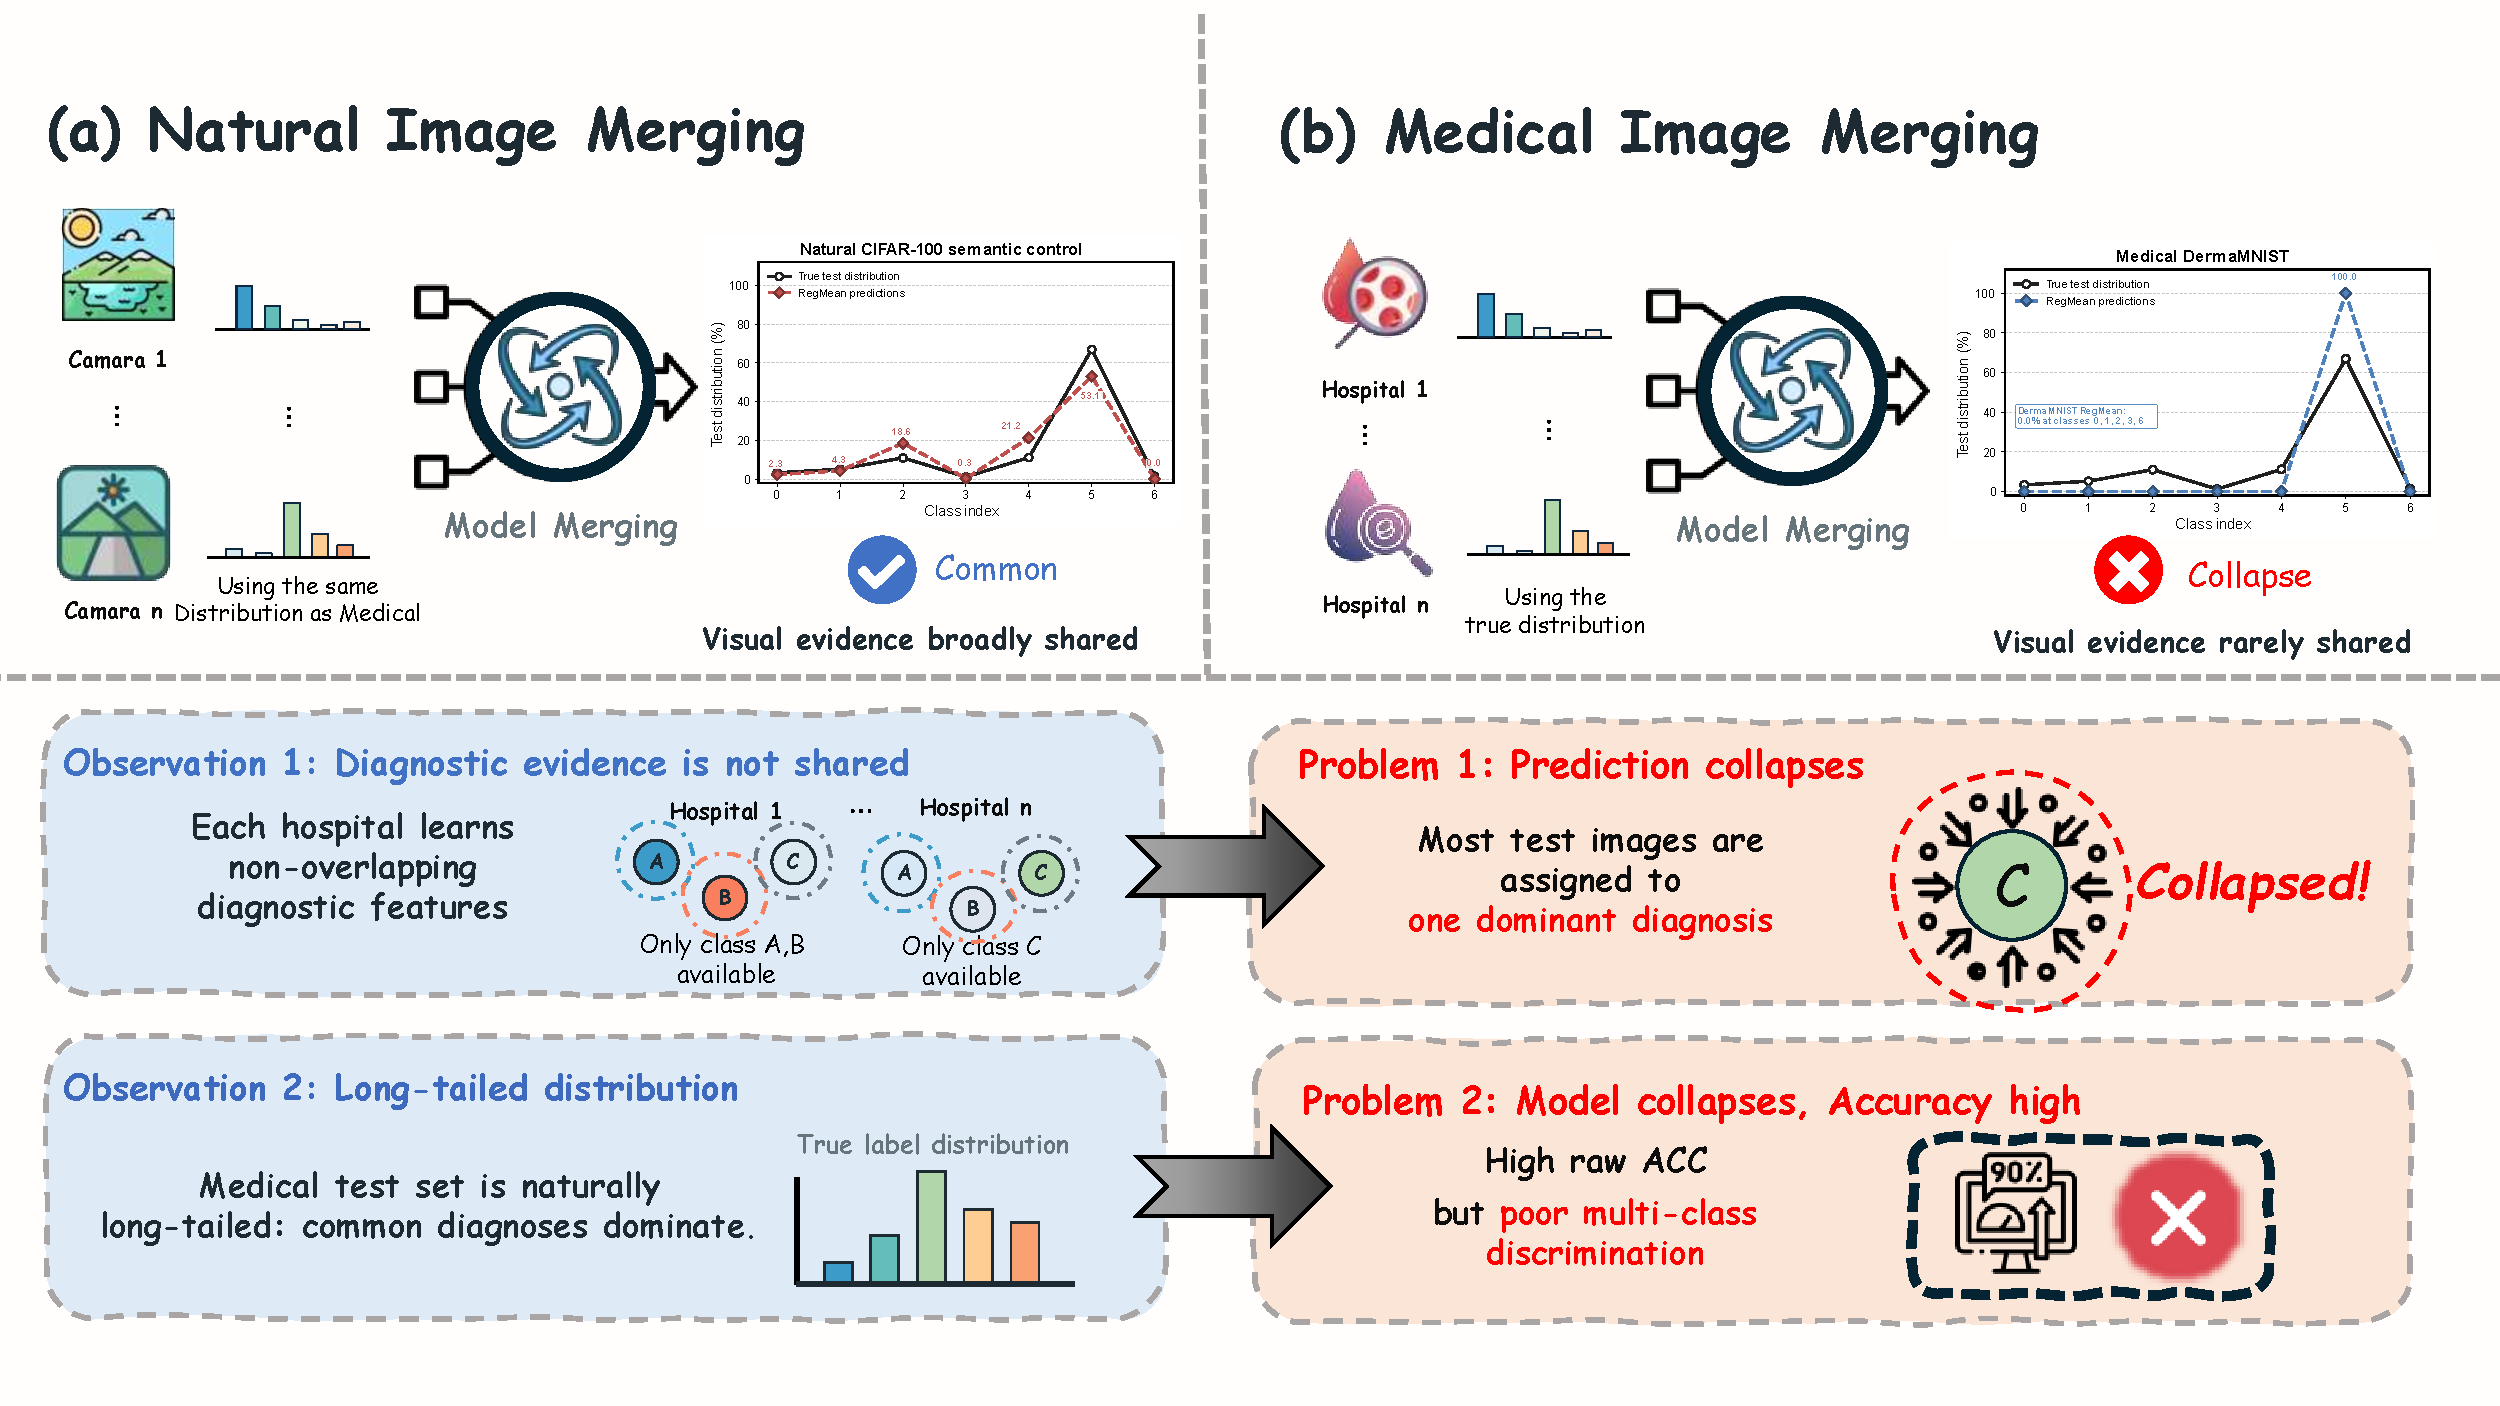
\includegraphics[width=0.96\linewidth]{figures/intro.pdf}
%     \caption{\textbf{Motivation.} Unlike natural-image clients whose generic visual evidence overlaps broadly, medical clients learn client-specific diagnostic evidence that does not transfer across hospitals, so parameter-level merging has little shared structure to align and collapses the global model onto a few dominant classes. This reflects two observations: diagnostic evidence is not shared across isolated clients, and medical prevalence is long-tailed---under which a collapsed model can still report deceptively high accuracy.}
 
%     \label{fig:intro-collapse}
% \end{figure}

% Despite their success on natural images and general visual tasks~\cite{izmailov2018averaging,pmlr-v162-wortsman22a,ilharco2023editingmodelstaskarithmetic,entezari2022role,}, transferring these paradigms to medical data remains challenging. A key reason is that general-purpose model merging implicitly assumes that different client checkpoints contain relatively complete and comparable \textbf{global discriminative structures}; local models are expected to align through parameter space, task-vector space, update signs, or curvature statistics~\cite{yadav2023tiesmergingresolvinginterferencemerging,yu2024languagemodelssupermario,wu_parameter_2025,jin2025datalessknowledgefusionmerging}. This assumption does not hold in medical scenarios. Medical centers differ not only in device domains but also in diagnostic-class availability: some centers may mainly cover common diseases or specific examination types, while having few rare-disease samples~\cite{9557808,10.1371/journal.pmed.1002683,li2021fedbn}. The resulting local models are not complete replicas of the global task, but \textbf{partial diagnostic experts} supported by locally observed diseases.

% As illustrated in Fig.~\ref{fig:intro-collapse}, we summarize these challenges as two diagnostic-structure abnormalities in medical model merging:
% \begin{itemize}
%     \item \textbf{Diagnostic evidence is not shared across medical clients.} Unlike natural images, where generic visual features overlap broadly and give parameter merging a common structure to align, each hospital learns client-specific diagnostic evidence that does not transfer to unobserved classes; local models therefore carry little shared discriminative structure for merging to reconcile~\cite{9557808,li2021fedbn}.
%     \item \textbf{Long-tailed Medical Image Prevalence.} Medical image datasets naturally follow a long-tailed distribution: a few common diagnostic classes dominate the  samples, while rare classes are underrepresented~\cite{BUDA2018249,5597285}. Under this imbalanced class prior, a merged model collapsed to the majority class can still obtain high Accuracy despite lacking complete multi-class discrimination.
% \end{itemize}

% \begin{figure}[!t]
%     \centering
%     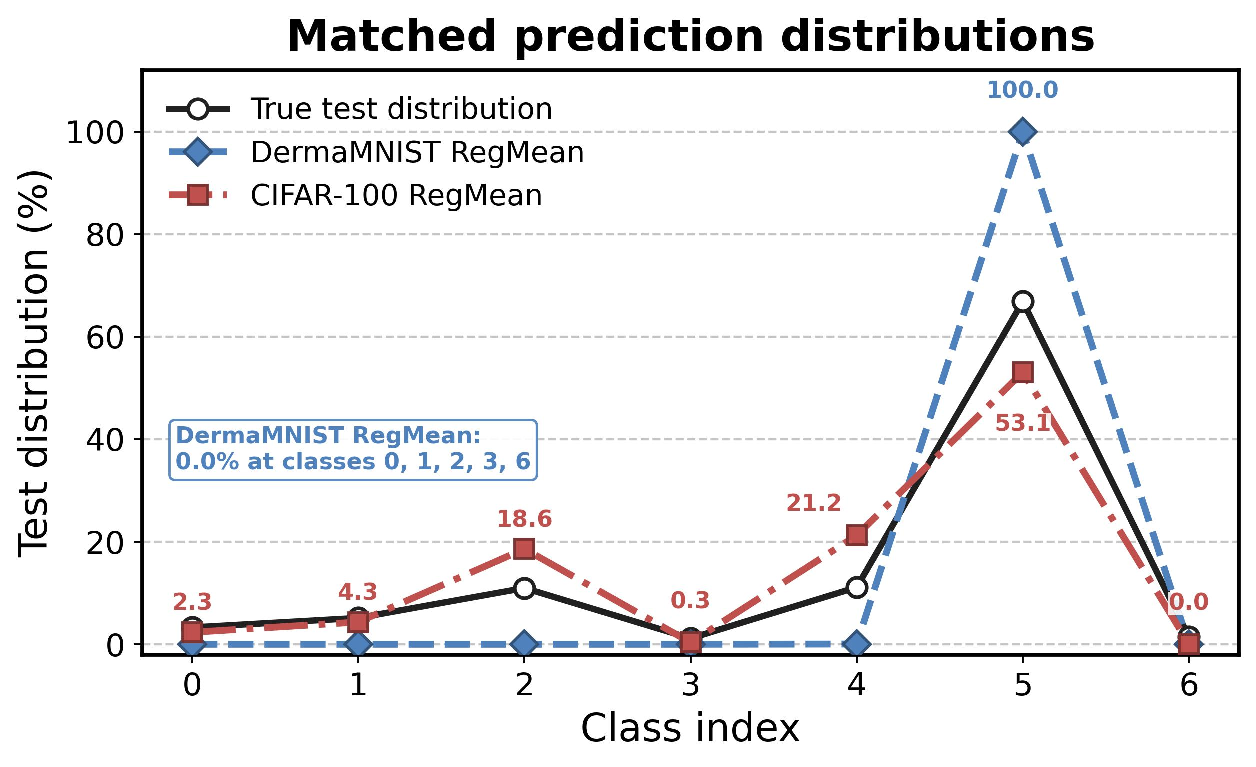
\includegraphics[width=0.96\linewidth]{figures/compare_nl_me.pdf}
%     \caption{\textbf{Collapse is medical-specific, not merging-specific.} Both domains share the \emph{same} class-imbalanced partition template---matched per-class sample counts and matched per-client class assignments---so the only variable is whether the images are natural or medical. Under this controlled setup, the same merging method (RegMean) tracks the true test distribution on natural images (CIFAR-100) but collapses onto a single dominant class on medical images (DermaMNIST: $100\%$ mass on class~5, $0\%$ on classes~0--3 and 6). The pathology is therefore driven by the medical diagnostic structure rather than by the merging operator itself.}
%     \label{fig:collapse-compare}
% \end{figure}

% Fig.~\ref{fig:collapse-compare} confirms that this collapse stems from the medical diagnostic structure rather than from the merging operator itself: with the image domain as the only difference, the same merging method still recovers the multi-class distribution on natural images, yet degenerates onto a single dominant class on medical images.

% To address these issues, we propose \textbf{LAMP-Merge, a long-tail-aware medical prototype-merging method for single-shot asynchronous medical image model merging}. LAMP-Merge shifts the merge target from global parameter interpolation to \textbf{class-level diagnostic-evidence reconstruction}. The key idea is to use client-uploaded class-level statistics as a synchronization signal for the global diagnostic space, allowing the server to reconstruct a global diagnostic classifier without accessing raw medical images, using a server-side validation set, or conducting multi-round federated communication. Specifically, LAMP-Merge consists of two mechanisms: \textbf{diagnostic prototype reconstruction} aggregates reliable class-level evidence through prototypes in a shared reference feature space, and \textbf{long-tail prevalence calibration} injects a bounded prior bias from client-uploaded class counts, thereby mitigating prediction collapse while preserving clinically meaningful majority-class prevalence.

% \begin{figure*}[!t]
%     \centering
%     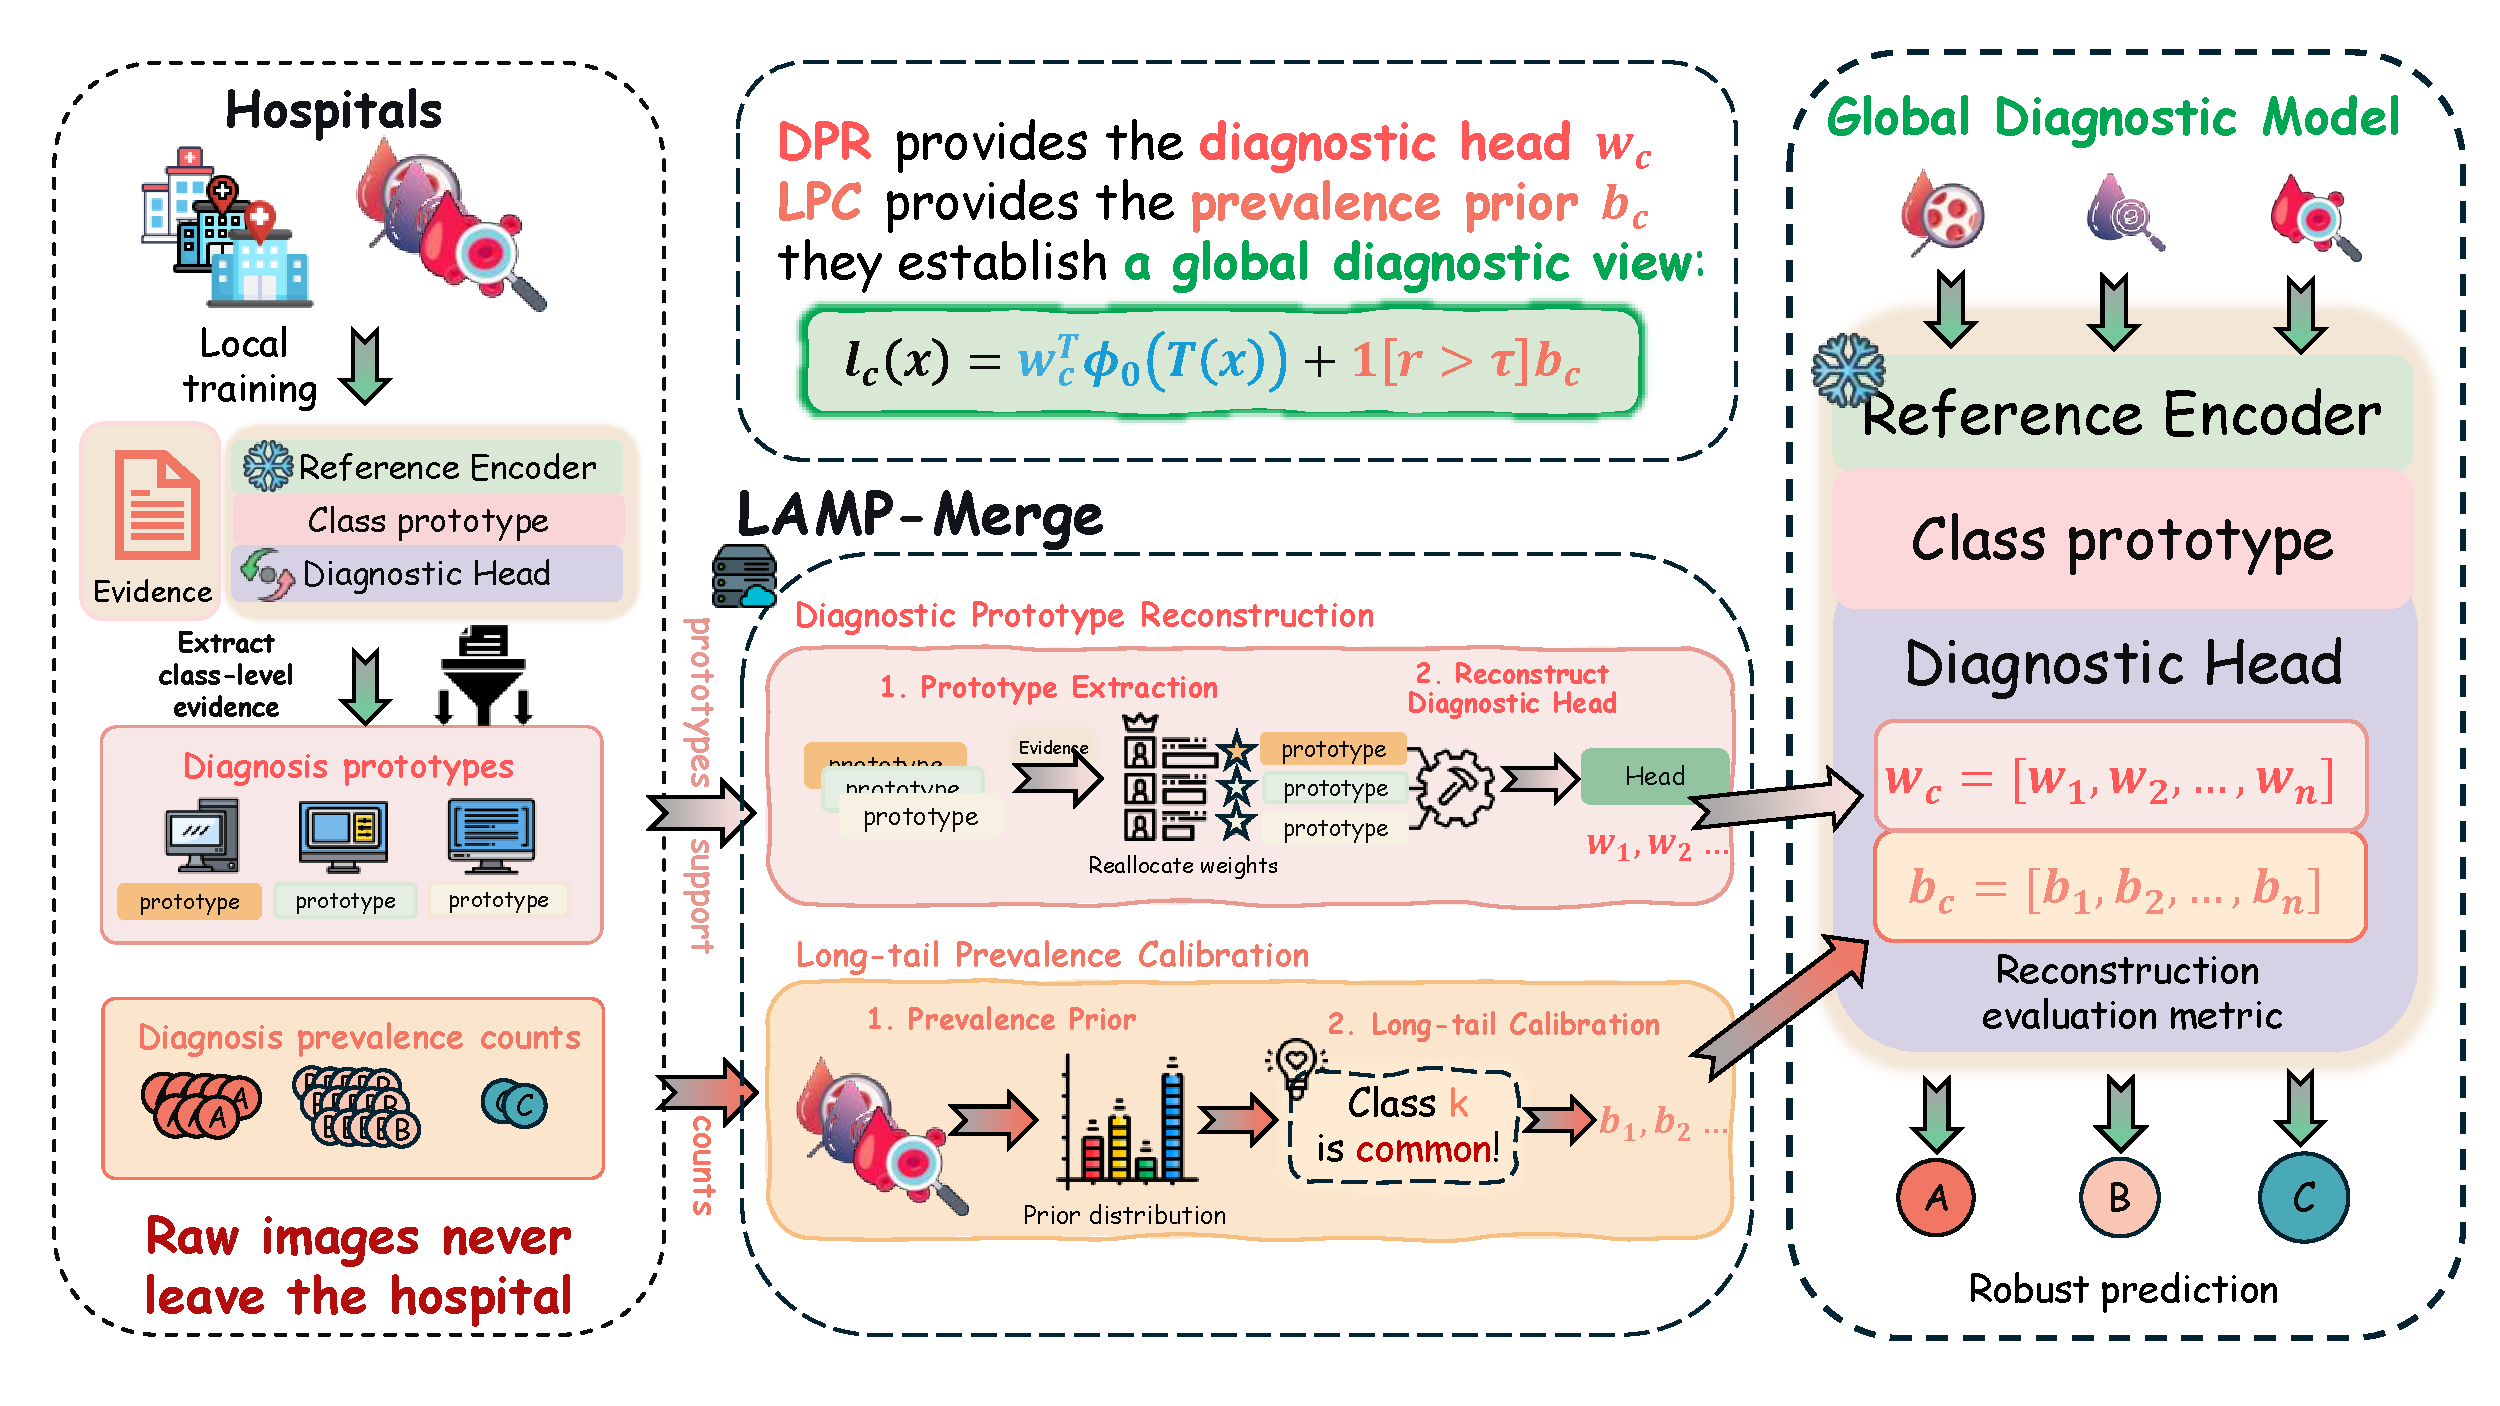
\includegraphics[width=0.92\textwidth,height=0.40\textheight]{figures/method.pdf}
    
%     \caption{\textbf{Overview of LAMP-Merge.} The \textbf{reference encoder} $\phi_0$ is the single frozen encoder that all clients share (the common pretrained backbone before local training); it is called a \textbf{reference} because every hospital expresses its class evidence relative to this one common encoder, so features from different hospitals become directly comparable. Each hospital uploads only class-level statistics---$\phi_0$-space class prototypes with sample support and diagnosis prevalence counts---while raw images stay local. On the server, Diagnostic Prototype Reconstruction (DPR) aggregates the prototypes by support-aware weighting into a diagnostic head $\mathbf{w}_c$, and Long-tail Prevalence Calibration (LPC) adds a gated, bounded log-prior bias $b_c$, giving the scoring rule $\ell_c(x)=\mathbf{w}_c^{\top}\phi_0(T(x))+\mathbf{1}[r>\tau]\,b_c$; the frozen $\phi_0$ is reused as the backbone of the merged model, in a single-shot merge without raw-data sharing or federated rounds.}
 
%     \label{fig_method}
% \end{figure*}

% Our main contributions are summarized as follows:
% \begin{itemize}
%     \item \textbf{Medical Merging Diagnosis.} We revisit model merging under single-shot asynchronous medical collaboration and identify limited local diagnostic coverage and aggregation-induced prediction collapse as two key abnormalities caused by medical class availability and long-tailed prevalence.
%     \item \textbf{LAMP-Merge.} We propose a long-tail-aware medical prototype-merging method that reconstructs a global diagnostic classifier from client-side class prototypes and prevalence statistics without exposing raw images or requiring multi-round federated optimization.
%     \item \textbf{Empirical Validation.} We conduct full-scope experiments on five medical image datasets, four vision-model families, three client-population sizes, and three non-IID skew levels, showing that LAMP-Merge consistently outperforms strong model-merging baselines and improves prediction-collapse diagnostics.
% \end{itemize}

\section{Introduction}

Model merging has emerged as a practical paradigm for integrating independently trained models into a unified model without joint retraining~\cite{ortizjimenez2023tangent,yang2024adamerging}. Unlike federated learning, which relies on repeated collaborative optimization~\cite{pmlr-v54-mcmahan17a,li2020fedprox}, model merging operates after local training and avoids iterative client--server coordination~\cite{stoica2024zipit,wu_parameter_2025}. These properties make model merging a potentially useful interface for multicenter medical collaboration, where raw images cannot easily be centralized and hospitals may not remain online for additional optimization rounds~\cite{kaissis2020secure,bonawitz2019towards,sheller2020federated,rieke2020future,liu2021feddg}. However, whether existing model-merging methods remain effective under medical data heterogeneity is unclear.

\begin{figure}[!t]
    \centering
    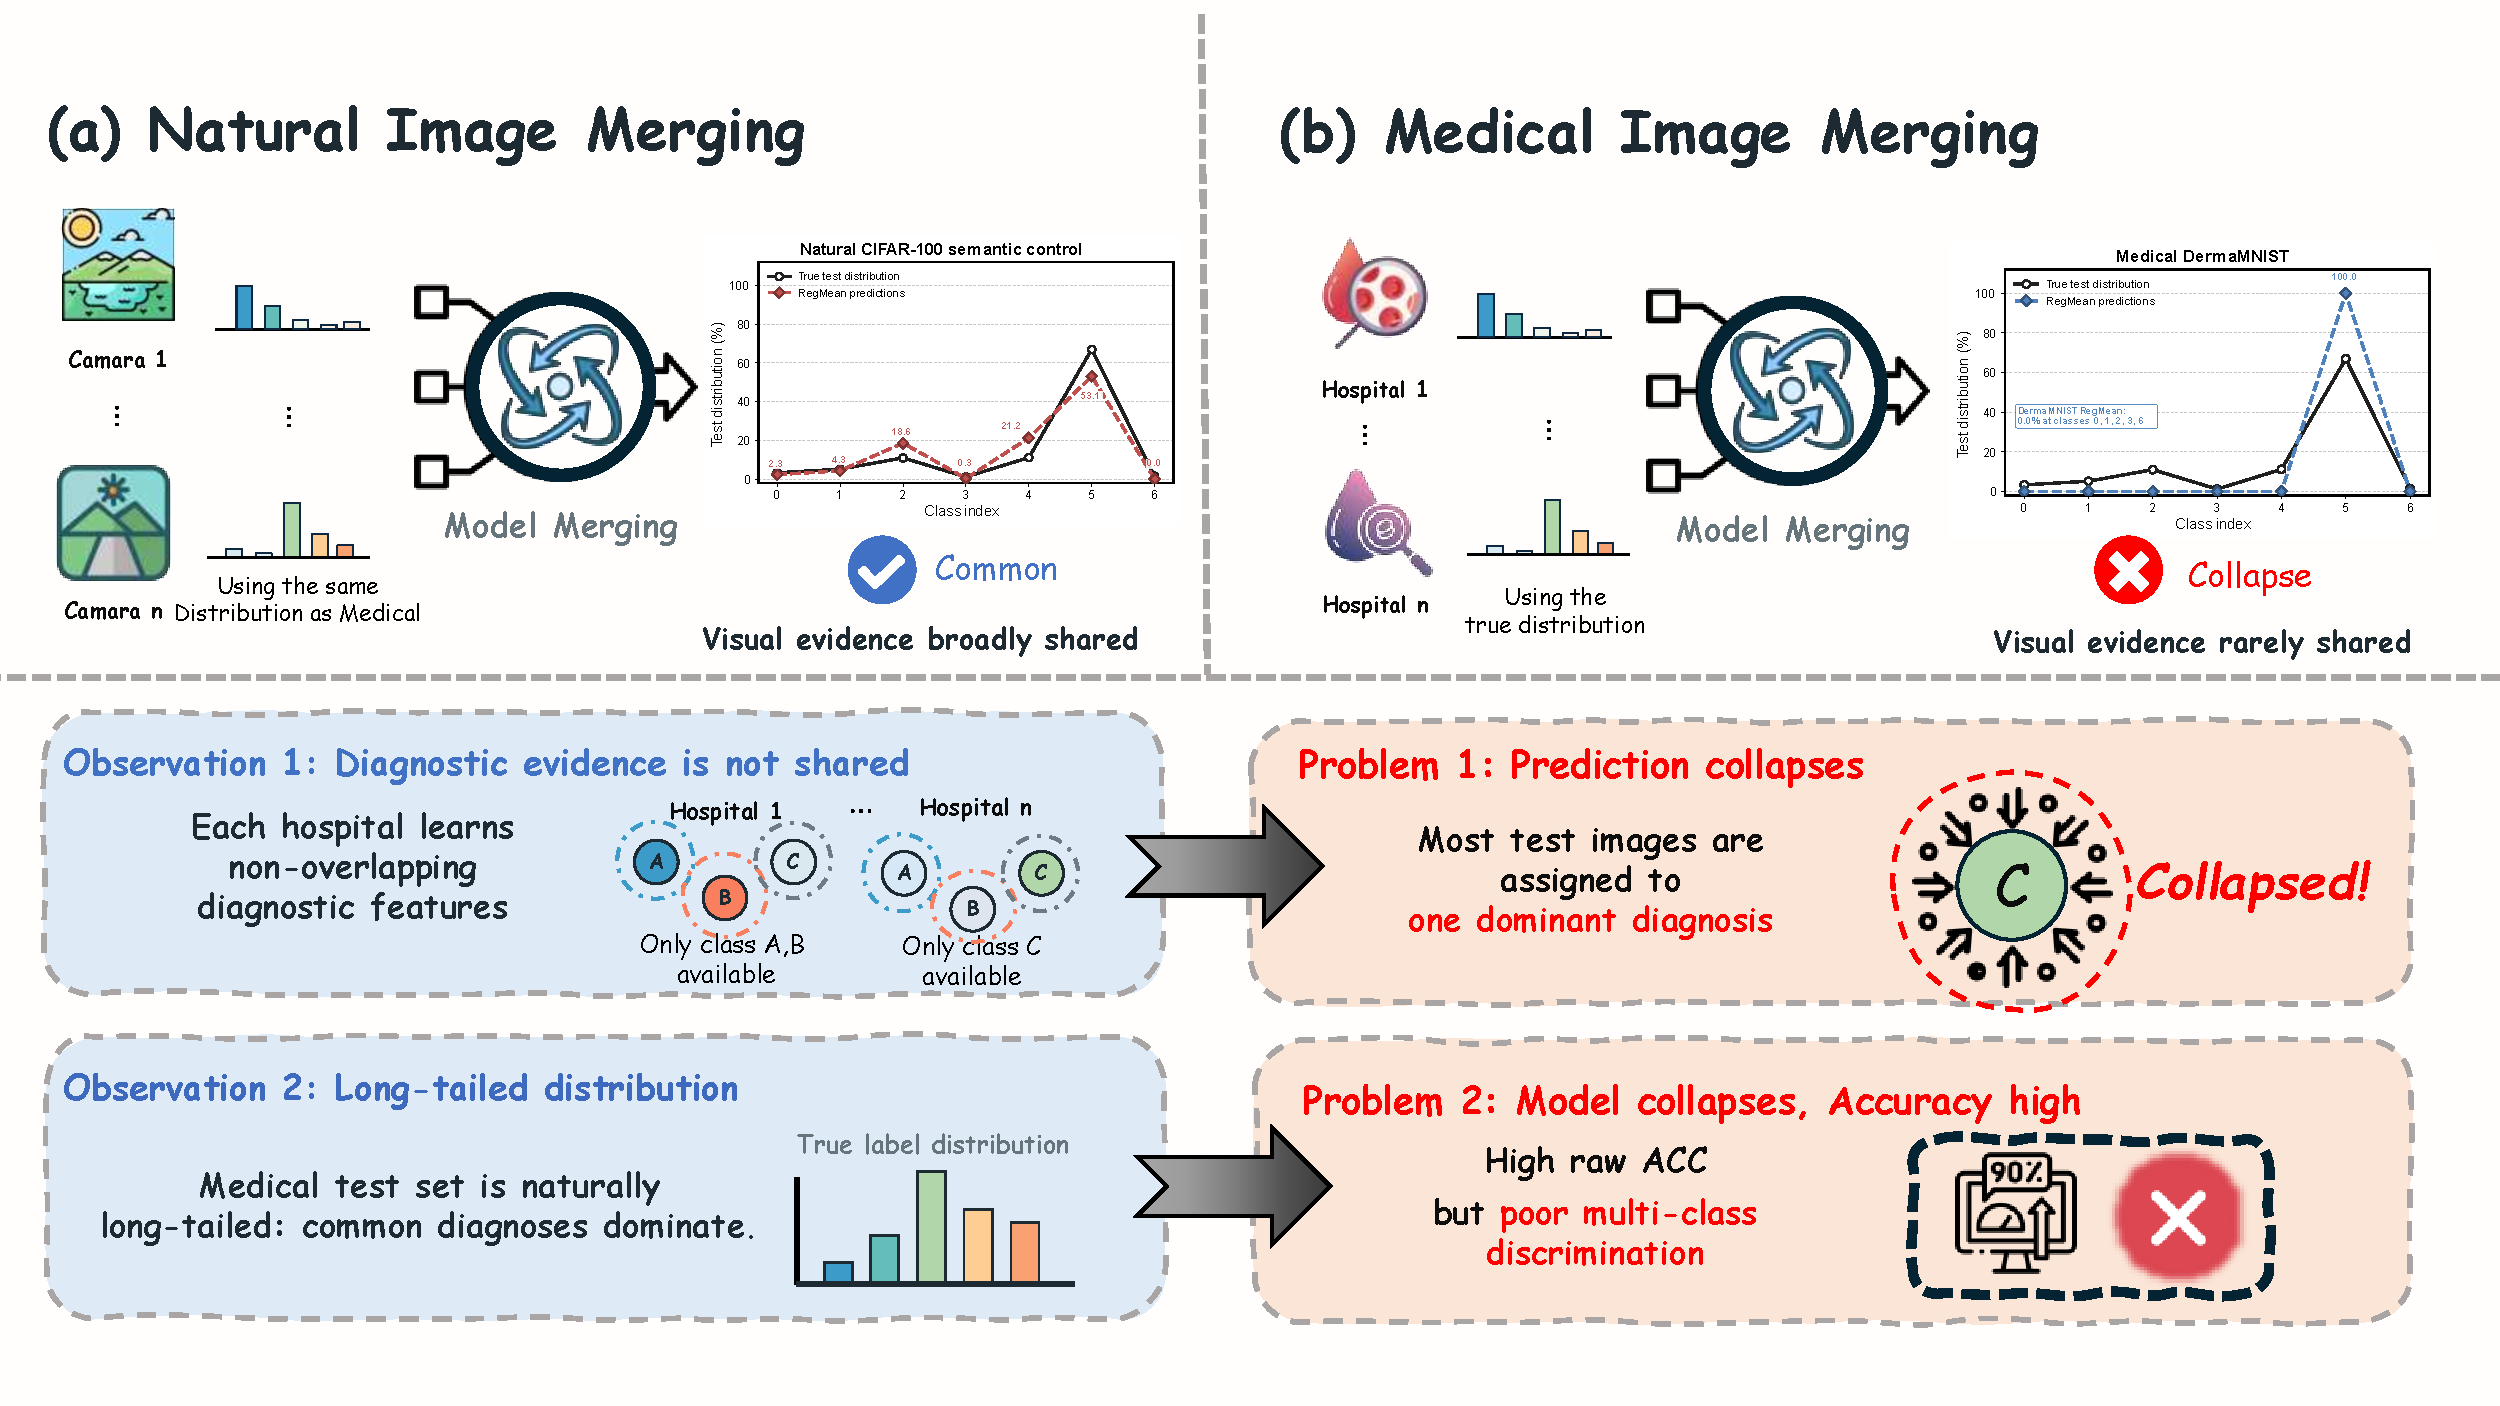
\includegraphics[width=0.96\linewidth]{figures/intro.pdf}
    \caption{\textbf{Motivation.} Left: natural-image models often share broad visual evidence that can be aligned by general-purpose merging. Right: medical centers may cover different diagnosis subsets under long-tailed prevalence, leaving class-agnostic merging unable to distinguish reliable from absent class evidence and potentially concentrating predictions on a few dominant classes.}
 
    \label{fig:intro-collapse}
\end{figure}

Existing model-merging methods combine parameters, task vectors, update signs, or curvature statistics without explicitly tracking class-level support~\cite{izmailov2018averaging,pmlr-v162-wortsman22a,ilharco2023editingmodelstaskarithmetic,entezari2022role,yadav2023tiesmergingresolvinginterferencemerging,yu2024languagemodelssupermario,wu_parameter_2025,jin2025datalessknowledgefusionmerging,matena_merging_2022,huang2024emrmerging,tang2024merging,wang2024localizing}. Applying these class-agnostic operators to medical collaboration is risky: medical data exhibit cross-center domain and prevalence shifts as well as severe class imbalance~\cite{9557808,10.1371/journal.pmed.1002683,li2021fedbn,5597285,zhang2023deeplongtailed}, while a participating hospital in our setting may observe only a subset of diagnostic classes. Model merging can therefore mix reliable class-specific knowledge with models that never observed the corresponding classes.

As illustrated in Fig.~\ref{fig:intro-collapse}, we systematize this mismatch at two coupled levels:
\begin{itemize}
    \item \textbf{Class-discriminative evidence level: aggregation-induced prediction collapse.} Mixing supported and absent class evidence can concentrate predictions on a few dominant diagnoses, while accuracy masks the loss of multiclass discrimination.
    \item \textbf{Prediction-distribution level: long-tailed prevalence preservation.} A dominant prediction may reflect collapse or the observed disease prior; simply flattening the output can therefore erase valid prevalence information.
\end{itemize}

\begin{figure}[!t]
    \centering
    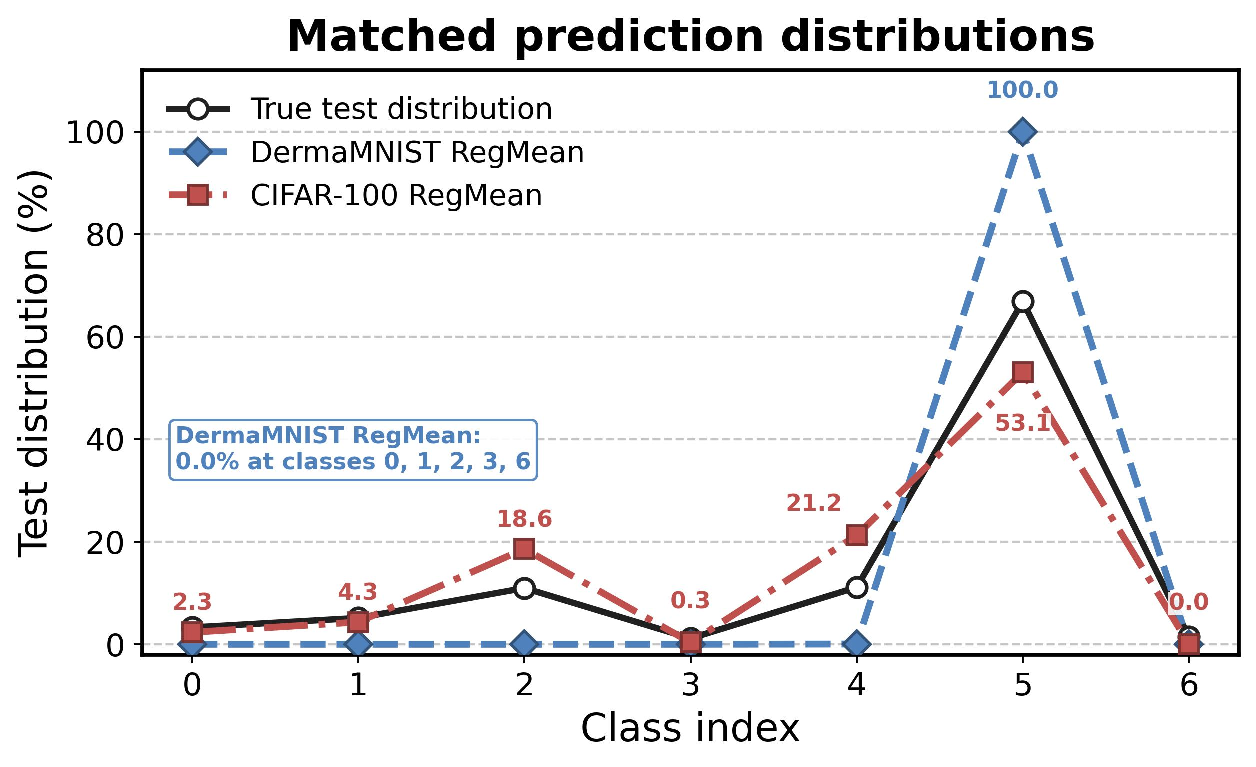
\includegraphics[width=0.85\linewidth]{figures/compare_nl_me.pdf}
    \caption{\textbf{A controlled domain comparison reveals substantially stronger collapse on medical data.} Both domains use matched class-imbalance and client-assignment templates. With the same merging method (RegMean), predictions remain distributed across classes on CIFAR-100 but concentrate entirely on class~5 for DermaMNIST. This contrast suggests that domain-specific data structure can interact adversely with class-agnostic merging.}
    \label{fig:collapse-compare}
\end{figure}

Figure~\ref{fig:collapse-compare} provides controlled evidence of this failure. Under matched class-imbalance and client-assignment templates, RegMean preserves multiclass predictions on CIFAR-100 but assigns every DermaMNIST image to one class. This does not imply that every medical merger must collapse, but it shows that the same merging method can behave differently on medical diagnoses and motivates class-specific reliability. 

Figure~\ref{derma_true} provides data-side evidence for the second observation. DermaMNIST exhibits a clear long-tailed prevalence profile: class~5 alone covers 66.9\% of the test set. Therefore, a medical merger should recover discriminative evidence for minority diagnoses while still preserving valid majority-class prevalence.


\begin{figure}[!t]
    \centering
    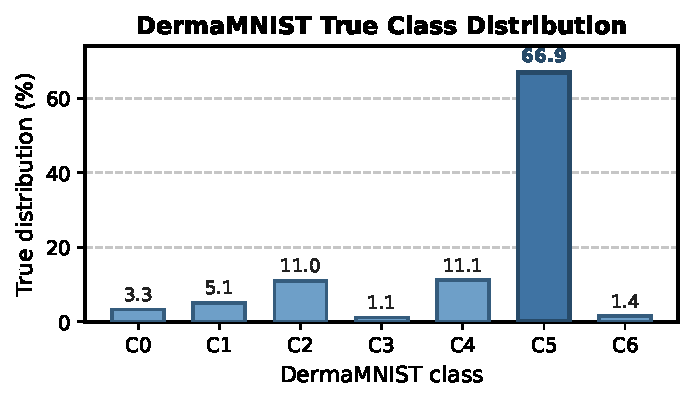
\includegraphics[width=0.85\linewidth]{figures/derma_true_class_distribution.pdf}
    \caption{\textbf{True class distribution reveals a pronounced long-tailed prevalence pattern in medical data}. The figure reports the empirical test distribution of DermaMNIST. The majority class accounts for \textbf{66.9\%} of test images.}
    \label{derma_true}
\end{figure}

To address these problems, we propose \textbf{LAMP-Merge}, a class-aware medical model-merging method that keeps the shared backbone $\phi_0$ frozen and reconstructs the global diagnostic head. \textbf{Diagnostic Prototype Reconstruction (DPR)} merges class prototypes by class-specific support to recover reliable diagnostic directions. \textbf{Long-tail Prevalence Calibration (LPC)} calibrates the reconstructed head using cross-center prevalence statistics without replacing those directions. Together, they construct the global model through one upload of class-level statistics and no further local optimization.

\begin{figure*}[!t]
    \centering
    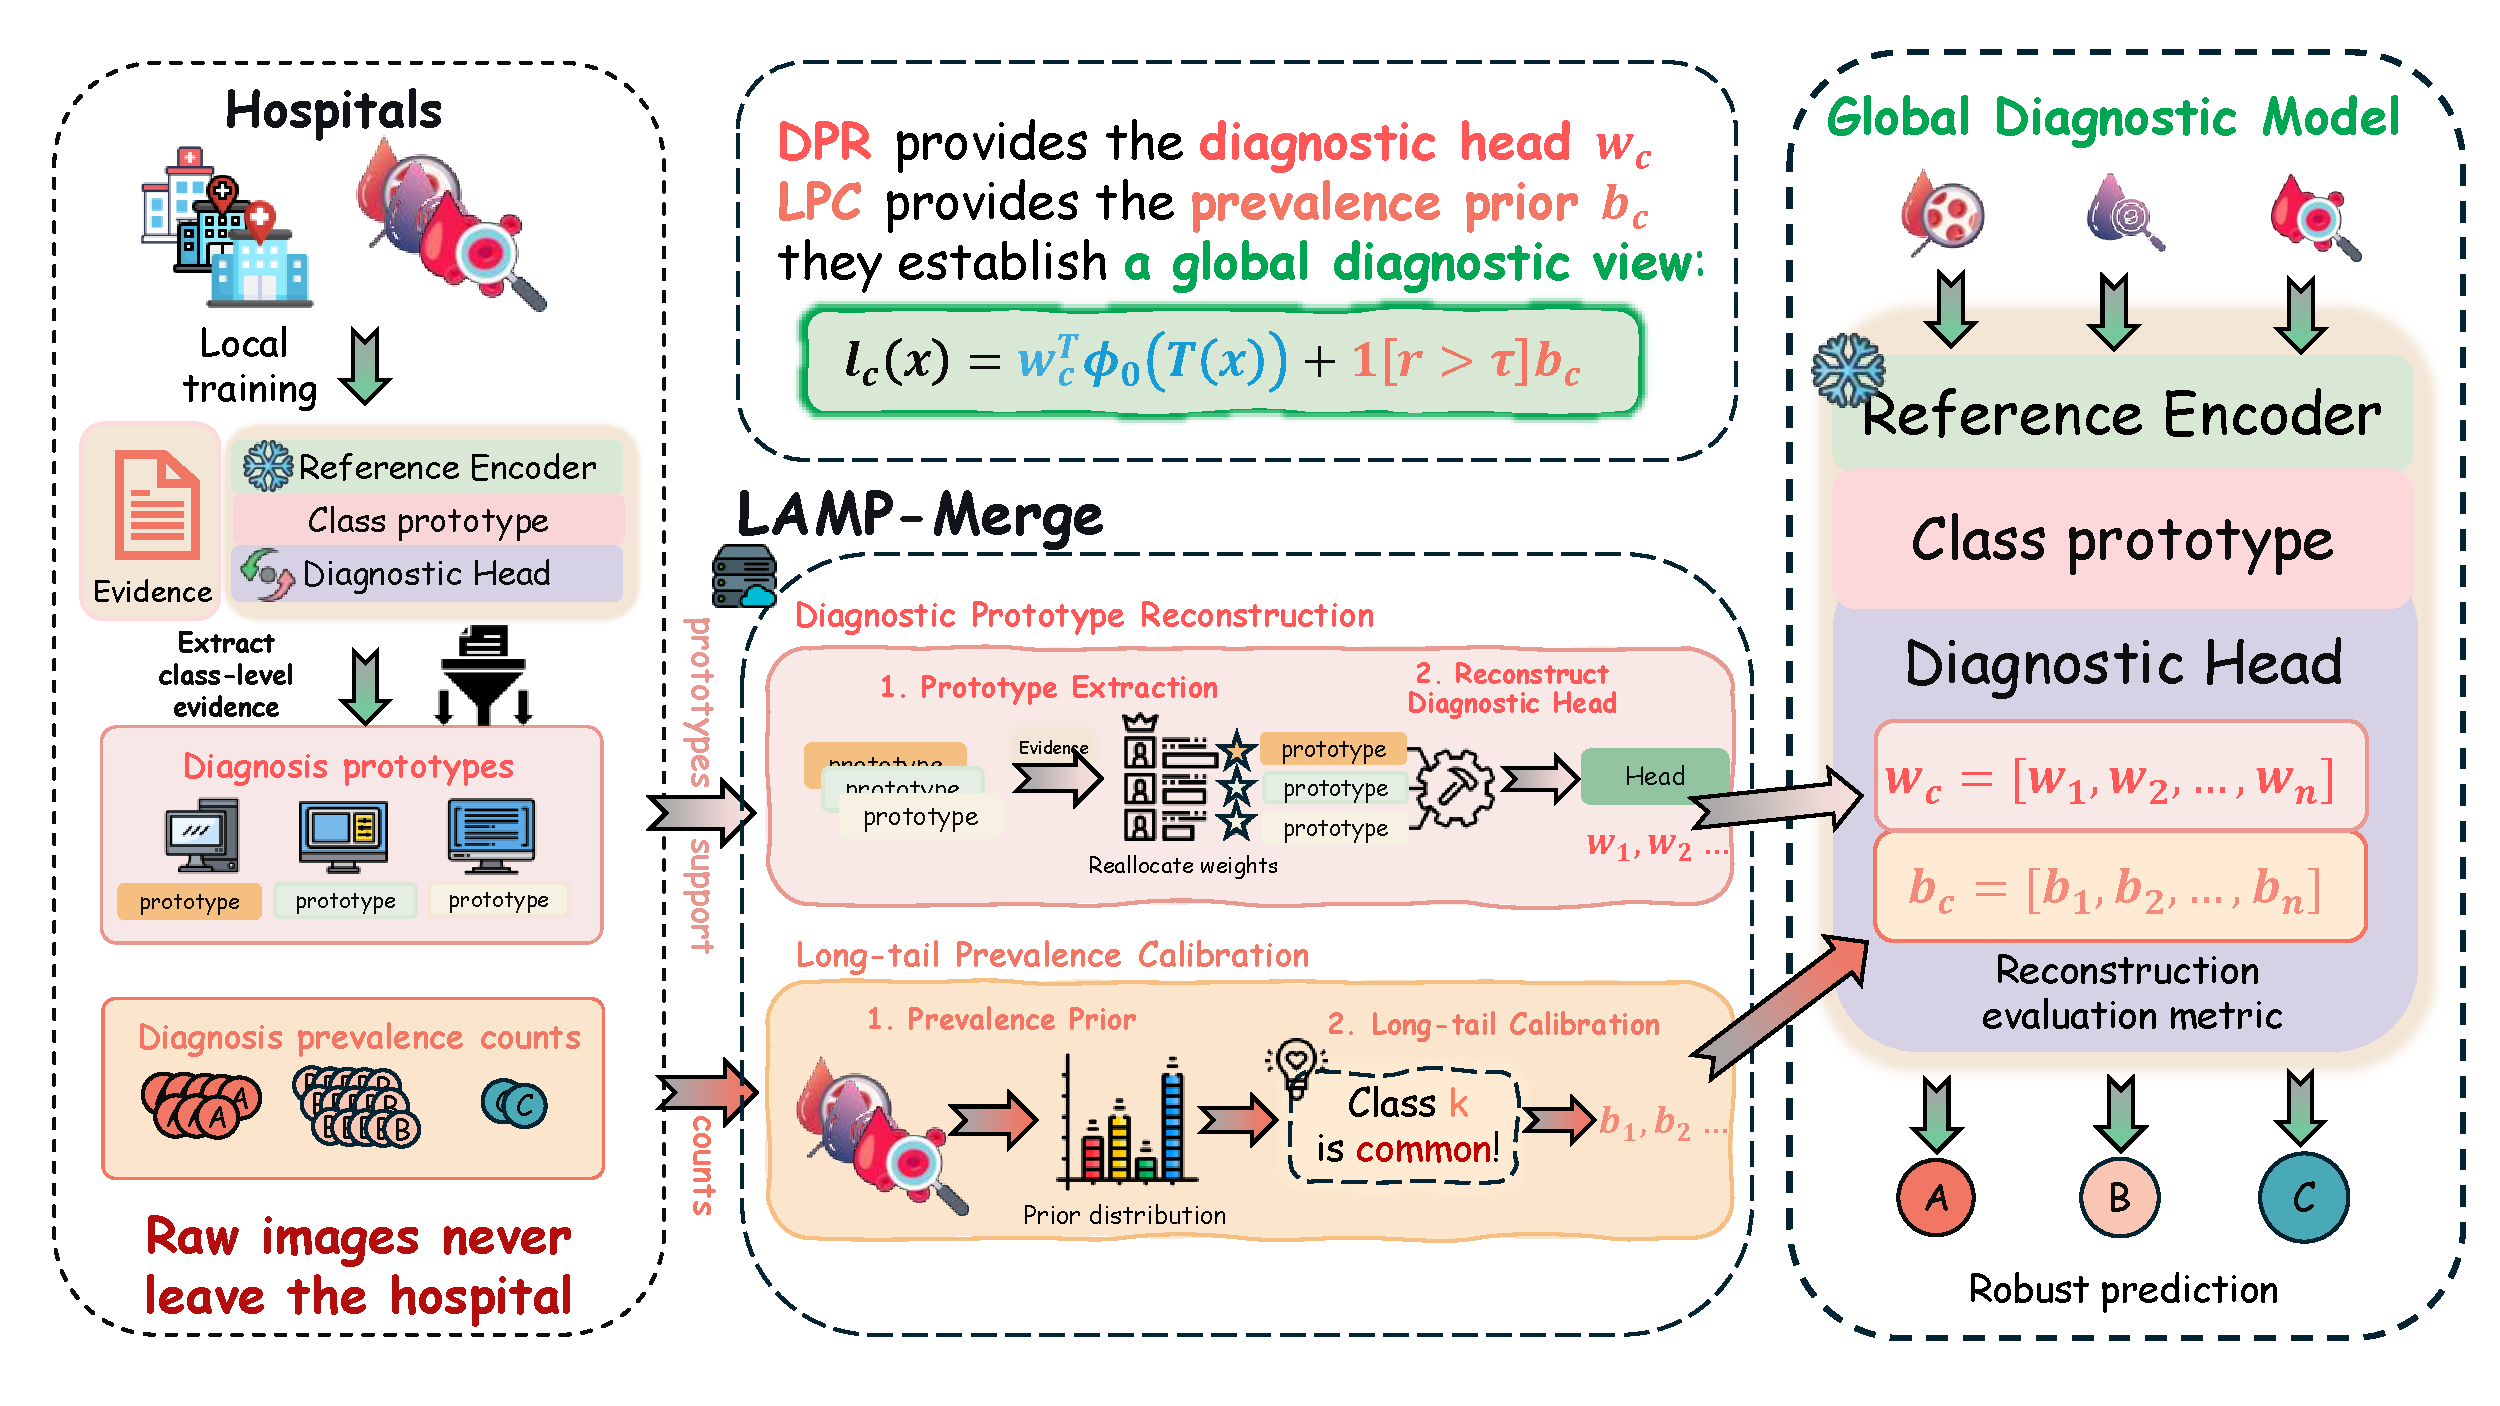
\includegraphics[width=0.80\textwidth,height=0.3\textheight]{figures/method.pdf}
    \caption{\textbf{Overview of LAMP-Merge.} All prototypes and the merged model use the same frozen reference backbone $\phi_0$, and only the diagnostic head is reconstructed. Each hospital uploads class-level statistics---reference-space prototypes with sample support and diagnosis support counts---while raw images stay local. On the server, Diagnostic Prototype Reconstruction (DPR) merges the prototypes by support-aware weighting into the classifier weights $\mathbf{w}_c$, and Long-tail Prevalence Calibration (LPC) adds a gated, scaled, and centered log-prior bias $b_c$. The resulting head is attached to the unchanged $\phi_0$, giving $\ell_c(x)=\mathbf{w}_c^{\top}\phi_0(T(x))+\mathbf{1}[r>\tau]\,b_c$ without raw-data sharing or federated rounds.}
 
    \label{fig_method}
\end{figure*}

We evaluate LAMP-Merge on five medical image datasets spanning microscopy, dermoscopy, CT, and ultrasound, four model families, and diverse client and non-IID settings. It achieves the best dataset-level average accuracy on all five benchmarks among eleven parameter-merging baselines while improving Macro-F1 and prediction-collapse diagnostics. An additional supervised prediction-fusion comparison shows higher overall ACC and Macro-F1 for LAMP-Merge, with task-specific exceptions. Our main contributions are:
\begin{itemize}[leftmargin=*]
    \item[\ding{182}] \textbf{\textit{Problem Identification.}}
    We identify class-evidence dilution and prevalence preservation as two coupled problems in medical model merging and characterize the resulting prediction collapse.
    \item[\ding{183}] \textbf{\textit{Method Design.}}
    We propose LAMP-Merge, combining support-aware prototype reconstruction with prevalence calibration on a shared frozen backbone.
    \item[\ding{184}] \textbf{\textit{Empirical Validation.}}
    Experiments across multiple medical modalities, models, and non-IID settings validate both the method and the identified failure.
\end{itemize}

\section{Related Works}

\subsection{Model Merging}

Model-merging methods integrate independently trained models in parameter, task-vector, or geometric spaces. Weight averaging~\cite{izmailov2018averaging} and Model Soups~\cite{pmlr-v162-wortsman22a} directly interpolate parameters; permutation-aware matching~\cite{entezari2022role} aligns hidden-unit symmetries; ZipIt~\cite{stoica2024zipit} performs feature-level zipping; Task Arithmetic~\cite{ilharco2023editingmodelstaskarithmetic}, its tangent-space refinement~\cite{ortizjimenez2023tangent}, TIES-Merging~\cite{yadav2023tiesmergingresolvinginterferencemerging}, and DARE~\cite{yu2024languagemodelssupermario} manipulate task deltas and sign conflicts; RegMean~\cite{jin2025datalessknowledgefusionmerging}, Model Stock~\cite{jang2025modelstockneedjust}, Breadcrumbs~\cite{davari2024modelbreadcrumbsscalingmultitask}, Iso-C~\cite{marczak2025taskleftbehindisotropic}, FREE-Merging~\cite{zheng2025freemergingfouriertransformefficient}, and RobustMerge~\cite{zeng2025robustmergeparameterefficientmodelmerging} introduce  mean-statistic, subspace, frequency-domain, or robustness assumptions.

However, these methods share a class-agnostic merging interface: their variables are global parameters, task vectors, update signs, or geometric statistics rather than class-level diagnostic evidence. \textbf{They do not encode whether a client has reliable supervision for a specific medical class.} Medical datasets can exhibit substantial cross-center prevalence shifts and class imbalance~\cite{10.1371/journal.pmed.1002683}. Under these conditions and incomplete local class coverage, reliable class directions can be mixed with absent or conflicting directions from other clients, producing the aggregation-induced prediction collapse studied in this paper.

\subsection{Medical Model Merging}

Medical representation-learning and multimodal-fusion studies exploit structures such as irregular clinical time series, physiological sensor graphs, and image--EHR correspondence. mTAN~\cite{shukla2021multitimeattentionnetworksirregularly}, Raindrop~\cite{zhang2022graphguidednetworkirregularlysampled}, and MedFuse~\cite{hayat2023medfusemultimodalfusionclinical} show that medical tasks benefit from modeling clinical sampling mechanisms, modality heterogeneity, and patient-level temporal relations.

Wimmer et al.~\cite{wimmer2022multitaskfusion} provide a non-federated medical model-fusion approach: independently trained task models are combined through prediction-score fusion ($P_{\mathrm{score}}$) or high-level feature fusion ($P_{\mathrm{feat}}$) for mammography classification. This differs from parameter merging because a supervised fusion model learns to combine the retained experts. We include a classification adaptation of their $P_{\mathrm{score}}$-MLP branch as an additional supervised fusion comparator, with its data access and training requirements stated explicitly below.

However, these methods operate on patient-level inputs or multimodal records and require access to those records during training. This data dependence is incompatible with our raw-data-free collaboration constraint~\cite{bonawitz2019towards}. MedMerge~\cite{11382027} is a relevant training-free medical knowledge-transfer framework, but it targets cross-modal adaptation for medical vision-language models rather than model merging for the same classification task. \textbf{Thus, existing medical fusion routes do not match our raw-data-free, single-upload protocol.}
%LAMP-Merge keeps the medical structure uploadable by using only locally computed class prototypes and prevalence counts.

\subsection{Federated Learning}

Federated and decentralized learning perform collaborative training through communication protocols. FedAvg~\cite{pmlr-v54-mcmahan17a} and its variants or medical deployments~\cite{li2020fedprox,karimireddy2020scaffold,li2021fedbn,kaissis2020secure,sheller2020federated,rieke2020future,kairouz2021advances,li2021moon,collins2021fedrep} rely on repeated server-client updates, and Gossip Learning~\cite{hegedhus_gossip_2019} reduce centralization but still require participants to continue training, exchanging models, and optimizing from intermediate states.

Prototype exchange and classifier calibration are closely related to our approach. FedProto~\cite{tan2022fedproto} iteratively exchanges class prototypes and uses global prototypes to regularize local representation learning across heterogeneous clients. Thus, prototype aggregation itself is not new; LAMP-Merge instead uses one upload in a fixed reference space to directly synthesize a diagnostic head, without subsequent local training. CCVR~\cite{luo2021ccvr} is also a post-hoc calibration method: after federated training, it collects class-wise feature means and covariances under the global encoder, samples virtual features, and retrains the classifier. LAMP-Merge uses means and counts without covariance estimation, virtual-feature sampling, or server-side classifier optimization.

CReFF~\cite{shang2022creff} communicates local models and class-wise classifier gradients computed from real features; the server learns federated features by gradient matching and retrains the classifier within an iterative federated procedure. FedLC~\cite{zhang2022fedlc} addresses label skew by label-frequency-dependent logit calibration during local training. In contrast, LPC adds a gated log-prior bias after training, using pooled observed counts. These methods also avoid direct raw-image sharing; our distinction concerns the communication protocol, information supplied, and optimization required, rather than an exclusive privacy property.

Our setting begins after local training has finished. Hospitals may not remain online, receive global checkpoints repeatedly, or run additional optimization rounds. LAMP-Merge therefore targets a single statistics upload and direct head synthesis. This distinguishes it from iterative training approaches, while CCVR remains a relevant post-hoc alternative with different statistics and server optimization requirements.
%LAMP-Merge requires one upload of a local model interface and class-level statistics, enabling the server to construct a unified diagnostic model without a multi-round feedback loop.

\section{Method}
%combine parameters, task vectors, update signs, or curvature statistics
We study post-training medical model merging: \textbf{LAMP-Merge reconstructs the diagnostic head from class-level evidence}, with no raw-data exchange and no federated rounds. The class prototype becomes the unit of merging; this evidence is incomplete when a client has not observed the class and varies in reliability with class-specific support. \textbf{Diagnostic Prototype Reconstruction (DPR)} reconstructs each class direction from the clients that observed it, weighted by class-specific support, while \textbf{Long-tail Prevalence Calibration (LPC)} adds a gated, scaled log-prior to preserve the observed class distribution. Fig.~\ref{fig_method} illustrates the framework.


\subsection{Problem Setting}

Consider $K$ medical clients that share a frozen \textbf{reference encoder} $\phi_0$, the common pretrained backbone every client keeps identical before local training. Client $i$ owns a private labeled dataset $D_i=\{(x,y)\}$ drawn from a class-skewed distribution over $C$ diagnosis classes, with subset $D_{i,c}$ for class $c$. In medical partitions $D_{i,c}$ is empty for many classes: client $i$ carries reliable supervision only for the classes it has observed, and is thus a \textbf{partial diagnostic expert}. After local training, each client makes a \textbf{single upload} of the support count and reference-space prototype for each observed class, never raw images, per-sample features, or a validation set.

\textbf{Shared feature coordinates are a prerequisite for direct prototype aggregation.} All prototypes must be computed with the identical $\phi_0$ and preprocessing $T$, and the merged head must act on that same representation. A common architecture or initialization alone does not ensure this property after independent encoder fine-tuning. Prototypes from independently adapted encoders are outside the scope of the present method: combining them would require an explicit representation-alignment mechanism and constitute a different methodological problem. We assume every evaluated class is observed by at least one participating client.

Keeping raw images local reduces direct exposure of patient-level records, but uploaded prototypes and counts can still disclose sensitive information. Our protocol provides neither differential privacy nor secure aggregation, and we do not claim quantified protection against inference or reconstruction attacks.


\subsection{Diagnostic Prototype Reconstruction}

Generic merging collapses because the diagnostic evidence held by different clients is fragmented and non-comparable in parameter space, so aggregation dilutes it. \textbf{DPR moves the merge into the shared $\phi_0$ space}, where every client's evidence for a class lands in one comparable frame.

With $T(\cdot)$ the evaluation transform, each client summarizes its evidence for class $c$ as the $\phi_0$-space \textbf{class prototype}
\begin{equation}
\mu_{i,c}=\frac{1}{n_{i,c}}\sum_{(x,y)\in D_i}\mathbf{1}[y=c]\,\phi_0(T(x)),
\end{equation}
where $n_{i,c}=|D_{i,c}|$ is the class support and a client with $n_{i,c}=0$ contributes no prototype for that class. Merging class $c$ then reduces to combining the client estimates $\{\mu_{i,c}\}_{i=1}^{K}$ into one global prototype. The key observation is that $\mu_{i,c}$ is a mean over $n_{i,c}$ samples, so a larger support yields a lower-variance estimate; we therefore weight each client by its support,
\begin{equation}
e_{i,c}=(n_{i,c}+1)^{\gamma}\,\mathbf{1}[n_{i,c}>0],\qquad
\alpha_{i,c}=\frac{e_{i,c}}{\sum_{j=1}^{K} e_{j,c}},
\label{eq:support-weight}
\end{equation}
with $\gamma=0.55$ interpolating between uniform ($\gamma=0$) and smoothed support-proportional ($\gamma=1$) averaging. Crucially, $\alpha_{i,c}=0$ whenever $n_{i,c}=0$, so \textbf{absent-class clients can never enter a class reconstruction}. This exclusion prevents models without evidence for class $c$ from diluting its reconstructed direction. The global prototype is then the reliability-weighted average
\begin{equation}
p_c=\sum_{i=1}^{K}\alpha_{i,c}\,\mu_{i,c},\qquad \sum_{i=1}^{K}\alpha_{i,c}=1,
\label{eq:dpr-fuse}
\end{equation}
summing one homogeneous quantity per client like weight averaging, yet reconstructing each class independently. These prototypes finally induce a normalized-weight head
\begin{equation}
w_c=s\,\frac{p_c}{\|p_c\|_2},
\end{equation}
with $s=18.75$. The resulting classifier is \textbf{synthesized from class evidence, not averaged from local classifier weights}.

\textbf{Motivation for support tempering.} In an idealized model with independent class-conditional samples, common mean, and covariance $\Sigma_c$, the sample mean has covariance $\Sigma_c/n_{i,c}$. For nonnegative weights summing to one, the trace variance of their aggregate is $\operatorname{tr}(\Sigma_c)\sum_i\alpha_{i,c}^2/n_{i,c}$, minimized by $\alpha_{i,c}\propto n_{i,c}$ over observing clients. Equation~\ref{eq:support-weight} is a regularized relaxation of this variance-based rule, not its exact minimizer: adding one smooths small supports, while $0<\gamma<1$ compresses the ratio of two clients' weights to $((n_{i,c}+1)/(n_{j,c}+1))^\gamma$. This limits dominance by a large client when the idealized assumptions are imperfect. More precisely, on the simplex of observing clients, the rule maximizes $\sum_i\alpha_i\log(n_{i,c}+1)+H(\alpha)/\gamma$, where $H(\alpha)=-\sum_i\alpha_i\log\alpha_i$. The entropy term trades support preference against concentration, and the mask still excludes absent classes. This motivates the weighting family, but does not establish $\gamma=0.55$ as theoretically optimal; its empirical sensitivity is reported below.

\subsection{Long-tail Prevalence Calibration}

Because the observed class distribution can be long-tailed, collapse correction should not force uniform predictions. DPR alone treats every reconstructed direction symmetrically and encodes no class prior; \textbf{LPC restores this information as a scaled prior on top of the reconstructed head}, distinguishing collapse correction from ordinary class balancing~\cite{cao2019ldam,cui2019classbalanced,kang2020decoupling,ren2020balanced}.

The prior is estimated only from the supported counts uploaded $n_{i,c}$, giving the global class distribution $\pi_c=\big(\sum_{i=1}^{K}n_{i,c}\big)/\big(\sum_{k=1}^{C}\sum_{i=1}^{K}n_{i,k}\big)$. To leave near-balanced tasks untouched, the calibration is \textbf{gated} by the dominant-class imbalance $r=C\max_c\pi_c$ and applied only when $r>\tau$ (default $\tau=2.5$). When active, it adds the centered log-prior bias
\begin{equation}
b_c=\lambda\left(\log\pi_c-\frac{1}{C}\sum_{k=1}^{C}\log\pi_k\right),
\end{equation}
with default strength $\lambda=4.25$. Centering removes the uniform shift, so the bias changes only relative class scores, while the gate prevents unnecessary calibration in near-balanced settings; the reconstructed directions from DPR are thus \textbf{adjusted, never replaced}.

Assembling the two terms gives the score assigned to class $c$ for an input $x$,
\begin{equation}
\ell_c(x)=w_c^{\top}\phi_0(T(x))+\mathbf{1}[r>\tau]\,b_c,
\label{eq:score}
\end{equation}
realized as a single checkpoint. \textbf{Merging is confined entirely to the diagnostic head}: the frozen $\phi_0$ is reused as the shared body, and the head weight and bias are exactly the reconstructed $\{w_c\}$ and calibration $\{b_c\}$. The result $\theta_m=(\phi_0,\{w_c,b_c\})$ is a single global diagnostic model built \textbf{in one pass from class-level prototypes}, with no raw-image access and no federated rounds.
The construction requires only the uploaded prototypes and counts, followed by weighted averaging, normalization, and the gated bias calculation above.



\section{Experiments}

\subsection{Experimental Settings}

\subsubsection{Evaluation datasets.}

We evaluate on four public MedMNIST v2 benchmarks~\cite{yang2023medmnist}---BloodMNIST, DermaMNIST, OrganCMNIST, and OrganSMNIST---and a private eight-class ultrasound subset, ChaoShengMNIST, with anonymized class identifiers. These datasets span blood-cell microscopy, dermoscopy, abdominal CT, and ultrasound, with different class counts and empirical class distributions. Table~\ref{tab:dataset-statistics} summarizes the datasets; Organ-S is included in the five-dataset analyses and the unaveraged results below.



\begin{table}[!t]
\centering
\caption{\textbf{Five medical benchmarks spanning distinct modalities, class counts, and empirical class distributions.} Dataset statistics and a representative sample per benchmark.}
\label{tab:dataset-statistics}
\scriptsize
\renewcommand{\arraystretch}{1.0}
\setlength{\tabcolsep}{2.2pt}
\resizebox{\columnwidth}{!}{%
\begin{tabular}{lrrrrr:c}
\noalign{\hrule height 1.25pt}
\rowcolor[HTML]{F2F2F2}
\textbf{Dataset} & \textbf{Classes} & \textbf{Train} & \textbf{Val} & \textbf{Test} & \textbf{Total} & \textbf{Sample} \\
\hline \hline
Blood & 8 & 11,959 & 1,712 & 3,421 & 17,092 & \makebox[1.05cm][c]{\raisebox{-0.16cm}{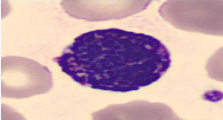
\includegraphics[width=0.95cm,height=0.40cm,keepaspectratio]{figures/sample_blood.pdf}}} \\
\rowcolor{gray!10}
Derma & 7 & 7,007 & 1,003 & 2,005 & 10,015 & \makebox[1.05cm][c]{\raisebox{-0.16cm}{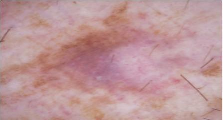
\includegraphics[width=0.95cm,height=0.40cm,keepaspectratio]{figures/sample_derma.pdf}}} \\
Organ-C & 11 & 12,975 & 2,392 & 8,216 & 23,583 & \makebox[1.05cm][c]{\raisebox{-0.16cm}{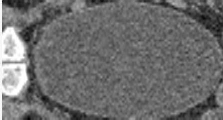
\includegraphics[width=0.95cm,height=0.40cm,keepaspectratio]{figures/sample_organ_c.pdf}}} \\
\rowcolor{gray!10}
Organ-S & 11 & 13,932 & 2,452 & 8,827 & 25,211 & \makebox[1.05cm][c]{\raisebox{-0.16cm}{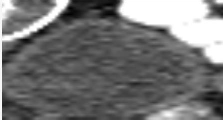
\includegraphics[width=0.95cm,height=0.40cm,keepaspectratio]{figures/sample_organ_s.pdf}}} \\
ChaoShengMNIST & 8 & 3,869 & 549 & 1,113 & 5,531 & \makebox[1.05cm][c]{\raisebox{-0.16cm}{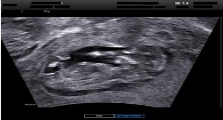
\includegraphics[width=0.95cm,height=0.40cm,keepaspectratio]{figures/sample_ultrasound.pdf}}} \\
\noalign{\hrule height 1.25pt}
\end{tabular}
}
\end{table}

\subsubsection{Comparison baselines.}

The eleven parameter-merging baselines in Tables~\ref{tab:client-avg-swin-tiny}--\ref{tab:client-avg-vit-tiny} retain their own information interfaces; none consumes LAMP-Merge's class-prototype/support-count payload. Parameter-based methods use supervised local-head parameters, task deltas, or their sign and spectral structure. These learned quantities contain information from local images that LAMP-Merge's head synthesis does not use. RegMean additionally uses activation second moments, computed in our implementation from the benchmark validation split; this statistics loader is not restricted to the reconstructed client partitions. Such second moments are not determined by class means and counts. Conversely, LAMP-Merge receives explicit class summaries unavailable to the baseline operators. The comparison therefore evaluates distinct information acquisition and merging procedures on a common reference backbone, rather than identical information budgets. It does not imply that every baseline accesses raw images at server merge time, nor that LAMP-Merge uses validation activations or locally trained head values.

\begin{table*}[!t]
\centering
\renewcommand{\arraystretch}{1.24}
\caption{Client-average test ACC / Macro-F1 (\%) on \textbf{Swin-Tiny}. Each $K$ entry averages three skew settings, and Avg averages the three client counts. The smaller LAMP-Merge line reports the gain over the strongest baseline in the table (pp).}
\label{tab:client-avg-swin-tiny}
\resizebox{\textwidth}{!}{%
\begin{tabular}{l||ccc:c|ccc:c|ccc:c|ccc:c}
\noalign{\hrule height 1.25pt}
\rowcolor[HTML]{F2F2F2}
 &
\multicolumn{4}{c|}{\textbf{Blood}} &
\multicolumn{4}{c|}{\textbf{Derma}} &
\multicolumn{4}{c|}{\textbf{Organ-C}} &
\multicolumn{4}{c}{\textbf{ChaoShengMNIST}} \\
\rowcolor[HTML]{F2F2F2}
\multirow{-2}{*}{\textbf{Method}}
& \textbf{$K=3$} & \textbf{$K=5$} & \textbf{$K=7$} & \textbf{Avg}
& \textbf{$K=3$} & \textbf{$K=5$} & \textbf{$K=7$} & \textbf{Avg}
& \textbf{$K=3$} & \textbf{$K=5$} & \textbf{$K=7$} & \textbf{Avg}
& \textbf{$K=3$} & \textbf{$K=5$} & \textbf{$K=7$} & \textbf{Avg} \\
\hline \hline

Weight Avg.\pub{ICML 2022} & 13.93 / 7.03 & 15.92 / 7.23 & 16.58 / 6.17 & 15.48 / 6.81 & 34.81 / 10.12 & 23.81 / 9.17 & 48.21 / 14.13 & 35.61 / 11.14 & 17.09 / 10.73 & 16.56 / 8.69 & 14.85 / 10.00 & 16.17 / 9.81 & 16.08 / 6.72 & 14.79 / 7.37 & 18.27 / 10.47 & 16.38 / 8.19 \\

\rowcolor{gray!10}
TIES\pub{NeurIPS 2023} & 9.90 / 6.08 & 14.99 / 8.19 & 16.48 / 7.96 & 13.79 / 7.41 & 33.67 / 11.88 & 12.25 / 5.82 & 55.96 / 13.73 & 33.96 / 10.48 & 13.31 / 8.54 & 12.91 / 9.63 & 12.35 / 8.81 & 12.86 / 8.99 & 15.42 / 10.02 & 12.67 / 7.48 & 14.73 / 7.77 & 14.28 / 8.42 \\

DARE-Linear\pub{ICML 2024} & 12.43 / 4.95 & 9.06 / 4.44 & 14.65 / 6.77 & 12.05 / 5.39 & 24.24 / 8.29 & 10.19 / 5.33 & 10.87 / 5.76 & 15.10 / 6.46 & 15.23 / 9.11 & 15.63 / 8.47 & 13.43 / 9.25 & 14.76 / 8.94 & 15.69 / 7.94 & 16.50 / 9.48 & 16.38 / 8.79 & 16.19 / 8.74 \\

\rowcolor{gray!10}
DARE-TIES\pub{ICML 2024} & 11.74 / 3.65 & 7.70 / 4.26 & 12.30 / 4.94 & 10.58 / 4.28 & 26.97 / 10.46 & 10.31 / 4.51 & 44.11 / 13.00 & 27.13 / 9.33 & 12.64 / 7.08 & 11.31 / 7.40 & 11.46 / 8.47 & 11.80 / 7.65 & 14.38 / 9.56 & 15.42 / 9.23 & 14.14 / 9.09 & 14.65 / 9.29 \\

RegMean\pub{ICLR 2023} & 17.36 / 8.43 & 17.68 / 6.95 & 16.17 / 4.92 & 17.07 / 6.76 & 14.00 / 5.68 & 9.89 / 5.26 & 30.06 / 9.38 & 17.98 / 6.78 & 19.61 / 10.28 & 13.81 / 6.79 & 16.26 / 12.08 & 16.56 / 9.72 & 17.25 / 5.64 & 13.99 / 8.16 & 15.51 / 10.27 & 15.58 / 8.02 \\

\rowcolor{gray!10}
Breadcrumbs\pub{ECCV 2024} & 14.41 / 6.42 & 14.64 / 7.39 & 16.34 / 8.34 & 15.13 / 7.38 & 13.53 / 7.23 & 6.05 / 3.61 & 10.41 / 5.67 & 10.00 / 5.50 & 14.62 / 9.57 & 12.62 / 8.39 & 10.20 / 7.95 & 12.48 / 8.64 & 11.62 / 7.20 & 11.17 / 7.73 & 11.23 / 7.27 & 11.34 / 7.40 \\


Model Stock\pub{ECCV 2024} & 16.33 / 8.13 & 15.74 / 6.73 & 16.49 / 6.49 & 16.18 / 7.12 & 28.69 / 9.87 & 15.61 / 6.53 & 30.59 / 11.24 & 24.97 / 9.21 & 16.24 / 10.61 & 16.31 / 9.01 & 15.10 / 9.93 & 15.88 / 9.85 & 15.78 / 7.94 & 15.57 / 9.54 & 15.93 / 10.42 & 15.76 / 9.30 \\

\rowcolor{gray!10}
Iso-C\pub{ICML 2025} & 14.75 / 5.78 & 15.05 / 7.07 & 17.14 / 5.74 & 15.65 / 6.19 & 32.45 / 9.64 & 19.58 / 7.88 & 40.50 / 13.69 & 30.85 / 10.40 & 23.01 / 14.32 & 21.56 / 10.88 & 18.32 / 11.55 & 20.96 / 12.25 & 16.26 / 6.21 & 16.74 / 8.84 & 18.48 / 9.74 & 17.16 / 8.27 \\

FREE-Merging\pub{ICCV 2025} & 13.93 / 7.03 & 15.92 / 7.23 & 16.58 / 6.17 & 15.48 / 6.81 & 34.81 / 10.12 & 23.81 / 9.17 & 48.21 / 14.13 & 35.61 / 11.14 & 17.09 / 10.73 & 16.56 / 8.69 & 14.85 / 10.00 & 16.17 / 9.81 & 16.08 / 6.72 & 14.79 / 7.37 & 18.27 / 10.47 & 16.38 / 8.19 \\

\rowcolor{gray!10}
RobustMerge\pub{NeurIPS 2025} & 17.87 / 7.65 & 15.18 / 7.63 & 17.99 / 6.47 & 17.01 / 7.25 & 10.26 / 6.11 & 8.65 / 4.83 & 13.82 / 7.07 & 10.91 / 6.00 & 13.85 / 8.40 & 18.31 / 10.88 & 13.88 / 8.95 & 15.34 / 9.41 & 11.98 / 6.99 & 13.66 / 8.81 & 13.21 / 9.01 & 12.95 / 8.27 \\


FROM\pub{AAAI 2026} & 12.54 / 4.47 & 15.89 / 7.72 & 15.92 / 6.09 & 14.78 / 6.10 & 35.36 / 12.26 & 17.42 / 7.26 & 58.45 / 14.30 & 37.08 / 11.27 & 14.33 / 8.79 & 16.12 / 9.04 & 13.35 / 8.55 & 14.60 / 8.79 & 18.45 / 8.94 & 14.38 / 7.50 & 15.75 / 7.07 & 16.19 / 7.84 \\

\hdashline
Pscore-MLP (adapted)\pub{TMI 2022} & 50.32 / 38.87 & 59.74 / 49.14 & 67.56 / 61.26 & 59.21 / 49.76 & \textbf{66.70} / 12.25 & \textbf{66.77} / 15.78 & \textbf{66.92} / 16.24 & \textbf{66.79} / 14.76 & 52.84 / 47.49 & 60.45 / 55.97 & 67.02 / 62.92 & 60.10 / 55.46 & 27.52 / 13.53 & 31.57 / 19.86 & 36.66 / 26.09 & 31.92 / 19.83 \\

\hline \hline
\rowcolor[HTML]{FFF9C4}
\textbf{LAMP-Merge} & \tworowbestreshl{\textbf{77.54} / \textbf{75.95}}{+27.22 / +37.08} & \tworowbestreshl{\textbf{77.44} / \textbf{75.77}}{+17.70 / +26.63} & \tworowbestreshl{\textbf{77.30} / \textbf{75.67}}{+9.73 / +14.41} & \tworowbestreshl{\textbf{77.43} / \textbf{75.80}}{+18.22 / +26.04} & \tworowbestreshl{63.24 / \textbf{28.09}}{-3.46 / +15.83} & \tworowbestreshl{63.18 / \textbf{28.24}}{-3.59 / +12.46} & \tworowbestreshl{63.09 / \textbf{27.52}}{-3.82 / +11.28} & \tworowbestreshl{63.17 / \textbf{27.95}}{-3.62 / +13.19} & \tworowbestreshl{\textbf{68.49} / \textbf{65.84}}{+15.64 / +18.35} & \tworowbestreshl{\textbf{68.17} / \textbf{65.38}}{+7.72 / +9.41} & \tworowbestreshl{\textbf{68.12} / \textbf{65.28}}{+1.11 / +2.35} & \tworowbestreshl{\textbf{68.26} / \textbf{65.50}}{+8.16 / +10.04} & \tworowbestreshl{\textbf{47.71} / \textbf{45.76}}{+20.19 / +32.24} & \tworowbestreshl{\textbf{48.70} / \textbf{46.86}}{+17.13 / +27.00} & \tworowbestreshl{\textbf{48.40} / \textbf{46.60}}{+11.74 / +20.50} & \tworowbestreshl{\textbf{48.27} / \textbf{46.41}}{+16.35 / +26.58} \\
\noalign{\hrule height 1.25pt}
\end{tabular}%
}
\end{table*}

\begin{table*}[!t]
\centering
\renewcommand{\arraystretch}{1.24}
\caption{Client-average test ACC / Macro-F1 (\%) on \textbf{ConvNeXt}. Each $K$ entry averages three skew settings, and Avg averages the three client counts. The smaller LAMP-Merge line reports the gain over the strongest baseline in the table (pp).}
\label{tab:client-avg-convnext}
\resizebox{\textwidth}{!}{%
\begin{tabular}{l||ccc:c|ccc:c|ccc:c|ccc:c}
\noalign{\hrule height 1.25pt}
\rowcolor[HTML]{F2F2F2}
 &
\multicolumn{4}{c|}{\textbf{Blood}} &
\multicolumn{4}{c|}{\textbf{Derma}} &
\multicolumn{4}{c|}{\textbf{Organ-C}} &
\multicolumn{4}{c}{\textbf{ChaoShengMNIST}} \\
\rowcolor[HTML]{F2F2F2}
\multirow{-2}{*}{\textbf{Method}}
& \textbf{$K=3$} & \textbf{$K=5$} & \textbf{$K=7$} & \textbf{Avg}
& \textbf{$K=3$} & \textbf{$K=5$} & \textbf{$K=7$} & \textbf{Avg}
& \textbf{$K=3$} & \textbf{$K=5$} & \textbf{$K=7$} & \textbf{Avg}
& \textbf{$K=3$} & \textbf{$K=5$} & \textbf{$K=7$} & \textbf{Avg} \\
\hline \hline

Weight Avg.\pub{ICML 2022} & 25.52 / 11.19 & 18.64 / 7.55 & 28.45 / 13.43 & 24.20 / 10.73 & 51.19 / 11.79 & 50.27 / 12.91 & 58.05 / 14.03 & 53.17 / 12.91 & 9.49 / 6.30 & 9.79 / 7.22 & 11.55 / 8.17 & 10.28 / 7.23 & 19.05 / 7.32 & 13.57 / 5.47 & 17.28 / 11.15 & 16.63 / 7.98 \\

\rowcolor{gray!10}
TIES\pub{NeurIPS 2023} & 21.58 / 9.50 & 21.55 / 7.32 & 20.21 / 8.85 & 21.11 / 8.56 & 34.78 / 10.47 & 42.74 / 11.03 & 28.94 / 9.34 & 35.49 / 10.28 & 11.22 / 7.56 & 12.21 / 9.14 & 13.67 / 9.54 & 12.37 / 8.74 & 14.35 / 6.52 & 11.65 / 5.54 & 9.64 / 5.33 & 11.88 / 5.80 \\

DARE-Linear\pub{ICML 2024} & 18.85 / 10.36 & 18.68 / 12.35 & 24.15 / 13.59 & 20.56 / 12.10 & 51.52 / 12.31 & 20.76 / 7.73 & 30.69 / 10.66 & 34.33 / 10.23 & 10.51 / 8.27 & 8.95 / 7.59 & 10.81 / 9.16 & 10.09 / 8.34 & 19.26 / 6.76 & 15.27 / 6.90 & 16.74 / 10.93 & 17.09 / 8.19 \\

\rowcolor{gray!10}
DARE-TIES\pub{ICML 2024} & 19.89 / 7.59 & 16.15 / 8.57 & 17.00 / 8.55 & 17.68 / 8.24 & 46.63 / 13.49 & 19.09 / 7.00 & 37.92 / 12.06 & 34.55 / 10.85 & 13.41 / 9.72 & 12.37 / 9.18 & 15.26 / 10.53 & 13.68 / 9.81 & 16.65 / 6.57 & 13.57 / 7.32 & 11.74 / 7.16 & 13.99 / 7.02 \\

RegMean\pub{ICLR 2023} & 13.54 / 4.40 & 11.60 / 2.89 & 11.16 / 3.87 & 12.10 / 3.72 & 11.01 / 4.93 & 17.59 / 7.40 & 17.52 / 8.38 & 15.37 / 6.90 & 11.34 / 6.42 & 18.95 / 7.64 & 15.69 / 8.91 & 15.33 / 7.66 & 17.25 / 6.42 & 11.38 / 7.25 & 18.39 / 9.58 & 15.67 / 7.75 \\

\rowcolor{gray!10}
Breadcrumbs\pub{ECCV 2024} & 20.57 / 10.75 & 19.48 / 10.11 & 18.31 / 11.41 & 19.45 / 10.76 & 34.18 / 10.43 & 50.39 / 13.07 & 41.61 / 11.44 & 42.06 / 11.65 & 7.81 / 6.38 & 6.67 / 5.13 & 6.99 / 6.26 & 7.16 / 5.92 & 13.48 / 9.27 & 12.19 / 7.38 & 11.83 / 7.86 & 12.50 / 8.17 \\


Model Stock\pub{ECCV 2024} & 24.90 / 11.42 & 17.70 / 7.77 & 28.59 / 14.20 & 23.73 / 11.13 & 51.40 / 12.30 & 53.98 / 13.98 & 56.91 / 13.68 & 54.10 / 13.32 & 8.48 / 5.95 & 7.83 / 5.75 & 9.34 / 6.84 & 8.55 / 6.18 & 17.01 / 7.66 & 13.24 / 7.52 & 15.45 / 11.49 & 15.23 / 8.89 \\

\rowcolor{gray!10}
Iso-C\pub{ICML 2025} & 27.31 / 12.84 & 18.60 / 7.15 & 31.85 / 15.10 & 25.92 / 11.70 & 60.91 / 13.43 & 52.05 / 13.36 & 59.05 / 14.30 & 57.34 / 13.70 & 10.26 / 7.44 & 10.76 / 8.52 & 12.08 / 8.41 & 11.03 / 8.12 & 19.02 / 7.47 & 13.72 / 6.13 & 17.49 / 11.51 & 16.74 / 8.37 \\


FREE-Merging\pub{ICCV 2025} & 25.52 / 11.19 & 18.64 / 7.55 & 28.45 / 13.43 & 24.20 / 10.73 & 51.19 / 11.79 & 50.27 / 12.91 & 58.05 / 14.03 & 53.17 / 12.91 & 9.49 / 6.30 & 9.79 / 7.22 & 11.55 / 8.17 & 10.28 / 7.23 & 19.05 / 7.32 & 13.57 / 5.47 & 17.28 / 11.15 & 16.63 / 7.98 \\

\rowcolor{gray!10}
RobustMerge\pub{NeurIPS 2025} & 18.72 / 9.23 & 13.23 / 5.89 & 15.76 / 9.70 & 15.90 / 8.27 & 39.27 / 11.14 & 41.75 / 11.19 & 45.70 / 13.07 & 42.24 / 11.80 & 7.45 / 5.88 & 6.36 / 4.54 & 6.36 / 5.77 & 6.72 / 5.40 & 14.56 / 8.64 & 11.47 / 6.44 & 11.35 / 7.24 & 12.46 / 7.44 \\


FROM\pub{AAAI 2026} & 22.15 / 9.09 & 21.76 / 8.02 & 27.35 / 12.69 & 23.75 / 9.93 & 47.51 / 11.24 & 30.12 / 9.82 & 53.97 / 13.54 & 43.87 / 11.53 & 10.39 / 6.27 & 9.17 / 6.63 & 12.29 / 8.40 & 10.62 / 7.10 & 17.55 / 6.65 & 13.72 / 5.53 & 15.84 / 9.17 & 15.70 / 7.12 \\

\hdashline
Pscore-MLP (adapted)\pub{TMI 2022} & 56.89 / 44.71 & 63.32 / 53.45 & 77.48 / 73.24 & 65.90 / 57.13 & \textbf{66.77} / 13.60 & \textbf{67.76} / 17.87 & \textbf{68.43} / 20.03 & \textbf{67.65} / 17.17 & 46.46 / 41.73 & 55.36 / 51.78 & 61.79 / 57.90 & 54.53 / 50.47 & 32.11 / 22.90 & 37.71 / 30.82 & 41.60 / 35.59 & 37.14 / 29.77 \\

\hline \hline
\rowcolor[HTML]{FFF9C4}
\textbf{LAMP-Merge} & \tworowbestreshl{\textbf{85.02} / \textbf{83.45}}{+28.13 / +38.74} & \tworowbestreshl{\textbf{85.02} / \textbf{83.43}}{+21.70 / +29.97} & \tworowbestreshl{\textbf{85.10} / \textbf{83.51}}{+7.62 / +10.27} & \tworowbestreshl{\textbf{85.05} / \textbf{83.46}}{+19.15 / +26.33} & \tworowbestreshl{59.68 / \textbf{33.61}}{-7.08 / +20.01} & \tworowbestreshl{58.77 / \textbf{32.90}}{-8.99 / +15.03} & \tworowbestreshl{59.42 / \textbf{33.33}}{-9.01 / +13.30} & \tworowbestreshl{59.29 / \textbf{33.28}}{-8.36 / +16.11} & \tworowbestreshl{\textbf{65.41} / \textbf{63.18}}{+18.95 / +21.46} & \tworowbestreshl{\textbf{65.33} / \textbf{63.14}}{+9.98 / +11.36} & \tworowbestreshl{\textbf{65.51} / \textbf{63.26}}{+3.72 / +5.36} & \tworowbestreshl{\textbf{65.42} / \textbf{63.19}}{+10.88 / +12.72} & \tworowbestreshl{\textbf{43.07} / \textbf{41.04}}{+10.96 / +18.14} & \tworowbestreshl{\textbf{42.80} / \textbf{40.74}}{+5.09 / +9.92} & \tworowbestreshl{\textbf{42.41} / \textbf{40.40}}{+0.81 / +4.81} & \tworowbestreshl{\textbf{42.76} / \textbf{40.73}}{+5.62 / +10.96} \\
\noalign{\hrule height 1.25pt}
\end{tabular}%
}
\end{table*}

\begin{table*}[!t]
\centering
\renewcommand{\arraystretch}{1.24}
\caption{Client-average test ACC / Macro-F1 (\%) on \textbf{ResNet}. Each $K$ entry averages three skew settings, and Avg averages the three client counts. The smaller LAMP-Merge line reports the gain over the strongest baseline in the table (pp).}
\label{tab:client-avg-resnet}
\resizebox{\textwidth}{!}{%
\begin{tabular}{l||ccc:c|ccc:c|ccc:c|ccc:c}
\noalign{\hrule height 1.25pt}
\rowcolor[HTML]{F2F2F2}
 &
\multicolumn{4}{c|}{\textbf{Blood}} &
\multicolumn{4}{c|}{\textbf{Derma}} &
\multicolumn{4}{c|}{\textbf{Organ-C}} &
\multicolumn{4}{c}{\textbf{ChaoShengMNIST}} \\
\rowcolor[HTML]{F2F2F2}
\multirow{-2}{*}{\textbf{Method}}
& \textbf{$K=3$} & \textbf{$K=5$} & \textbf{$K=7$} & \textbf{Avg}
& \textbf{$K=3$} & \textbf{$K=5$} & \textbf{$K=7$} & \textbf{Avg}
& \textbf{$K=3$} & \textbf{$K=5$} & \textbf{$K=7$} & \textbf{Avg}
& \textbf{$K=3$} & \textbf{$K=5$} & \textbf{$K=7$} & \textbf{Avg} \\
\hline \hline

Weight Avg.\pub{ICML 2022} & 17.58 / 4.80 & 22.68 / 7.71 & 22.40 / 11.05 & 20.89 / 7.85 & 65.97 / 11.91 & 46.50 / 9.86 & 58.70 / 12.17 & 57.06 / 11.31 & 14.56 / 6.98 & 15.58 / 7.63 & 15.77 / 6.26 & 15.30 / 6.96 & 18.63 / 6.51 & 13.24 / 5.23 & 15.81 / 3.69 & 15.89 / 5.15 \\

\rowcolor{gray!10}
TIES\pub{NeurIPS 2023} & 16.96 / 4.70 & 14.07 / 4.53 & 13.74 / 4.63 & 14.92 / 4.62 & 55.68 / 11.10 & 48.21 / 8.57 & 65.92 / 11.97 & 56.60 / 10.55 & 14.67 / 5.31 & 10.74 / 6.00 & 15.10 / 6.45 & 13.50 / 5.92 & 20.84 / 9.96 & 16.11 / 6.75 & 15.93 / 6.92 & 17.63 / 7.88 \\

DARE-Linear\pub{ICML 2024} & 17.37 / 4.96 & 21.04 / 8.93 & 16.02 / 7.46 & 18.14 / 7.12 & 63.04 / 12.32 & 43.97 / 10.91 & 61.38 / 12.91 & 56.13 / 12.05 & 20.31 / 10.18 & 19.38 / 9.37 & 16.11 / 6.61 & 18.60 / 8.72 & 16.98 / 6.98 & 12.52 / 4.74 & 16.38 / 4.80 & 15.29 / 5.51 \\

\rowcolor{gray!10}
DARE-TIES\pub{ICML 2024} & 15.91 / 6.96 & 13.47 / 4.71 & 14.41 / 5.53 & 14.60 / 5.74 & 49.29 / 9.54 & 45.42 / 10.13 & 66.70 / 11.70 & 53.80 / 10.46 & 15.62 / 5.92 & 9.05 / 3.74 & 14.45 / 6.59 & 13.04 / 5.42 & 15.27 / 7.77 & 13.69 / 5.89 & 15.54 / 5.64 & 14.83 / 6.43 \\

RegMean\pub{ICLR 2023} & 18.61 / 6.09 & 14.26 / 6.25 & 18.12 / 8.10 & 17.00 / 6.81 & 48.10 / 10.51 & 17.39 / 9.01 & 23.56 / 9.84 & 29.68 / 9.79 & 17.94 / 9.51 & 16.62 / 9.64 & 15.42 / 9.56 & 16.66 / 9.57 & 16.26 / 7.93 & 14.29 / 9.30 & 12.55 / 6.10 & 14.37 / 7.78 \\

\rowcolor{gray!10}
Breadcrumbs\pub{ECCV 2024} & 18.47 / 7.54 & 13.29 / 6.75 & 18.05 / 8.53 & 16.60 / 7.60 & 39.27 / 10.90 & 21.50 / 7.62 & 28.84 / 10.37 & 29.87 / 9.63 & 9.66 / 4.58 & 8.76 / 5.06 & 11.06 / 4.90 & 9.83 / 4.85 & 12.73 / 7.65 & 11.71 / 6.38 & 12.91 / 5.91 & 12.45 / 6.65 \\


Model Stock\pub{ECCV 2024} & 17.44 / 4.90 & 21.63 / 7.35 & 24.66 / 12.03 & 21.24 / 8.09 & 59.72 / 12.78 & 44.75 / 10.21 & 54.26 / 12.59 & 52.91 / 11.86 & 14.66 / 7.54 & 15.59 / 7.56 & 15.86 / 6.03 & 15.37 / 7.04 & 17.82 / 7.15 & 12.76 / 5.46 & 15.72 / 3.92 & 15.43 / 5.51 \\

\rowcolor{gray!10}
Iso-C\pub{ICML 2025} & 17.30 / 4.41 & 22.68 / 7.68 & 24.30 / 11.92 & 21.43 / 8.00 & 38.99 / 11.09 & 46.12 / 10.83 & 60.71 / 12.59 & 48.61 / 11.50 & 13.46 / 8.63 & 16.88 / 8.30 & 16.50 / 7.44 & 15.61 / 8.12 & 18.84 / 7.13 & 13.93 / 5.17 & 15.30 / 3.83 & 16.02 / 5.38 \\


FREE-Merging\pub{ICCV 2025} & 17.58 / 4.80 & 22.68 / 7.71 & 22.40 / 11.05 & 20.89 / 7.85 & 65.97 / 11.91 & 46.50 / 9.86 & 58.70 / 12.17 & 57.06 / 11.31 & 14.56 / 6.98 & 15.58 / 7.63 & 15.77 / 6.26 & 15.30 / 6.96 & 18.63 / 6.51 & 13.24 / 5.23 & 15.81 / 3.69 & 15.89 / 5.15 \\

\rowcolor{gray!10}
RobustMerge\pub{NeurIPS 2025} & 18.40 / 6.38 & 13.87 / 4.84 & 17.61 / 6.24 & 16.62 / 5.82 & 26.62 / 6.06 & 18.00 / 7.11 & 24.99 / 8.20 & 23.20 / 7.12 & 20.25 / 10.19 & 10.93 / 5.28 & 12.43 / 4.97 & 14.54 / 6.81 & 15.81 / 6.50 & 13.48 / 5.77 & 17.31 / 6.20 & 15.53 / 6.16 \\


FROM\pub{AAAI 2026} & 19.49 / 6.53 & 20.02 / 6.15 & 24.90 / 13.00 & 21.47 / 8.56 & 66.88 / 11.45 & 46.52 / 9.77 & 66.88 / 11.45 & 60.09 / 10.89 & 15.34 / 5.92 & 10.97 / 5.89 & 16.78 / 6.76 & 14.36 / 6.19 & 19.23 / 7.10 & 13.42 / 5.18 & 15.00 / 4.60 & 15.88 / 5.63 \\

\hdashline
Pscore-MLP (adapted)\pub{TMI 2022} & 57.56 / 53.58 & 60.04 / 57.35 & 65.70 / 62.56 & 61.10 / 57.83 & \textbf{67.61} / \textbf{15.55} & \textbf{68.03} / \textbf{17.02} & \textbf{68.65} / \textbf{19.91} & \textbf{68.10} / \textbf{17.50} & 48.60 / 41.09 & 52.60 / 45.22 & 56.28 / 50.17 & 52.49 / 45.49 & 35.46 / 23.79 & 32.82 / 18.81 & 33.84 / 21.19 & 34.04 / 21.26 \\

\hline \hline
\rowcolor[HTML]{FFF9C4}
\textbf{LAMP-Merge} & \tworowbestreshl{\textbf{80.06} / \textbf{78.73}}{+22.51 / +25.15} & \tworowbestreshl{\textbf{79.98} / \textbf{78.66}}{+19.94 / +21.31} & \tworowbestreshl{\textbf{79.97} / \textbf{78.64}}{+14.26 / +16.08} & \tworowbestreshl{\textbf{80.00} / \textbf{78.68}}{+18.90 / +20.85} & \tworowbestreshl{67.55 / 15.03}{-0.07 / -0.53} & \tworowbestreshl{67.63 / 15.16}{-0.40 / -1.87} & \tworowbestreshl{67.63 / 14.94}{-1.01 / -4.97} & \tworowbestreshl{67.60 / 15.04}{-0.49 / -2.45} & \tworowbestreshl{\textbf{60.05} / \textbf{53.11}}{+11.45 / +12.02} & \tworowbestreshl{\textbf{59.94} / \textbf{52.91}}{+7.34 / +7.69} & \tworowbestreshl{\textbf{60.07} / \textbf{53.30}}{+3.80 / +3.13} & \tworowbestreshl{\textbf{60.02} / \textbf{53.11}}{+7.53 / +7.61} & \tworowbestreshl{\textbf{48.07} / \textbf{45.96}}{+12.61 / +22.16} & \tworowbestreshl{\textbf{46.75} / \textbf{44.50}}{+13.93 / +25.69} & \tworowbestreshl{\textbf{47.35} / \textbf{45.05}}{+13.51 / +23.86} & \tworowbestreshl{\textbf{47.39} / \textbf{45.17}}{+13.35 / +23.90} \\
\noalign{\hrule height 1.25pt}
\end{tabular}%
}
\end{table*}

\begin{table*}[!t]
\centering
\renewcommand{\arraystretch}{1.24}
\caption{Client-average test ACC / Macro-F1 (\%) on \textbf{ViT-Tiny}. Each $K$ entry averages three skew settings, and Avg averages the three client counts. The smaller LAMP-Merge line reports the gain over the strongest baseline in the table (pp).}
\label{tab:client-avg-vit-tiny}
\resizebox{\textwidth}{!}{%
\begin{tabular}{l||ccc:c|ccc:c|ccc:c|ccc:c}
\noalign{\hrule height 1.25pt}
\rowcolor[HTML]{F2F2F2}
 &
\multicolumn{4}{c|}{\textbf{Blood}} &
\multicolumn{4}{c|}{\textbf{Derma}} &
\multicolumn{4}{c|}{\textbf{Organ-C}} &
\multicolumn{4}{c}{\textbf{ChaoShengMNIST}} \\
\rowcolor[HTML]{F2F2F2}
\multirow{-2}{*}{\textbf{Method}}
& \textbf{$K=3$} & \textbf{$K=5$} & \textbf{$K=7$} & \textbf{Avg}
& \textbf{$K=3$} & \textbf{$K=5$} & \textbf{$K=7$} & \textbf{Avg}
& \textbf{$K=3$} & \textbf{$K=5$} & \textbf{$K=7$} & \textbf{Avg}
& \textbf{$K=3$} & \textbf{$K=5$} & \textbf{$K=7$} & \textbf{Avg} \\
\hline \hline

Weight Avg.\pub{ICML 2022} & 14.57 / 6.21 & 15.91 / 5.46 & 16.24 / 11.40 & 15.57 / 7.69 & 39.32 / 10.78 & 55.05 / 12.49 & 48.25 / 11.54 & 47.54 / 11.60 & 11.29 / 7.13 & 10.50 / 7.95 & 6.62 / 4.54 & 9.47 / 6.54 & 14.53 / 5.62 & 13.33 / 5.68 & 14.44 / 6.12 & 14.10 / 5.81 \\

\rowcolor{gray!10}
TIES\pub{NeurIPS 2023} & 17.16 / 7.68 & 14.43 / 5.25 & 13.62 / 7.31 & 15.07 / 6.75 & 47.32 / 12.75 & 39.75 / 9.94 & 38.64 / 12.37 & 41.90 / 11.69 & 10.73 / 6.46 & 9.18 / 5.28 & 7.42 / 5.61 & 9.11 / 5.78 & 16.71 / 9.92 & 15.06 / 8.18 & 14.05 / 8.36 & 15.27 / 8.82 \\

DARE-Linear\pub{ICML 2024} & 10.79 / 5.95 & 12.77 / 8.47 & 11.17 / 7.90 & 11.58 / 7.44 & 19.83 / 8.08 & 21.46 / 7.74 & 20.80 / 7.15 & 20.70 / 7.66 & 10.30 / 6.23 & 7.75 / 3.92 & 5.98 / 2.90 & 8.01 / 4.35 & 13.06 / 6.48 & 15.93 / 8.05 & 16.14 / 7.33 & 15.04 / 7.28 \\

\rowcolor{gray!10}
DARE-TIES\pub{ICML 2024} & 13.56 / 10.31 & 11.11 / 5.48 & 20.37 / 9.21 & 15.02 / 8.33 & 12.97 / 7.32 & 35.66 / 12.20 & 48.88 / 15.62 & 32.50 / 11.71 & 9.66 / 5.57 & 7.36 / 5.17 & 5.93 / 3.97 & 7.65 / 4.90 & 14.38 / 9.59 & 13.66 / 8.05 & 13.84 / 10.15 & 13.96 / 9.26 \\

RegMean\pub{ICLR 2023} & 13.56 / 4.54 & 10.42 / 3.13 & 11.88 / 5.55 & 11.95 / 4.41 & 51.65 / 12.19 & 23.92 / 8.29 & 29.98 / 8.96 & 35.18 / 9.81 & 15.90 / 8.61 & 10.46 / 5.90 & 11.47 / 8.72 & 12.61 / 7.74 & 14.29 / 8.10 & 15.48 / 8.07 & 15.42 / 9.69 & 15.06 / 8.62 \\

\rowcolor{gray!10}
Breadcrumbs\pub{ECCV 2024} & 9.08 / 6.40 & 12.05 / 6.19 & 11.80 / 6.32 & 10.98 / 6.30 & 25.15 / 9.25 & 12.42 / 6.54 & 16.72 / 7.33 & 18.10 / 7.71 & 5.94 / 3.26 & 4.86 / 2.57 & 4.16 / 2.90 & 4.98 / 2.91 & 12.70 / 6.03 & 12.91 / 6.90 & 13.36 / 6.46 & 12.99 / 6.46 \\


Model Stock\pub{ECCV 2024} & 12.22 / 6.19 & 14.95 / 7.49 & 10.33 / 6.51 & 12.50 / 6.73 & 34.70 / 10.35 & 48.50 / 12.20 & 42.58 / 11.57 & 41.92 / 11.38 & 9.47 / 6.00 & 7.78 / 5.48 & 6.16 / 3.68 & 7.80 / 5.06 & 12.82 / 5.21 & 13.00 / 5.96 & 13.57 / 4.65 & 13.13 / 5.27 \\

\rowcolor{gray!10}
Iso-C\pub{ICML 2025} & 16.18 / 6.74 & 18.51 / 7.03 & 12.54 / 8.97 & 15.75 / 7.58 & 37.76 / 10.19 & 56.24 / 13.27 & 50.22 / 11.92 & 48.07 / 11.79 & 11.15 / 7.54 & 11.02 / 8.25 & 6.97 / 4.85 & 9.71 / 6.88 & 13.57 / 4.61 & 12.85 / 5.37 & 12.91 / 4.40 & 13.11 / 4.79 \\


FREE-Merging\pub{ICCV 2025} & 14.57 / 6.21 & 15.91 / 5.46 & 16.24 / 11.40 & 15.57 / 7.69 & 39.32 / 10.78 & 55.05 / 12.49 & 48.25 / 11.54 & 47.54 / 11.60 & 11.29 / 7.13 & 10.50 / 7.95 & 6.62 / 4.54 & 9.47 / 6.54 & 14.53 / 5.62 & 13.33 / 5.68 & 14.44 / 6.12 & 14.10 / 5.81 \\

\rowcolor{gray!10}
RobustMerge\pub{NeurIPS 2025} & 11.97 / 6.52 & 14.51 / 6.85 & 9.57 / 4.46 & 12.01 / 5.94 & 29.14 / 9.93 & 30.46 / 9.57 & 52.12 / 12.97 & 37.24 / 10.82 & 7.11 / 3.62 & 6.82 / 3.32 & 6.66 / 3.12 & 6.86 / 3.35 & 14.20 / 7.10 & 14.59 / 7.17 & 14.56 / 8.34 & 14.45 / 7.54 \\


FROM\pub{AAAI 2026} & 20.51 / 9.14 & 15.88 / 4.30 & 19.61 / 10.27 & 18.67 / 7.90 & 54.83 / 13.31 & 54.48 / 11.19 & 59.82 / 13.11 & 56.38 / 12.54 & 11.88 / 7.34 & 10.75 / 7.40 & 7.40 / 4.70 & 10.01 / 6.48 & 15.30 / 8.17 & 12.28 / 5.00 & 13.63 / 5.86 & 13.74 / 6.34 \\

\hdashline
Pscore-MLP (adapted)\pub{TMI 2022} & 64.65 / 60.00 & 71.33 / 67.18 & 82.00 / 79.67 & 72.66 / 68.95 & \textbf{67.20} / 14.85 & \textbf{69.14} / 21.51 & \textbf{70.67} / 28.66 & \textbf{69.01} / 21.67 & 55.44 / 50.87 & \textbf{64.95} / \textbf{61.09} & \textbf{68.98} / \textbf{65.60} & \textbf{63.12} / \textbf{59.19} & 33.27 / 22.12 & 38.04 / 29.26 & 45.73 / 40.68 & 39.01 / 30.69 \\

\hline \hline
\rowcolor[HTML]{FFF9C4}
\textbf{LAMP-Merge} & \tworowbestreshl{\textbf{85.32} / \textbf{83.09}}{+20.67 / +23.09} & \tworowbestreshl{\textbf{85.16} / \textbf{82.94}}{+13.83 / +15.75} & \tworowbestreshl{\textbf{85.16} / \textbf{82.87}}{+3.16 / +3.19} & \tworowbestreshl{\textbf{85.21} / \textbf{82.96}}{+12.55 / +14.01} & \tworowbestreshl{59.45 / \textbf{36.60}}{-7.75 / +21.75} & \tworowbestreshl{59.32 / \textbf{36.50}}{-9.83 / +14.99} & \tworowbestreshl{59.83 / \textbf{36.79}}{-10.84 / +8.13} & \tworowbestreshl{59.53 / \textbf{36.63}}{-9.47 / +14.96} & \tworowbestreshl{\textbf{58.78} / \textbf{57.43}}{+3.34 / +6.56} & \tworowbestreshl{58.40 / 56.94}{-6.55 / -4.15} & \tworowbestreshl{58.29 / 56.80}{-10.68 / -8.80} & \tworowbestreshl{58.49 / 57.06}{-4.63 / -2.13} & \tworowbestreshl{\textbf{46.12} / \textbf{42.32}}{+12.85 / +20.20} & \tworowbestreshl{\textbf{45.97} / \textbf{42.19}}{+7.94 / +12.93} & \tworowbestreshl{\textbf{45.94} / \textbf{42.23}}{+0.21 / +1.55} & \tworowbestreshl{\textbf{46.01} / \textbf{42.25}}{+7.00 / +11.56} \\
\noalign{\hrule height 1.25pt}
\end{tabular}%
}
\end{table*}

We compare LAMP-Merge with eleven model-merging baselines: Weight Averaging~\cite{pmlr-v162-wortsman22a}; TIES-Merging~\cite{yadav2023tiesmergingresolvinginterferencemerging}; the Linear and TIES variants of DARE~\cite{yu2024languagemodelssupermario}; RegMean~\cite{jin2025datalessknowledgefusionmerging}; Model Stock~\cite{jang2025modelstockneedjust}; Model Breadcrumbs~\cite{davari2024modelbreadcrumbsscalingmultitask}; Iso-C~\cite{marczak2025taskleftbehindisotropic}; FREE-Merging~\cite{zheng2025freemergingfouriertransformefficient}; RobustMerge~\cite{zeng2025robustmergeparameterefficientmodelmerging}; and FROM~\cite{wu_parameter_2025}. As FREE-Merging filters nonzero task vectors, under our shared frozen backbone its backbone task vectors are zero and its head aggregation reduces to Weight Averaging, so the two coincide.





\subsubsection{Evaluation protocol.}

\textbf{Supervised prediction-fusion comparator.} Pscore-MLP (adapted)~\cite{wimmer2022multitaskfusion} reuses the same local diagnostic heads and frozen reference backbone as the head-only baselines. It concatenates the $C$-class softmax probabilities from all $K$ heads into a $D=KC$ dimensional vector, then trains a fusion MLP. We replace the original mammography task experts with hospital experts and the binary output with a $C$-class output. The three adapted MLPs have hidden widths $(D)$, $(D,D)$, and $(D,\lfloor D/2\rfloor)$, followed by a $C$-class output. All use ReLU, Adam, cross-entropy, 50 epochs, batch size 64, learning rate $10^{-3}$, weight decay $10^{-4}$, and seed 42. These optimization settings match the available upstream training metadata and are shared across configurations. The fusion MLP uses probabilities and labels from the original training split; architecture and epoch are selected by validation ACC, breaking ties by validation cross-entropy. Test labels are used only for final evaluation. Data splits, backbones, client-count/skew settings, and evaluation metrics match the other comparisons, but this supervised comparator has additional per-sample training information and optimization. It retains the expert heads and is not a training-free parameter-merging method; the original patient-level task structure and validation-AUC selection are adapted to our multiclass setting.


% Experiments follow a single-shot asynchronous model-merging protocol. Each client independently trains a local model on its own medical imaging data and then computes the class-level statistics required by LAMP-Merge locally, including class-support counts, reference-space class prototypes, and class-prevalence counts. These statistics are uploaded once together with an interface to the local checkpoint. The server performs a single model-merging step using only the uploaded checkpoints and class-level statistics, and evaluates the resulting merged model on a global test set.

All merged models retain \textbf{the same frozen reference backbone} for a given model family. The parameter-merging baselines merge locally trained diagnostic-head parameters, whereas LAMP-Merge reconstructs the head from reference-space class statistics. We evaluate ResNet~\cite{he2016deep}, ConvNeXt~\cite{liu2022convnet}, ViT-Tiny~\cite{dosovitskiy2021image}, and Swin-Tiny~\cite{liu2021swin}. For each dataset--backbone pair, we use $K\in\{3,5,7\}$ clients and skew settings $\beta\in\{0,0.01,0.1\}$~\cite{hsu2019measuringeffectsnonidenticaldata}. Every configuration is run once with seed 42.

For statistics extraction, simulated hospitals are reconstructed from the saved class-count metadata by randomly shuffling each class's training indices and allocating disjoint slices to clients. Images are exchangeable within each class under this sampling procedure, with no imposed acquisition-site shift, but hospitals are \textbf{not jointly IID}: their class proportions and class supports differ. An audit of all 180 dataset--backbone--$K$--$\beta$ configurations found no repeated assigned indices or omitted training samples, and the uploaded counts exactly matched the pooled training-label histograms. This verifies the reconstructed statistics partitions, not the unavailable original training-index provenance of upstream checkpoints. Nonoverlap refers to dataset indices, not a patient-level or image-content deduplication audit.

Consequently, $\pi_c=\sum_i n_{i,c}/\sum_{i,k}n_{i,k}$ exactly recovers the sample-size-weighted empirical class prior of the participating assigned samples. This counting identity follows from disjoint, complete allocation; it does not require IID hospital label distributions. LPC incorporates that prior into class scores, but neither estimates population disease prevalence nor guarantees that predicted class frequencies equal the prior. In all audited payloads, prototype-support counts equal prevalence counts; if prototype extraction were subsampled, prevalence would instead require separate full-sample counts.

We report test \textbf{ACC / Macro-F1}, both in percent. ACC is the fraction of correctly classified test images. For each class, $F1_c=2TP_c/(2TP_c+FP_c+FN_c)$, with a zero value when the denominator is zero; Macro-F1 is the unweighted mean over classes with positive test support. All classes have positive test support in the reported configurations, so this is $C^{-1}\sum_{c=1}^{C}F1_c$. This is not Micro-F1, which equals ACC for single-label multiclass classification. Metrics are computed separately for each configuration before averaging: each $K$ entry averages the three $\beta$ settings, and Avg further averages the three client counts, rather than pooling confusion matrices. The smaller line reports the absolute gain in percentage points over the strongest baseline for each metric separately.

\subsubsection{Implementation environment.}

All experiments run on two Intel Xeon Silver 4210 CPUs (20 cores / 40 threads), 376\,GB RAM, and four NVIDIA RTX 2080 Ti GPUs (11\,GB, driver 535.154.05) under Linux x86\_64, with Python 3.10.20, PyTorch 2.6.0, and CUDA 11.8. LAMP-Merge's server synthesis requires no training and runs on CPU. For Pscore-MLP, the reference backbone and expert logits use CUDA FP16 autocast, while expert probabilities and the supervised fusion MLP use FP32; the MLP is trained and evaluated on CPU.


\begin{figure}[!t]
\centering
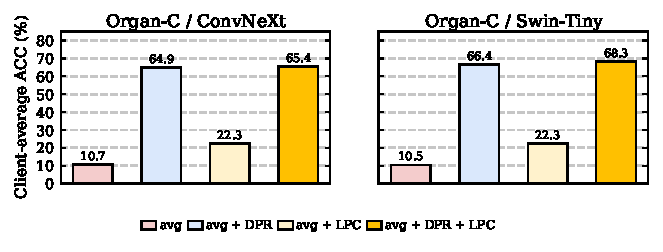
\includegraphics[width=\columnwidth]{figures/03_baseline_2x2_ablation.pdf}
\caption{\textbf{Module interaction on Organ-C.} We compare head averaging, DPR, LPC, and DPR+LPC on ConvNeXt and Swin-Tiny. DPR provides the primary gain, while adding LPC further improves DPR on both backbones.}
\label{fig:baseline-2x2-ablation}
\end{figure}

\subsection{Comparison with Existing Merging Methods}

% The main comparison uses client-average ACC: for each fixed dataset, model, and client number, we first average over the three $\beta$ skew levels and then compare merging methods. A cell is counted as successful when LAMP-Merge is greater than or equal to the strongest non-LAMP baseline in that cell.

Tables~\ref{tab:client-avg-swin-tiny}--\ref{tab:client-avg-vit-tiny} report four datasets. Against the eleven parameter-merging baselines, LAMP-Merge retains the highest dataset-level average ACC and Macro-F1 for each reported backbone--dataset pair. The additional supervised Pscore-MLP comparator provides a stronger comparison and wins in some settings. Across all five datasets and all 180 configurations, LAMP-Merge obtains 62.23\% ACC / 52.82\% Macro-F1 versus 56.00\% / 40.12\% for Pscore-MLP. On Derma, Pscore-MLP has higher mean ACC (67.89\% versus 62.40\%) but lower Macro-F1 (17.77\% versus 28.23\%), illustrating that accuracy alone does not establish broad class discrimination. This aggregate trade-off has exceptions: Pscore-MLP exceeds LAMP-Merge on both metrics for ResNet--Derma (68.10\% / 17.50\% versus 67.60\% / 15.04\%) and ViT-Tiny--Organ-C (63.12\% / 59.19\% versus 58.49\% / 57.06\%). On ViT-Tiny--Organ-S it also has higher ACC (58.02\% versus 54.52\%), with similar Macro-F1 (52.11\% versus 52.24\%). Thus, the overall advantage does not imply dominance in every configuration. The gain lines in the main tables include Pscore-MLP when identifying the strongest baseline, and negative gains are retained.


% \setcounter{dbltopnumber}{4}
% \setcounter{topnumber}{4}
% \setcounter{totalnumber}{4}


\subsection{Ablation Study}



\subsubsection{Module interaction.}
We compare head averaging, DPR, LPC, and DPR+LPC on Organ-C (Fig.~\ref{fig:baseline-2x2-ablation}). DPR raises ACC from 10.7\% to 64.9\% on ConvNeXt and 10.5\% to 66.4\% on Swin-Tiny, supplying the main recovery of diagnostic coverage. LPC alone reaches only 22.3\% on both backbones, but added on top of DPR it further raises ACC to 65.4\% and 68.3\%, a smaller but consistent complementary gain.



\subsubsection{Effectiveness of DPR}
We assess DPR from two axes. The \textbf{prototype semantics} axis replaces the class prototype: CHA uses the local classifier-head direction, GFM reuses one class-agnostic feature mean for all classes, SSH fills the normalized-weight head with a random unit vector, and SLP permutes prototypes across labels. The \textbf{client-support weighting} axis alters how observing clients are credited: UCW weights every observing client equally, whereas GCSW weights clients by total size rather than class-specific support. BSO is a separate cross-module count control that replaces class counts by presence indicators in both DPR and LPC.


\begin{table}[!t]
\centering
\caption{\textbf{Internal ablations of class evidence and count usage.} ACC / Macro-F1 (\%) over five datasets. Perturbing prototype semantics is substantially more damaging than changing support weights; LAMP-Merge attains the highest dataset-average ACC and Macro-F1.}
\label{tab:diagnostic-internal-ablation}
\scriptsize
\renewcommand{\arraystretch}{1.1}
\setlength{\tabcolsep}{2.4pt}
\resizebox{\columnwidth}{!}{%
\begin{tabular}{clccccc:c}
\noalign{\hrule height 1.25pt}
\rowcolor[HTML]{F2F2F2}
\textbf{Category} & \textbf{Setting} & \textbf{Blood} & \textbf{Derma} & \textbf{Organ-C} & \textbf{Organ-S} & \textbf{US} & \textbf{Avg} \\
\hline \hline
\multirow{4}{*}{\shortstack{Prototype\\semantics}} & CHA & 18.95 / 7.94 & 56.14 / 12.15 & 17.74 / 8.78 & 18.88 / 8.47 & 16.43 / 9.36 & 25.63 / 9.34 \\
& \cellcolor{gray!10}GFM & \cellcolor{gray!10}8.88 / 1.66 & \cellcolor{gray!10}66.88 / 11.45 & \cellcolor{gray!10}22.33 / 3.32 & \cellcolor{gray!10}23.54 / 3.46 & \cellcolor{gray!10}10.87 / 2.45 & \cellcolor{gray!10}26.50 / 4.47 \\
& SSH & 11.62 / 5.87 & 17.29 / 7.57 & 7.08 / 4.55 & 7.74 / 4.11 & 10.69 / 6.77 & 10.89 / 5.77 \\
& \cellcolor{gray!10}SLP & \cellcolor{gray!10}24.46 / 20.36 & \cellcolor{gray!10}28.73 / 11.39 & \cellcolor{gray!10}14.18 / 10.77 & \cellcolor{gray!10}16.25 / 9.64 & \cellcolor{gray!10}14.25 / 13.33 & \cellcolor{gray!10}19.57 / 13.10 \\
\hdashline
\multirow{2}{*}{\shortstack{DPR support\\weighting}} & UCW & 78.03 / 75.93 & 59.61 / 26.12 & 58.36 / 53.97 & 53.86 / 47.17 & 41.79 / 38.91 & 58.33 / 48.42 \\
& \cellcolor{gray!10}GCSW & \cellcolor{gray!10}78.45 / 76.13 & \cellcolor{gray!10}62.48 / 25.84 & \cellcolor{gray!10}59.11 / 54.55 & \cellcolor{gray!10}53.79 / 46.79 & \cellcolor{gray!10}43.13 / 40.38 & \cellcolor{gray!10}59.39 / 48.74 \\
\hdashline
\shortstack{Count control} & BSO & 78.03 / 75.93 & 44.96 / 27.03 & 57.86 / 54.69 & 53.24 / 48.56 & 41.79 / 38.91 & 55.18 / 49.02 \\
\hline \hline
& \cellcolor[HTML]{FFF9C4}\textbf{LAMP} & \cellcolor[HTML]{FFF9C4}\textbf{81.81 / 80.22} & \cellcolor[HTML]{FFF9C4}\textbf{62.40 / 28.25} & \cellcolor[HTML]{FFF9C4}\textbf{63.05 / 59.71} & \cellcolor[HTML]{FFF9C4}\textbf{57.67 / 52.28} & \cellcolor[HTML]{FFF9C4}\textbf{46.11 / 43.60} & \cellcolor[HTML]{FFF9C4}\textbf{62.21 / 52.81} \\
\noalign{\hrule height 1.25pt}
\end{tabular}
}
\end{table}

\begin{table}[!t]
\centering
\caption{\textbf{Internal ablation of LPC.} ACC / Macro-F1 (\%) over five datasets. LAMP-Merge attains the highest average ACC, while UPP exposes an ACC--Macro-F1 trade-off when the observed prior is removed.}
\label{tab:prevalence-internal-ablation}
\scriptsize
\renewcommand{\arraystretch}{1.1}
\setlength{\tabcolsep}{2.4pt}
\resizebox{\columnwidth}{!}{%
\begin{tabular}{lccccc:c}
\noalign{\hrule height 1.25pt}
\rowcolor[HTML]{F2F2F2}
\textbf{Setting} & \textbf{Blood} & \textbf{Derma} & \textbf{Organ-C} & \textbf{Organ-S} & \textbf{US} & \textbf{Avg} \\
\hline \hline
UPP & 81.81 / 80.22 & 46.58 / 29.33 & 62.57 / 60.35 & 57.50 / 54.10 & 46.11 / 43.60 & 58.91 / 53.52 \\

\rowcolor{gray!10}
AOC & 80.60 / 77.78 & 62.40 / 28.23 & 63.05 / 59.71 & 57.67 / 52.31 & 45.80 / 41.76 & 61.90 / 51.96 \\
CBP & 81.36 / 79.41 & 49.61 / 28.90 & 62.10 / 59.32 & 57.12 / 52.75 & 44.76 / 41.60 & 58.99 / 52.40 \\
\hline \hline
\rowcolor[HTML]{FFF9C4}
\textbf{LAMP-Merge} & \textbf{81.81 / 80.22} & \textbf{62.40 / 28.25} & \textbf{63.05 / 59.71} & \textbf{57.67 / 52.28} & \textbf{46.11 / 43.60} & \textbf{62.21 / 52.81} \\
\noalign{\hrule height 1.25pt}
\end{tabular}
}
\end{table}


% Table~\ref{tab:diagnostic-internal-ablation} and Fig.~\ref{fig:internal_module_ablations}
Table~\ref{tab:diagnostic-internal-ablation} shows every replacement lowers the \textbf{dataset-average ACC}. Corrupting prototype semantics is most damaging: overall ACC / Macro-F1 falls from \textbf{62.21\%/52.81\%} to as low as \textbf{10.89\%/5.77\%} (\textcolor{DropRed}{51.32/47.04 pp}). Altering DPR's support weights is less destructive, yet the stronger DPR-only variant still trails by \textcolor{DropRed}{2.82/4.07 pp}. BSO drops further but jointly changes DPR and LPC, only evidencing count magnitude across the pipeline. Derma shows why both metrics matter: GFM's high ACC with 11.45\% Macro-F1 signals dominant-class concentration, not broad discrimination. Thus DPR needs both aligned prototypes and support weighting.


\subsubsection{Effectiveness of LPC}


% \begin{figure}[!t]
%     \centering
%     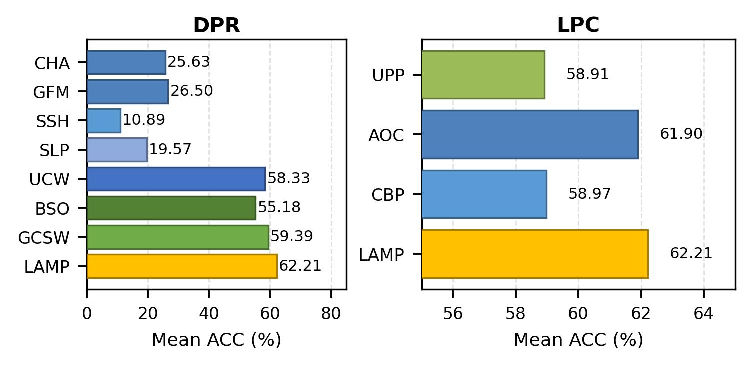
\includegraphics[width=\columnwidth]{figures/02_internal_module_ablations.pdf}
%     \caption{\textbf{Every internal variant of DPR and LPC falls below the full model.} Visual companion to Tables~\ref{tab:diagnostic-internal-ablation} and~\ref{tab:prevalence-internal-ablation}; plotted abbreviations are defined in the ablation text above. No single component can be removed without loss, confirming that the two modules are jointly necessary.}

%     \label{fig:internal_module_ablations}
% \end{figure}

We test three controls for LPC. Two probe the \textbf{prior estimator}: UPP replaces the observed class distribution with a flat prior, and CBP averages each client's normalized prevalence with equal weight instead of by sample count. AOC probes the \textbf{activation gate} by applying the prior to every configuration.

%Table~\ref{tab:prevalence-internal-ablation} and Fig.~\ref{fig:internal_module_ablations} 
Table~\ref{tab:prevalence-internal-ablation} shows all three controls reduce average ACC from \textbf{62.21\%}: UPP and CBP lose 3.30 and 3.22 pp, AOC 0.31 pp. UPP raises Macro-F1 from 52.81\% to 53.52\%, the expected trade-off: flattening the prior favors class-balanced performance but sacrifices accuracy under the long tail, while removing the gate loses 0.85 Macro-F1 pp. Gated calibration thus gives a better ACC--Macro-F1 balance than applying the prior everywhere.

\subsubsection{Unaveraged client-count and skew results}
Table~\ref{tab:swin-full-grid} reports every $K\times\beta$ setting for Swin-Tiny, including Organ-S, without averaging over either axis. Swin-Tiny is selected by the highest LAMP-Merge mean ACC over all five datasets and all nine settings: 63.97\%, compared with 62.62\% for ConvNeXt, 61.57\% for ResNet, and 60.75\% for ViT-Tiny. This explicit, retrospective selection provides a compact descriptive view of the strongest backbone; the single-seed results do not quantify run-to-run uncertainty.
\begin{table*}[!t]
\centering
\small
\caption{Unaveraged LAMP-Merge test ACC / Macro-F1 (\%) on Swin-Tiny. Each cell is one run (seed 42); no averaging over $K$ or $\beta$. US denotes ChaoShengMNIST.}
\label{tab:swin-full-grid}
\setlength{\tabcolsep}{7pt}
\begin{tabular}{cc|ccccc}
\hline
$K$ & $\beta$ & Blood & Derma & Organ-C & Organ-S & US \\
\hline
3 & 0 & 77.55 / 75.92 & 63.34 / 28.26 & 68.42 / 65.70 & 62.77 / 58.44 & 48.34 / 46.50 \\
3 & 0.01 & 77.55 / 75.90 & 63.34 / 28.30 & 68.51 / 65.83 & 62.60 / 58.20 & 48.25 / 46.37 \\
3 & 0.1 & 77.52 / 76.02 & 63.04 / 27.71 & 68.54 / 65.99 & 62.35 / 57.98 & 46.54 / 44.43 \\
\hline
5 & 0 & 77.55 / 75.92 & 63.34 / 28.26 & 68.42 / 65.70 & 62.77 / 58.44 & 48.34 / 46.50 \\
5 & 0.01 & 77.46 / 75.85 & 62.89 / 27.89 & 68.54 / 65.85 & 62.77 / 58.45 & 48.61 / 46.93 \\
5 & 0.1 & 77.32 / 75.54 & 63.29 / 28.57 & 67.55 / 64.59 & 62.84 / 58.45 & 49.15 / 47.15 \\
\hline
7 & 0 & 77.55 / 75.92 & 63.34 / 28.26 & 68.42 / 65.70 & 62.77 / 58.44 & 48.34 / 46.50 \\
7 & 0.01 & 77.49 / 75.97 & 63.09 / 27.44 & 68.00 / 65.13 & 62.89 / 58.53 & 48.52 / 46.71 \\
7 & 0.1 & 76.85 / 75.12 & 62.84 / 26.87 & 67.95 / 65.00 & 62.85 / 58.20 & 48.34 / 46.59 \\
\hline
\end{tabular}
\end{table*}




\begin{table}[!t]
\centering
\caption{\textbf{Prediction-collapse diagnostics over five datasets.} Relative to the strongest original non-LAMP reference for each metric (excluding the separately evaluated supervised Pscore-MLP comparator), LAMP-Merge lowers prediction concentration and predicted--true total variation while increasing the effective number of predicted classes.}
\label{tab:collapse-key}
\scriptsize
\setlength{\tabcolsep}{2.2pt}
\renewcommand{\arraystretch}{1.0}
\resizebox{\columnwidth}{!}{%
\begin{tabular}{clccccc:c}
\noalign{\hrule height 1.25pt}
\rowcolor[HTML]{F2F2F2}
\textbf{Metric} & \textbf{Series} & \textbf{Blood} & \textbf{Derma} & \textbf{Organ-C} & \textbf{Organ-S} & \textbf{US} & \textbf{Avg} \\
\hline \hline
 & \cellcolor{gray!10}Best ref. & \cellcolor{gray!10}80.20 & \cellcolor{gray!10}85.18 & \cellcolor{gray!10}72.38 & \cellcolor{gray!10}71.12 & \cellcolor{gray!10}80.31 & \cellcolor{gray!10}79.02 \\
\multirow{-2}{*}{Collapse (\%) $\downarrow$} & \cellcolor[HTML]{FFF9C4}\textbf{LAMP} & \cellcolor[HTML]{FFF9C4}\textbf{19.58} & \cellcolor[HTML]{FFF9C4}\textbf{68.05} & \cellcolor[HTML]{FFF9C4}\textbf{20.72} & \cellcolor[HTML]{FFF9C4}\textbf{24.36} & \cellcolor[HTML]{FFF9C4}\textbf{20.45} & \cellcolor[HTML]{FFF9C4}\textbf{30.63} \\
\hdashline
 & \cellcolor{gray!10}Best ref. & \cellcolor{gray!10}1.81 & \cellcolor{gray!10}1.65 & \cellcolor{gray!10}2.49 & \cellcolor{gray!10}2.53 & \cellcolor{gray!10}1.98 & \cellcolor{gray!10}2.05 \\
\multirow{-2}{*}{Eff. classes $\uparrow$} & \cellcolor[HTML]{FFF9C4}\textbf{LAMP} & \cellcolor[HTML]{FFF9C4}\textbf{7.48} & \cellcolor[HTML]{FFF9C4}\textbf{3.10} & \cellcolor[HTML]{FFF9C4}\textbf{9.55} & \cellcolor[HTML]{FFF9C4}\textbf{8.44} & \cellcolor[HTML]{FFF9C4}\textbf{7.44} & \cellcolor[HTML]{FFF9C4}\textbf{7.20} \\
\hdashline
 & \cellcolor{gray!10}Best ref. & \cellcolor{gray!10}73.48 & \cellcolor{gray!10}46.03 & \cellcolor{gray!10}75.42 & \cellcolor{gray!10}73.85 & \cellcolor{gray!10}72.73 & \cellcolor{gray!10}69.44 \\
\multirow{-2}{*}{Pred-true TV (\%) $\downarrow$} & \cellcolor[HTML]{FFF9C4}\textbf{LAMP} & \cellcolor[HTML]{FFF9C4}\textbf{3.97} & \cellcolor[HTML]{FFF9C4}\textbf{17.09} & \cellcolor[HTML]{FFF9C4}\textbf{12.38} & \cellcolor[HTML]{FFF9C4}\textbf{13.17} & \cellcolor[HTML]{FFF9C4}\textbf{15.51} & \cellcolor[HTML]{FFF9C4}\textbf{12.42} \\
\noalign{\hrule height 1.25pt}
\end{tabular}
}
\end{table}


\begin{figure}[!t]
\centering
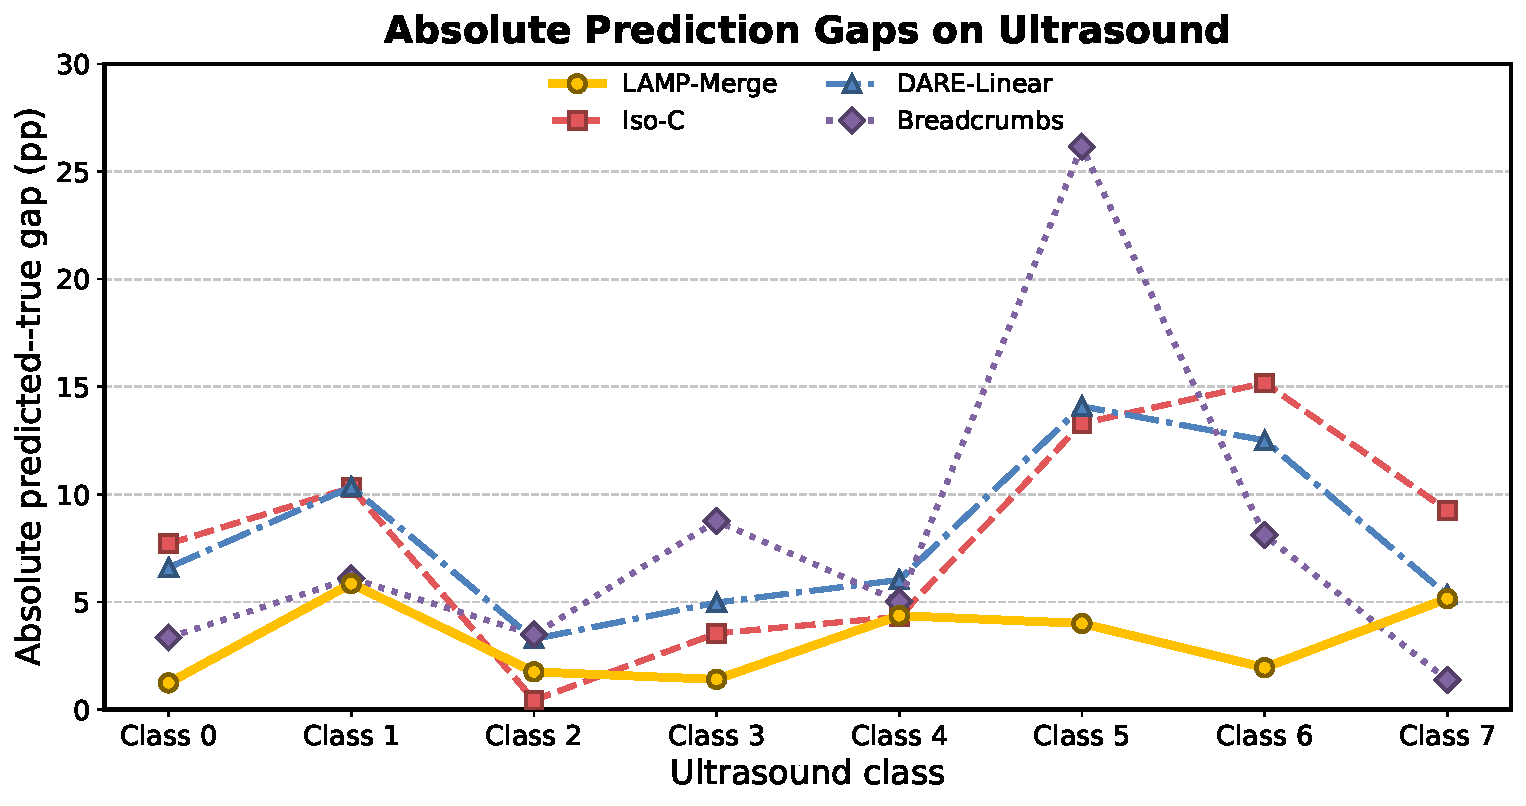
\includegraphics[width=0.78\linewidth]{figures/04_ultrasound_class_distribution.pdf}
\caption{\textbf{Absolute predicted--true class-frequency gaps on Ultrasound.} LAMP-Merge reduces the gap on most classes relative to Iso-C, DARE-Linear, and Breadcrumbs, especially for classes~5 and~6.}
\label{fig:visual-chaosheng_predict}
\end{figure}

\subsection{Prediction-Collapse Diagnostics}
We additionally report \textbf{collapse ratio, effective predicted classes, and predicted--true total variation}. With $q_c$ and $\bar{q}_c$ the predicted and true class distributions over the test set, the three diagnostics are
\begin{equation}
\begin{array}{c}
\rho=\max_c q_c,\qquad C_{\mathrm{eff}}=\exp\left(-\sum_c q_c\log q_c\right),\\[3pt]
\mathrm{TV}(q,\bar{q})=\frac{1}{2}\sum_c|q_c-\bar{q}_c|.
\end{array}
\end{equation}
Lower $\rho$ indicates less single-class concentration, while higher $C_{\mathrm{eff}}$ indicates broader predicted-class coverage. 
%Because a long-tailed true distribution may itself have a large dominant-class share, we interpret both jointly with TV rather than treating a small $\rho$ as sufficient evidence of correct calibration.


Table~\ref{tab:collapse-key} shows LAMP-Merge reduces the average collapse ratio from 79.02\% to 30.63\%, raises the effective class count from 2.05 to 7.20, and reduces predicted--true TV from 69.44\% to 12.42\%. Derma stays more concentrated, but its 68.05\% collapse ratio is close to the 66.9\% majority share in the true test distribution. The gains thus arise from broader diagnostic coverage rather than a more aggressive majority-class predictor.

\subsection{Distribution Analysis}

Examining the absolute per-class gap between predicted and true class frequencies on Ultrasound (Fig.~\ref{fig:visual-chaosheng_predict}), LAMP-Merge produces smaller gaps on most classes, clearest on classes~5 and~6, while retaining nonzero deviations that reflect residual calibration error.




\begin{figure}[!t]
\centering
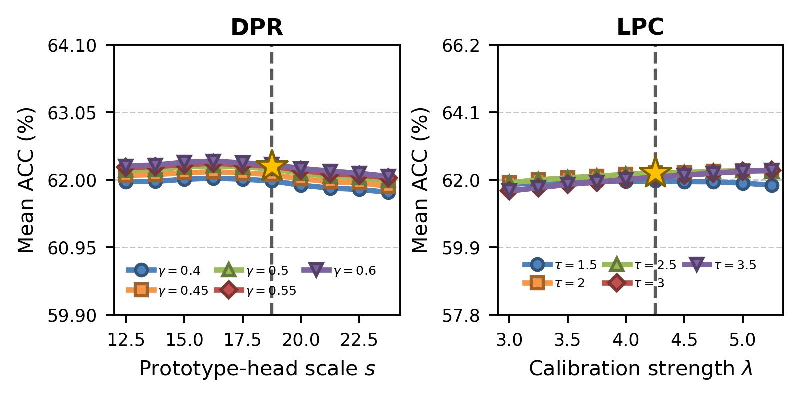
\includegraphics[width=\columnwidth]{figures/05_hyperparameter_sensitivity.pdf}
\caption{\textbf{Sensitivity to $\gamma$, $s$, $\tau$, and $\lambda$.} Full-scope averages over all datasets; each curve fixes one module parameter and scans the other. The selected configuration lies within a broad high-performing region.}
\label{fig:hparam-analysis}
\end{figure}

\begin{figure}[!t]
\centering
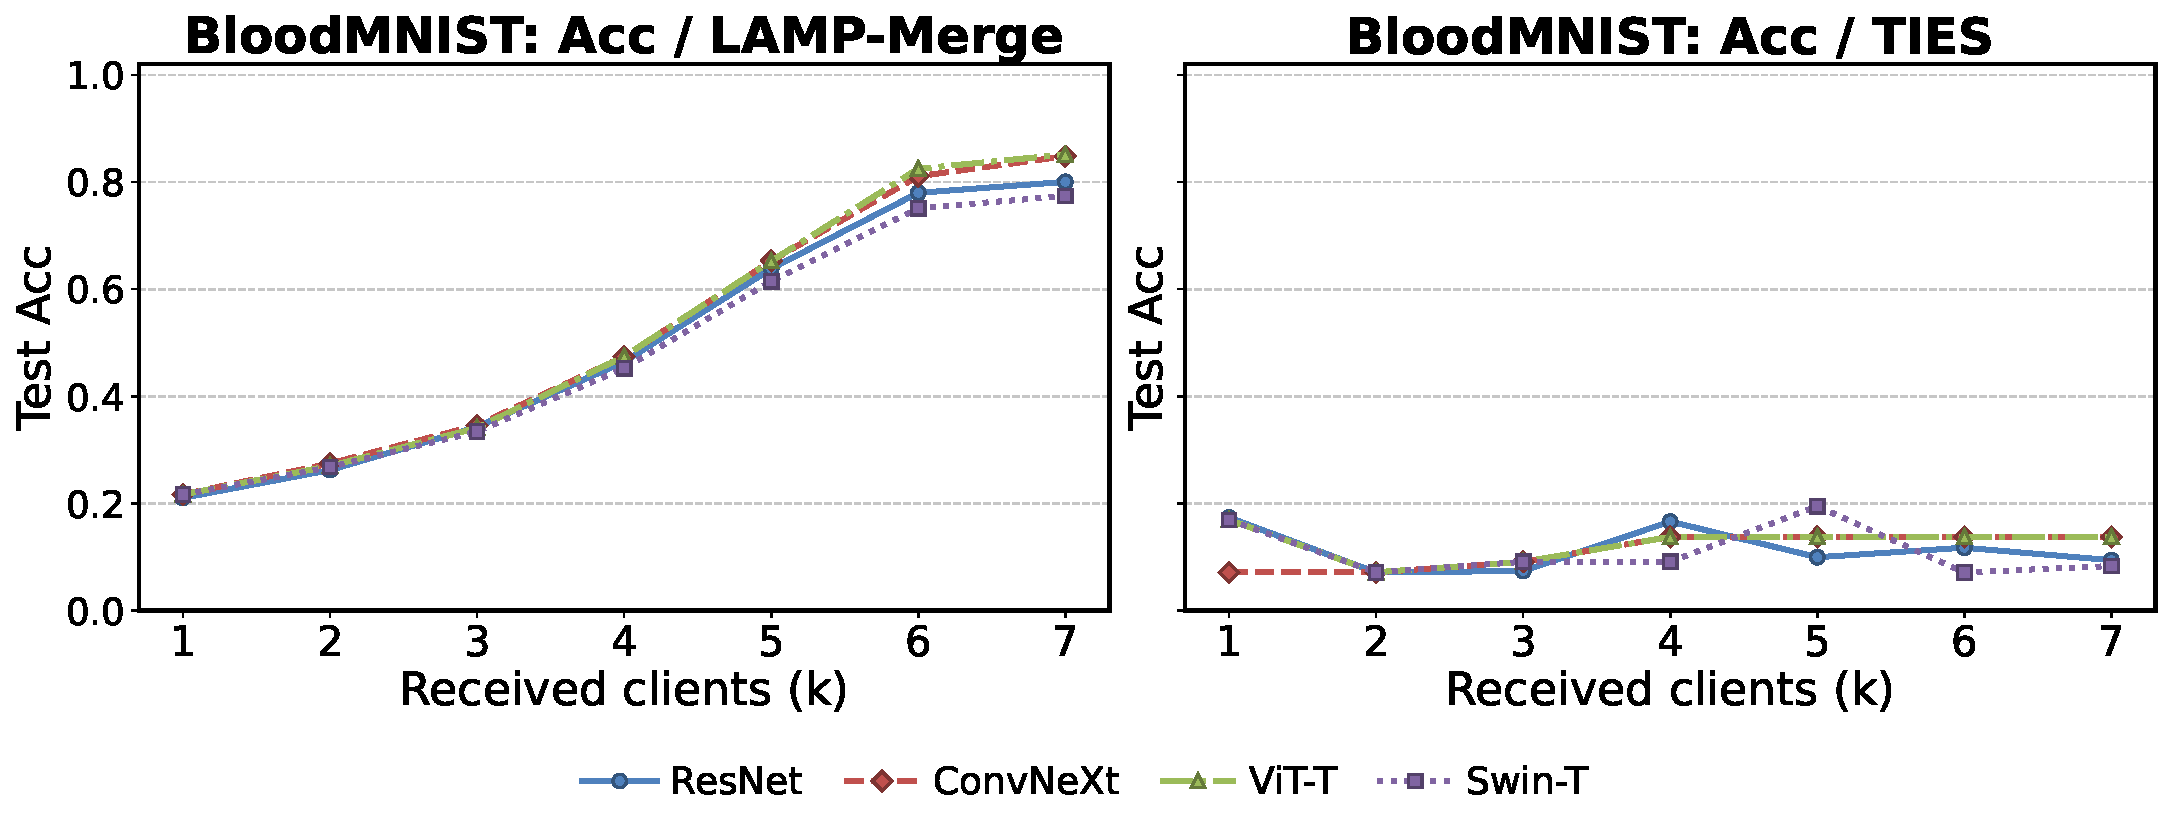
\includegraphics[width=0.85\linewidth]{figures/ties_vs_lamp_merge_blood_acc_k1_to_k7.pdf}
\caption{\textbf{Asynchronous incremental merging on BloodMNIST.} Test accuracy as the seven clients arrive one at a time, for all four backbones. LAMP-Merge (left) improves monotonically, while TIES (right) stays flat and low.}
\label{fig:async-bloodmnist}
\end{figure}

\subsection{Asynchronous Incremental Merging}
Merging the seven BloodMNIST clients one at a time as they arrive, across all four backbones (Fig.~\ref{fig:async-bloodmnist}), LAMP-Merge \textbf{raises test accuracy monotonically as clients accumulate}, so a usable model is available at every step and keeps improving with each new arrival. TIES, by contrast, \textbf{stays flat and low throughout}, as a generic parameter-space merge cannot turn incremental arrivals into progressive gains.

\subsection{Hyperparameter Sensitivity}
Fig.~\ref{fig:hparam-analysis} varies DPR's prototype-head scale $s$ under several $\gamma$ values and LPC's calibration strength $\lambda$ under several $\tau$ values. The two recorded grids each contain 50 points, each evaluated over 180 configurations (five datasets, four backbones, and nine $K\times\beta$ settings). DPR scans $\gamma\in\{0.40,0.45,0.50,0.55,0.60\}$ and $s=12.50,13.75,\ldots,23.75$; LPC scans $\tau\in\{1.5,2.0,2.5,3.0,3.5\}$ and $\lambda=3.00,3.25,\ldots,5.25$, keeping the other module at its selected setting.

The common choice $\gamma=0.55$, $s=18.75$, $\tau=2.5$, $\lambda=4.25$ is an interior operating point used without dataset-specific tuning. Sublinear $\gamma$ tempers support dominance; $s$ controls the prototype-score magnitude relative to the LPC bias; $\tau$ limits prior adjustment to pronounced imbalance; and $\lambda$ controls its strength. The recorded mean ACC is 62.2065\% at this setting. Across the DPR grid, ACC ranges from 61.8023\% to 62.2890\%; the maximum at $(\gamma,s)=(0.60,16.25)$ exceeds the selected setting by only 0.0825 pp. Across the LPC grid, the range is 61.6468\%--62.2971\%, with the maximum at $(\tau,\lambda)=(3.0,5.25)$ only 0.0906 pp higher. These observations support a stable operating region, not unique optimality or a theoretical derivation of the numerical constants.

The archived sweeps evaluate the test split and are retrospective sensitivity analyses. They do not establish test-independent hyperparameter selection; selection on a separate validation set and multi-seed confirmation remain necessary for an unbiased prospective assessment.


\section{Conclusion}

We study medical model merging under a raw-data-free protocol. Generic parameter-space merging collapses when hospitals cover different diagnostic classes, while an observed long-tailed prior makes collapse correction different from enforcing uniform predictions. LAMP-Merge addresses these coupled problems by \textbf{reconstructing diagnostic class directions} from client-side prototypes and calibrating the classifier with empirical class statistics, improving both ACC and Macro-F1.

Our conclusions are limited to head-only synthesis in a shared frozen feature space. Identical feature coordinates are essential for direct prototype aggregation; independently fine-tuned encoders are unsupported without an additional representation-alignment mechanism, which would change the method. The reconstructed benchmark partitions isolate label skew through disjoint within-class sampling and do not establish robustness to real hospital acquisition shifts. Uploaded counts recover the participating samples' empirical prior, not population prevalence or exact predicted frequencies. Keeping raw images local reduces direct data exposure, but aggregate statistics are not a formal privacy guarantee; no differential privacy, secure aggregation, or attack-resistance evaluation is provided. Single-seed evaluation, retrospective test-set sensitivity grids, and unequal information interfaces across baselines further limit the claims. Real multicenter validation, independently validated hyperparameter selection, and explicit privacy mechanisms remain future work.


\bibliographystyle{IEEEtran}
\bibliography{aaai2026}
% \appendix
% \def\appendixinmain{}
% \ifdefined\appendixinmain
\else
\PassOptionsToPackage{table}{xcolor}
\documentclass[letterpaper]{article}
\usepackage[submission]{aaai2026}
\usepackage{times}
\usepackage{helvet}
\usepackage{courier}
\usepackage[hyphens]{url}
\usepackage{graphicx}
\usepackage{natbib}
\usepackage{caption}
\usepackage{amsmath}
\usepackage{amssymb}
\usepackage{amsthm}
\usepackage{algorithm}
\usepackage{algorithmic}
\usepackage[table]{xcolor}
\usepackage{multirow}
\usepackage{arydshln}
\usepackage{placeins}
\frenchspacing
\setlength{\pdfpagewidth}{8.5in}
\setlength{\pdfpageheight}{11in}
\setcounter{secnumdepth}{3} % number appendix sections so cross-references resolve

% Theorem-like environments for the analysis section.
\theoremstyle{definition}
\newtheorem{assumption}{Assumption}
\theoremstyle{plain}
\newtheorem{proposition}{Proposition}
\newtheorem{lemma}{Lemma}

\title{Supplementary Material\\[2pt]
\large LAMP-Merge: Long-tail-Aware Medical Prototype Merging\\
for One-shot Asynchronous Clinical Models}
\author{}
\date{}

\begin{document}
\maketitle
\appendix
\newcommand{\appendixstandalonefooter}{\bibliography{aaai2026}\end{document}}
\fi
\ifdefined\appendixinmain
\newcommand{\appendixstandalonefooter}{}
\fi

\section{Overview of the Supplementary Material}

This supplement is intended to make the empirical and theoretical claims in the paper reproducible without repeating the main exposition. It contains four types of material. First, Section~\ref{app:algorithm} gives an executable-level specification of LAMP-Merge, emphasizing the boundary between local hospital computation and server-side merging. Second, Sections~\ref{app:organ-s-results} and~\ref{app:datasets} provide additional experimental context: the full Organ-S results omitted from the compact main tables, and the class-wise dataset statistics used to construct the reported client splits. Third, Section~\ref{app:ablation-configurations} defines every internal ablation by the exact mathematical substitution applied to the full method, so that each ablation tests a single modeling choice. Finally, Sections~\ref{app:theory}--\ref{app:repro} provide supporting theory, metric definitions, and hyperparameter-sweep details required for reproduction and checklist verification.

Unless otherwise stated, \(K\) denotes the number of clients, \(C\) denotes the number of diagnosis classes, \(n_{i,c}\) denotes the support count of class \(c\) on client \(i\), \(m_{i,c}\) denotes the corresponding prevalence count, and \(\phi_0(T(\cdot))\) denotes the frozen reference encoder applied after the evaluation transform \(T\).

\section{Algorithmic Specification}
\label{app:algorithm}

Algorithm~\ref{app:alg:lamp} provides the procedural specification corresponding to the method section of the paper. It is included here to clarify the execution order and the information boundary, rather than to introduce an additional variant of LAMP-Merge. The inputs are the local datasets \(\{D_i\}_{i=1}^{K}\), the shared frozen reference encoder \(\phi_0\), the evaluation transform \(T\), and four scalar hyperparameters \(\gamma,s,\tau,\lambda\). The output is a single merged diagnostic model \(\theta_m=(\phi_0,\{w_c,b_c\}_{c=1}^{C})\).

The algorithm separates local statistic construction from server-side merging. Lines~1--6 are executed independently by each hospital. Client \(i\) computes the class prototype \(\mu_{i,c}\), support count \(n_{i,c}\), and prevalence count \(m_{i,c}\) for every observed diagnosis class. The upload contains only these class-level statistics. Lines~7--20 are executed once on the server. The server first reconstructs a class-specific prototype \(p_c\) through support-aware aggregation and then converts it into the classifier weight \(w_c\). The prevalence counts are used only to form the gated centered log-prior \(b_c\). Thus, the merged model is obtained in one pass, without raw-image transfer, gradient exchange, or additional local optimization after the upload.

\begin{algorithm}[!t]
\caption{LAMP-Merge}
\label{app:alg:lamp}
\begin{algorithmic}[1]
\REQUIRE Clients $\{D_i\}_{i=1}^{K}$; frozen reference encoder $\phi_0$; transform $T$; hyperparameters $\gamma,s,\tau,\lambda$
\ENSURE Merged diagnostic model $\theta_m=(\phi_0,\{w_c,b_c\}_{c=1}^{C})$
\STATE \textbf{Hospital side} (each client $i$, uploaded once):
\FOR{each class $c=1,\dots,C$}
    \STATE $n_{i,c}\leftarrow |D_{i,c}|$;\quad $m_{i,c}\leftarrow$ local label count of class $c$
    \STATE $\mu_{i,c}\leftarrow \frac{1}{n_{i,c}}\sum_{(x,y)\in D_i}\mathbf{1}[y=c]\,\phi_0(T(x))$ \quad\textbf{if } $n_{i,c}>0$
\ENDFOR
\STATE upload $\{(\mu_{i,c},n_{i,c},m_{i,c})\}_{c=1}^{C}$; \textbf{raw images stay local}
\STATE \textbf{Merging} (single pass):
\FOR{each class $c=1,\dots,C$}
    \STATE $e_{i,c}\leftarrow (n_{i,c}+1)^{\gamma}\,\mathbf{1}[n_{i,c}>0]$ for all $i$
    \STATE $\alpha_{i,c}\leftarrow e_{i,c}\big/\sum_{j=1}^{K} e_{j,c}$
    \STATE $p_c\leftarrow \sum_{i=1}^{K}\alpha_{i,c}\,\mu_{i,c}$ \hfill $\triangleright$ DPR fusion
    \STATE $w_c\leftarrow s\,p_c/\|p_c\|_2$
\ENDFOR
\STATE $\pi_c\leftarrow \sum_{i} m_{i,c}\big/\sum_{k}\sum_{i} m_{i,k}$;\quad $r\leftarrow C\max_c \pi_c$
\IF{$r>\tau$}
    \STATE $b_c\leftarrow \lambda\big(\log\pi_c-\frac{1}{C}\sum_{k}\log\pi_k\big)$ for all $c$ \hfill $\triangleright$ LPC
\ELSE
    \STATE $b_c\leftarrow 0$ for all $c$
\ENDIF
\RETURN $\theta_m=(\phi_0,\{w_c,b_c\}_{c=1}^{C})$
\end{algorithmic}
\end{algorithm}

The algorithm also specifies the privacy and communication assumptions used throughout the experiments. The client upload is \(\{(\mu_{i,c},n_{i,c},m_{i,c})\}_{c=1}^{C}\); it does not contain raw images, sample identities, gradients, or a server-side validation set. Once these statistics and the hyperparameters are fixed, the server-side computation is deterministic. This makes the merge reproducible from the uploaded statistics alone and distinguishes the setting from multi-round federated optimization.

\section{Additional Organ-S Results}
\label{app:organ-s-results}

The main paper reports the compact set of benchmark tables required to compare methods across model families. To keep the main body readable, the Organ-S table is moved to this supplement while preserving the same evaluation protocol, the same client counts, and the same reporting format. Tables~\ref{tab:appendix-organs-swin}--\ref{tab:appendix-organs-vit} report client-average ACC / Macro-F1 in percentage points. \textbf{Across all four backbones, LAMP-Merge remains the strongest method on Organ-S, confirming that the conclusion does not depend on omitting this CT view from the compact main tables.}

\begin{table}[!t]
\centering
\caption{Organ-S client-average test ACC / Macro-F1 (\%) on Swin-Tiny.}
\label{tab:appendix-organs-swin}
\scriptsize
\renewcommand{\arraystretch}{1.18}
\setlength{\tabcolsep}{3.2pt}
\resizebox{\columnwidth}{!}{%
\begin{tabular}{lcccc}
\noalign{\hrule height 1.25pt}
\rowcolor[HTML]{F2F2F2}
\textbf{Method} & \textbf{$K=3$} & \textbf{$K=5$} & \textbf{$K=7$} & \textbf{Avg} \\
\hline \hline
Weight Avg. & 23.05 / 12.58 & 17.70 / 9.52 & 19.07 / 10.37 & 19.94 / 10.82 \\
\rowcolor{gray!10} TIES & 14.68 / 8.88 & 14.03 / 9.87 & 15.91 / 10.90 & 14.87 / 9.88 \\
DARE-Linear & 20.61 / 11.41 & 16.22 / 9.41 & 15.52 / 8.33 & 17.45 / 9.72 \\
\rowcolor{gray!10} DARE-TIES & 14.24 / 8.21 & 12.98 / 8.61 & 11.15 / 7.05 & 12.79 / 7.96 \\
RegMean & 20.04 / 10.36 & 20.95 / 9.04 & 19.66 / 10.78 & 20.22 / 10.06 \\
\rowcolor{gray!10} Fisher & 18.47 / 11.70 & 17.36 / 8.75 & 20.49 / 10.35 & 18.77 / 10.27 \\
Breadcrumbs & 17.67 / 10.96 & 12.37 / 8.14 & 11.13 / 7.21 & 13.72 / 8.77 \\
\rowcolor{gray!10} Model Stock & 21.86 / 12.85 & 17.11 / 9.26 & 17.15 / 8.73 & 18.71 / 10.28 \\
Iso-C & 25.18 / 15.34 & 22.82 / 10.93 & 18.34 / 10.30 & 22.12 / 12.19 \\
\rowcolor{gray!10} Free-Merging & 23.05 / 12.58 & 17.70 / 9.52 & 19.07 / 10.37 & 19.94 / 10.82 \\
RobustMerge & 17.85 / 10.64 & 16.22 / 10.64 & 15.42 / 8.45 & 16.50 / 9.91 \\
\rowcolor{gray!10} FROM & 18.11 / 10.16 & 17.43 / 9.56 & 12.89 / 7.62 & 16.14 / 9.11 \\
\hline \hline
\rowcolor[HTML]{FFF9C4}
\textbf{LAMP-Merge} & \textbf{62.58 / 58.21} & \textbf{62.80 / 58.45} & \textbf{62.84 / 58.39} & \textbf{62.74 / 58.35} \\
\noalign{\hrule height 1.25pt}
\end{tabular}
}
\end{table}

\begin{table}[!t]
\centering
\caption{Organ-S client-average test ACC / Macro-F1 (\%) on ConvNeXt.}
\label{tab:appendix-organs-convnext}
\scriptsize
\renewcommand{\arraystretch}{1.18}
\setlength{\tabcolsep}{3.2pt}
\resizebox{\columnwidth}{!}{%
\begin{tabular}{lcccc}
\noalign{\hrule height 1.25pt}
\rowcolor[HTML]{F2F2F2}
\textbf{Method} & \textbf{$K=3$} & \textbf{$K=5$} & \textbf{$K=7$} & \textbf{Avg} \\
\hline \hline
Weight Avg. & 17.66 / 8.18 & 12.61 / 7.24 & 14.33 / 5.48 & 14.87 / 6.97 \\
\rowcolor{gray!10} TIES & 11.83 / 6.50 & 13.13 / 8.79 & 11.34 / 7.02 & 12.10 / 7.44 \\
DARE-Linear & 17.48 / 8.29 & 8.18 / 6.03 & 8.73 / 5.12 & 11.46 / 6.48 \\
\rowcolor{gray!10} DARE-TIES & 14.34 / 7.74 & 9.80 / 7.03 & 12.17 / 6.83 & 12.11 / 7.20 \\
RegMean & 15.71 / 9.76 & 13.87 / 7.28 & 16.55 / 6.68 & 15.37 / 7.91 \\
\rowcolor{gray!10} Fisher & 22.16 / 10.64 & 16.09 / 9.05 & 17.67 / 8.49 & 18.64 / 9.39 \\
Breadcrumbs & 9.86 / 6.89 & 7.97 / 6.03 & 8.10 / 5.06 & 8.64 / 5.99 \\
\rowcolor{gray!10} Model Stock & 15.72 / 7.26 & 10.61 / 7.02 & 11.48 / 5.24 & 12.60 / 6.50 \\
Iso-C & 16.66 / 8.25 & 12.72 / 8.92 & 14.98 / 6.69 & 14.79 / 7.95 \\
\rowcolor{gray!10} Free-Merging & 17.66 / 8.18 & 12.61 / 7.24 & 14.33 / 5.48 & 14.87 / 6.97 \\
RobustMerge & 13.57 / 6.67 & 6.79 / 5.45 & 7.52 / 4.47 & 9.29 / 5.53 \\
\rowcolor{gray!10} FROM & 16.19 / 7.85 & 14.36 / 6.72 & 11.94 / 5.65 & 14.16 / 6.74 \\
\hline \hline
\rowcolor[HTML]{FFF9C4}
\textbf{LAMP-Merge} & \textbf{60.55 / 56.06} & \textbf{60.50 / 56.07} & \textbf{60.66 / 56.09} & \textbf{60.57 / 56.07} \\
\noalign{\hrule height 1.25pt}
\end{tabular}
}
\end{table}

\begin{table}[!t]
\centering
\caption{Organ-S client-average test ACC / Macro-F1 (\%) on ResNet.}
\label{tab:appendix-organs-resnet}
\scriptsize
\renewcommand{\arraystretch}{1.18}
\setlength{\tabcolsep}{3.2pt}
\resizebox{\columnwidth}{!}{%
\begin{tabular}{lcccc}
\noalign{\hrule height 1.25pt}
\rowcolor[HTML]{F2F2F2}
\textbf{Method} & \textbf{$K=3$} & \textbf{$K=5$} & \textbf{$K=7$} & \textbf{Avg} \\
\hline \hline
Weight Avg. & 23.64 / 7.49 & 12.41 / 3.79 & 15.30 / 3.55 & 17.12 / 4.95 \\
\rowcolor{gray!10} TIES & 13.07 / 3.70 & 11.30 / 4.36 & 13.47 / 4.43 & 12.62 / 4.16 \\
DARE-Linear & 23.58 / 7.15 & 13.95 / 4.22 & 16.91 / 5.20 & 18.15 / 5.52 \\
\rowcolor{gray!10} DARE-TIES & 14.00 / 5.08 & 9.03 / 3.10 & 12.42 / 4.16 & 11.81 / 4.11 \\
RegMean & 20.27 / 9.88 & 9.12 / 4.70 & 11.81 / 5.89 & 13.73 / 6.82 \\
\rowcolor{gray!10} Fisher & 16.69 / 5.25 & 10.74 / 4.53 & 14.84 / 3.24 & 14.09 / 4.34 \\
Breadcrumbs & 13.20 / 7.20 & 12.05 / 4.78 & 11.83 / 4.58 & 12.36 / 5.52 \\
\rowcolor{gray!10} Model Stock & 23.48 / 7.35 & 12.63 / 4.26 & 15.25 / 3.61 & 17.12 / 5.07 \\
Iso-C & 25.31 / 10.64 & 10.91 / 5.37 & 13.97 / 4.49 & 16.73 / 6.83 \\
\rowcolor{gray!10} Free-Merging & 23.64 / 7.49 & 12.41 / 3.79 & 15.30 / 3.55 & 17.12 / 4.95 \\
RobustMerge & 19.44 / 6.52 & 10.32 / 4.39 & 11.86 / 4.03 & 13.87 / 4.98 \\
\rowcolor{gray!10} FROM & 16.73 / 4.99 & 12.10 / 3.48 & 12.30 / 3.11 & 13.71 / 3.86 \\
\hline \hline
\rowcolor[HTML]{FFF9C4}
\textbf{LAMP-Merge} & \textbf{52.98 / 42.87} & \textbf{52.79 / 42.54} & \textbf{52.81 / 42.32} & \textbf{52.86 / 42.58} \\
\noalign{\hrule height 1.25pt}
\end{tabular}
}
\end{table}

\begin{table}[!t]
\centering
\caption{Organ-S client-average test ACC / Macro-F1 (\%) on ViT-Tiny.}
\label{tab:appendix-organs-vit}
\scriptsize
\renewcommand{\arraystretch}{1.18}
\setlength{\tabcolsep}{3.2pt}
\resizebox{\columnwidth}{!}{%
\begin{tabular}{lcccc}
\noalign{\hrule height 1.25pt}
\rowcolor[HTML]{F2F2F2}
\textbf{Method} & \textbf{$K=3$} & \textbf{$K=5$} & \textbf{$K=7$} & \textbf{Avg} \\
\hline \hline
Weight Avg. & 10.06 / 6.70 & 12.16 / 5.80 & 9.20 / 3.47 & 10.47 / 5.32 \\
\rowcolor{gray!10} TIES & 8.67 / 4.89 & 13.92 / 3.58 & 10.29 / 4.46 & 10.96 / 4.31 \\
DARE-Linear & 8.96 / 5.43 & 13.59 / 4.62 & 13.99 / 5.57 & 12.18 / 5.20 \\
\rowcolor{gray!10} DARE-TIES & 8.21 / 5.67 & 13.62 / 5.14 & 10.75 / 5.48 & 10.86 / 5.43 \\
RegMean & 13.81 / 8.29 & 13.39 / 6.79 & 10.26 / 5.19 & 12.48 / 6.76 \\
\rowcolor{gray!10} Fisher & 12.43 / 6.85 & 13.30 / 6.28 & 10.96 / 5.10 & 12.23 / 6.08 \\
Breadcrumbs & 5.26 / 2.62 & 4.26 / 2.66 & 4.71 / 3.45 & 4.74 / 2.91 \\
\rowcolor{gray!10} Model Stock & 7.79 / 4.90 & 8.07 / 4.48 & 6.81 / 3.01 & 7.56 / 4.13 \\
Iso-C & 10.34 / 7.88 & 10.48 / 5.48 & 9.02 / 3.52 & 9.95 / 5.62 \\
\rowcolor{gray!10} Free-Merging & 10.06 / 6.70 & 12.16 / 5.80 & 9.20 / 3.47 & 10.47 / 5.32 \\
RobustMerge & 6.91 / 3.22 & 6.31 / 2.87 & 5.41 / 2.59 & 6.21 / 2.89 \\
\rowcolor{gray!10} FROM & 10.51 / 6.88 & 13.70 / 5.25 & 10.61 / 3.90 & 11.61 / 5.34 \\
\hline \hline
\rowcolor[HTML]{FFF9C4}
\textbf{LAMP-Merge} & \textbf{54.39 / 52.10} & \textbf{54.51 / 52.28} & \textbf{54.65 / 52.33} & \textbf{54.52 / 52.24} \\
\noalign{\hrule height 1.25pt}
\end{tabular}
}
\end{table}


\section{Dataset Details}
\label{app:datasets}
\FloatBarrier

This section provides the dataset-level information needed to reproduce the experimental setting. \textbf{BloodMNIST, DermaMNIST, OrganCMNIST, and OrganSMNIST are public MedMNIST~v2 datasets~\citep{yang2023medmnist}; ChaoShengMNIST is a private eight-class ultrasound subset stored in the same NPZ schema as the public benchmarks.} The five datasets cover microscopy, dermoscopy, CT, and ultrasound while varying the number of classes, visual granularity, and prevalence profile. Tables~\ref{tab:appendix-blood-classes}--\ref{tab:appendix-ultrasound-classes} report the exact training, validation, and test split sizes used by the experiments, together with representative training samples for each class.

\paragraph{Blood.} BloodMNIST is an eight-class microscopy benchmark for recognizing peripheral blood-cell morphology. Its classes include granulocytes, lymphocytes, platelets, and other hematopoietic cells with visually similar staining patterns. This benchmark emphasizes fine-grained cell morphology; it therefore tests whether a merged classifier preserves class-specific evidence rather than collapsing onto a subset of visually dominant cell types.

\paragraph{Derma.} DermaMNIST contains seven dermoscopic skin-lesion categories. It is the most visibly long-tailed benchmark in our suite: melanocytic nevus dominates the sample distribution, while several rare lesion categories have much smaller support. This makes DermaMNIST useful for separating two effects that are easy to conflate under accuracy alone: whether a model truly retains multi-class discrimination, and whether it uses a clinically meaningful prevalence prior.

\paragraph{Organ-C and Organ-S.} OrganCMNIST and OrganSMNIST provide 11-way abdominal CT organ recognition in coronal and sagittal views, respectively. They share the same organ label space but differ in anatomical view and spatial appearance. We use them to test whether a method remains stable when the semantic task is fixed but the image geometry and organ visibility change across acquisition planes.

\paragraph{ChaoShengMNIST.} ChaoShengMNIST is a private eight-class ultrasound image subset. The source retains anonymized class identifiers, so we report the labels as Class 0--Class 7 rather than assigning unverified clinical names. Compared with microscopy and CT, ultrasound images contain stronger speckle noise, lower contrast, and view-dependent boundaries. This makes ChaoShengMNIST a useful stress test for the prediction-collapse diagnostics and the per-class distribution-gap visualization reported in the main paper.

\newcommand{\classsample}[2]{\raisebox{-0.13cm}{\includegraphics[width=1.05cm,height=0.58cm,keepaspectratio]{figures/appendix_sample_#1_#2.pdf}}}
\newcommand{\datasetlabel}[1]{\makebox[1.35cm][c]{#1}}
\begin{table}[!t]
\centering
\caption{Class-wise statistics and representative samples for Blood. The layout expands the corresponding row in the main-paper dataset table: the class-count field is replaced by individual class names. Samples are taken directly from the training split.}
\label{tab:appendix-blood-classes}
\scriptsize
\renewcommand{\arraystretch}{1.25}
\setlength{\tabcolsep}{3.8pt}
\resizebox{\columnwidth}{!}{%
\begin{tabular}{>{\cellcolor{white}}clrrrrc}
\noalign{\hrule height 1.25pt}
\rowcolor[HTML]{F2F2F2}
\multicolumn{1}{c}{\textbf{Dataset}} & \textbf{Class} & \textbf{Train} & \textbf{Val} & \textbf{Test} & \textbf{Total} & \textbf{Sample} \\
\hline \hline
 & Basophil & 852 & 122 & 244 & 1,218 & \classsample{blood}{0} \\
\rowcolor{gray!10} & Eosinophil & 2,181 & 312 & 624 & 3,117 & \classsample{blood}{1} \\
 & Erythroblast & 1,085 & 155 & 311 & 1,551 & \classsample{blood}{2} \\
\rowcolor{gray!10} & Immature granulocytes & 2,026 & 290 & 579 & 2,895 & \classsample{blood}{3} \\
 & Lymphocyte & 849 & 122 & 243 & 1,214 & \classsample{blood}{4} \\
\rowcolor{gray!10} & Monocyte & 993 & 143 & 284 & 1,420 & \classsample{blood}{5} \\
 & Neutrophil & 2,330 & 333 & 666 & 3,329 & \classsample{blood}{6} \\
\rowcolor{gray!10}\multirow{-8}{*}{\datasetlabel{Blood}} & Platelet & 1,643 & 235 & 470 & 2,348 & \classsample{blood}{7} \\
\noalign{\hrule height 1.25pt}
\end{tabular}
}
\end{table}

\begin{table}[!t]
\centering
\caption{Class-wise statistics and representative samples for Derma, using the same format as Table~\ref{tab:appendix-blood-classes}.}
\label{tab:appendix-derma-classes}
\scriptsize
\renewcommand{\arraystretch}{1.25}
\setlength{\tabcolsep}{3.8pt}
\resizebox{\columnwidth}{!}{%
\begin{tabular}{>{\cellcolor{white}}clrrrrc}
\noalign{\hrule height 1.25pt}
\rowcolor[HTML]{F2F2F2}
\multicolumn{1}{c}{\textbf{Dataset}} & \textbf{Class} & \textbf{Train} & \textbf{Val} & \textbf{Test} & \textbf{Total} & \textbf{Sample} \\
\hline \hline
 & Actinic keratosis / carcinoma & 228 & 33 & 66 & 327 & \classsample{derma}{0} \\
\rowcolor{gray!10} & Basal cell carcinoma & 359 & 52 & 103 & 514 & \classsample{derma}{1} \\
 & Benign keratosis-like lesion & 769 & 110 & 220 & 1,099 & \classsample{derma}{2} \\
\rowcolor{gray!10} & Dermatofibroma & 80 & 12 & 23 & 115 & \classsample{derma}{3} \\
 & Melanoma & 779 & 111 & 223 & 1,113 & \classsample{derma}{4} \\
\rowcolor{gray!10} & Melanocytic nevus & 4,693 & 671 & 1,341 & 6,705 & \classsample{derma}{5} \\
\multirow{-7}{*}{\datasetlabel{Derma}} & Vascular lesion & 99 & 14 & 29 & 142 & \classsample{derma}{6} \\
\noalign{\hrule height 1.25pt}
\end{tabular}
}
\end{table}

\begin{table}[!t]
\centering
\caption{Class-wise statistics and representative samples for Organ-C.}
\label{tab:appendix-organ-c-classes}
\scriptsize
\renewcommand{\arraystretch}{1.25}
\setlength{\tabcolsep}{3.8pt}
\resizebox{\columnwidth}{!}{%
\begin{tabular}{>{\cellcolor{white}}clrrrrc}
\noalign{\hrule height 1.25pt}
\rowcolor[HTML]{F2F2F2}
\multicolumn{1}{c}{\textbf{Dataset}} & \textbf{Class} & \textbf{Train} & \textbf{Val} & \textbf{Test} & \textbf{Total} & \textbf{Sample} \\
\hline \hline
 & Bladder & 1,148 & 191 & 828 & 2,167 & \classsample{organ_c}{0} \\
\rowcolor{gray!10} & Femur--left & 619 & 102 & 431 & 1,152 & \classsample{organ_c}{1} \\
 & Femur--right & 595 & 96 & 421 & 1,112 & \classsample{organ_c}{2} \\
\rowcolor{gray!10} & Heart & 600 & 202 & 421 & 1,223 & \classsample{organ_c}{3} \\
 & Kidney--left & 1,088 & 132 & 727 & 1,947 & \classsample{organ_c}{4} \\
\rowcolor{gray!10} & Kidney--right & 1,170 & 157 & 735 & 2,062 & \classsample{organ_c}{5} \\
 & Liver & 2,986 & 429 & 1,835 & 5,250 & \classsample{organ_c}{6} \\
\rowcolor{gray!10} & Lung--left & 1,002 & 347 & 549 & 1,898 & \classsample{organ_c}{7} \\
 & Lung--right & 1,022 & 352 & 557 & 1,931 & \classsample{organ_c}{8} \\
\rowcolor{gray!10} & Pancreas & 1,173 & 179 & 750 & 2,102 & \classsample{organ_c}{9} \\
\multirow{-11}{*}{\datasetlabel{Organ-C}} & Spleen & 1,572 & 205 & 962 & 2,739 & \classsample{organ_c}{10} \\
\noalign{\hrule height 1.25pt}
\end{tabular}
}
\end{table}

\begin{table}[!t]
\centering
\caption{Class-wise statistics and representative samples for Organ-S.}
\label{tab:appendix-organ-s-classes}
\scriptsize
\renewcommand{\arraystretch}{1.25}
\setlength{\tabcolsep}{3.8pt}
\resizebox{\columnwidth}{!}{%
\begin{tabular}{>{\cellcolor{white}}clrrrrc}
\noalign{\hrule height 1.25pt}
\rowcolor[HTML]{F2F2F2}
\multicolumn{1}{c}{\textbf{Dataset}} & \textbf{Class} & \textbf{Train} & \textbf{Val} & \textbf{Test} & \textbf{Total} & \textbf{Sample} \\
\hline \hline
 & Bladder & 1,148 & 188 & 811 & 2,147 & \classsample{organ_s}{0} \\
\rowcolor{gray!10} & Femur--left & 630 & 104 & 439 & 1,173 & \classsample{organ_s}{1} \\
 & Femur--right & 614 & 95 & 445 & 1,154 & \classsample{organ_s}{2} \\
\rowcolor{gray!10} & Heart & 721 & 246 & 510 & 1,477 & \classsample{organ_s}{3} \\
 & Kidney--left & 1,132 & 140 & 704 & 1,976 & \classsample{organ_s}{4} \\
\rowcolor{gray!10} & Kidney--right & 1,119 & 159 & 693 & 1,971 & \classsample{organ_s}{5} \\
 & Liver & 3,464 & 491 & 2,078 & 6,033 & \classsample{organ_s}{6} \\
\rowcolor{gray!10} & Lung--left & 741 & 261 & 397 & 1,399 & \classsample{organ_s}{7} \\
 & Lung--right & 803 & 275 & 439 & 1,517 & \classsample{organ_s}{8} \\
\rowcolor{gray!10} & Pancreas & 2,004 & 280 & 1,343 & 3,627 & \classsample{organ_s}{9} \\
\multirow{-11}{*}{\datasetlabel{Organ-S}} & Spleen & 1,556 & 213 & 968 & 2,737 & \classsample{organ_s}{10} \\
\noalign{\hrule height 1.25pt}
\end{tabular}
}
\end{table}

\begin{table}[!t]
\centering
\caption{Class-wise statistics and representative samples for ChaoShengMNIST. The private ultrasound subset retains anonymized class identifiers, which are reported without assigning unverified clinical names.}
\label{tab:appendix-ultrasound-classes}
\scriptsize
\renewcommand{\arraystretch}{1.25}
\setlength{\tabcolsep}{3.8pt}
\resizebox{\columnwidth}{!}{%
\begin{tabular}{>{\cellcolor{white}}clrrrrc}
\noalign{\hrule height 1.25pt}
\rowcolor[HTML]{F2F2F2}
\multicolumn{1}{c}{\textbf{Dataset}} & \textbf{Class} & \textbf{Train} & \textbf{Val} & \textbf{Test} & \textbf{Total} & \textbf{Sample} \\
\hline \hline
 & Class 0 & 420 & 60 & 121 & 601 & \classsample{ultrasound}{0} \\
\rowcolor{gray!10} & Class 1 & 419 & 59 & 121 & 599 & \classsample{ultrasound}{1} \\
 & Class 2 & 408 & 58 & 117 & 583 & \classsample{ultrasound}{2} \\
\rowcolor{gray!10} & Class 3 & 630 & 90 & 180 & 900 & \classsample{ultrasound}{3} \\
 & Class 4 & 345 & 49 & 100 & 494 & \classsample{ultrasound}{4} \\
\rowcolor{gray!10} & Class 5 & 489 & 69 & 141 & 699 & \classsample{ultrasound}{5} \\
 & Class 6 & 671 & 95 & 193 & 959 & \classsample{ultrasound}{6} \\
\rowcolor{gray!10}\multirow{-8}{*}{\datasetlabel{ChaoSheng}} & Class 7 & 487 & 69 & 140 & 696 & \classsample{ultrasound}{7} \\
\noalign{\hrule height 1.25pt}
\end{tabular}
}
\end{table}

\section{Ablation Configurations and Interpretation}
\label{app:ablation-configurations}

This section makes the internal ablation study fully specified. Each ablation changes one mathematical object in the LAMP-Merge pipeline while keeping the datasets, backbones, client counts, Dirichlet settings, and all remaining implementation choices fixed. The full method attains \(62.21\%\) mean ACC under this protocol and is used as the reference point throughout. The goal is not to introduce alternative methods, but to identify which information source is necessary for the final design.

\subsection{Diagnostic Prototype Reconstruction}

For class \(c\), DPR aggregates reference-space prototypes as
\begin{equation}
p_c=\sum_{i=1}^{K}\alpha_{i,c}\mu_{i,c},\qquad
\alpha_{i,c}=\frac{e_{i,c}}{\sum_j e_{j,c}}.
\label{eq:appendix-dpr}
\end{equation}
\begin{equation}
e_{i,c}=(n_{i,c}+1)^\gamma\mathbf{1}[n_{i,c}>0].
\end{equation}
Here \(\mu_{i,c}\) is client \(i\)'s class-conditional reference-space mean and \(n_{i,c}\) is its support for that class. The substitutions below test whether the class semantics in \(\mu_{i,c}\) and the class-specific reliability in \(\alpha_{i,c}\) are both required. For clarity, each ablation is described by \textbf{the changed quantity}, \textbf{the diagnostic role of the control}, and \textbf{the measured effect}.

\paragraph{1) Classifier-head aggregation (CHA).}
\textbf{Changed quantity.} CHA replaces the reference-space class prototype by the local classifier-head direction:
\begin{equation}
\mu_{i,c}\longrightarrow h_{i,c}.
\end{equation}
Here \(h_{i,c}\) denotes the classifier weight for class \(c\) trained on client \(i\), while the aggregation weights remain those of Eq.~\ref{eq:appendix-dpr}. \textbf{Role.} This control evaluates whether independently trained classifier heads already live in a shared semantic coordinate system. \textbf{Effect.} CHA obtains \(25.63\% / 9.34\%\) mean ACC / Macro-F1, \(36.58 / 43.47\) points below LAMP-Merge. The result shows that local classifier-head directions cannot replace reference-space class evidence.

\paragraph{2) Global-feature mean (GFM).}
\textbf{Changed quantity.} GFM removes class conditioning by assigning the same client feature mean to every class:
\begin{equation}
\mu_{i,c}\longrightarrow g_i,\qquad
g_i=\frac{1}{N_i}\sum_{(x,y)\in D_i}\phi_0(T(x)).
\end{equation}
Here \(N_i=\sum_k n_{i,k}\) is the total local sample count. \textbf{Role.} This control tests whether a generic medical-domain feature summary is sufficient for merging. \textbf{Effect.} GFM obtains \(26.50\% / 4.47\%\) mean ACC / Macro-F1, \(35.71 / 48.34\) points below LAMP-Merge. The drop indicates that the effective evidence is diagnosis-conditioned, not only domain-conditioned.

\paragraph{3) Support-only synthetic head (SSH).}
\textbf{Changed quantity.} SSH preserves the cosine-head form and support weights but replaces the aggregated prototype by a data-independent unit vector:
\begin{equation}
p_c\longrightarrow u_c,\qquad \|u_c\|_2=1.
\end{equation}
\textbf{Role.} This control tests whether the gain comes from the classifier parameterization or support weighting alone. \textbf{Effect.} SSH obtains \(10.89\% / 5.77\%\) mean ACC / Macro-F1, \(51.32 / 47.04\) points below LAMP-Merge. Thus, the diagnostic content of the prototype is indispensable.

\paragraph{4) Shuffled-label prototype (SLP).}
\textbf{Changed quantity.} SLP keeps the prototype set but permutes its class assignment:
\begin{equation}
p_c\longrightarrow p_{\sigma(c)}.
\end{equation}
Here \(\sigma\) is a fixed permutation over the \(C\) diagnosis labels. \textbf{Role.} This control tests whether correct prototype-label alignment is necessary beyond geometric separation. \textbf{Effect.} SLP obtains \(19.57\% / 13.10\%\) mean ACC / Macro-F1, \(42.64 / 39.71\) points below LAMP-Merge. The result shows that the reconstructed prototype must be assigned to the correct diagnosis.

\paragraph{5) Uniform client weight (UCW).}
\textbf{Changed quantity.} UCW keeps \(\mu_{i,c}\) unchanged but replaces support-aware reliability with equal weighting among clients that observed the class:
\begin{equation}
e_{i,c}\longrightarrow\mathbf{1}[n_{i,c}>0].
\end{equation}
\begin{equation}
\alpha_{i,c}=\frac{e_{i,c}}{\sum_j e_{j,c}}.
\end{equation}
\textbf{Role.} This control tests whether class presence alone is sufficient, independent of the amount of class evidence. \textbf{Effect.} UCW obtains \(58.33\% / 48.42\%\) mean ACC / Macro-F1, \(3.88 / 4.39\) points below LAMP-Merge. The result indicates that class-specific support magnitude improves the reliability of the aggregate.

\paragraph{6) Binary support only (BSO).}
\textbf{Changed quantity.} BSO replaces both DPR support and LPC prevalence counts by class-presence indicators:
\begin{equation}
n_{i,c}\longrightarrow\mathbf{1}[n_{i,c}>0],
\qquad
m_{i,c}\longrightarrow\mathbf{1}[n_{i,c}>0].
\end{equation}
\textbf{Role.} This control tests whether fine-grained class counts can be reduced to binary class availability. \textbf{Effect.} BSO obtains \(55.18\% / 49.02\%\) mean ACC / Macro-F1, \(7.03 / 3.79\) points below LAMP-Merge. The result shows that count magnitude matters for both prototype reliability and prevalence calibration.

\paragraph{7) Global client-size weight (GCSW).}
\textbf{Changed quantity.} GCSW replaces class-specific support with total client size:
\begin{equation}
e_{i,c}\longrightarrow(N_i+1)^\gamma\mathbf{1}[n_{i,c}>0],
\qquad
N_i=\sum_k n_{i,k}.
\end{equation}
\textbf{Role.} This control tests whether a generally large client should be trusted more for every diagnosis. \textbf{Effect.} GCSW obtains \(59.39\% / 48.74\%\) mean ACC / Macro-F1, \(2.82 / 4.07\) points below LAMP-Merge. The result supports class-level reliability: total client size cannot fully replace evidence for the current class.

\paragraph{DPR summary.} The semantic controls cause large ACC reductions (35.71--51.32 points), while the weighting controls cause smaller but consistent ACC reductions (2.82--7.03 points). \textbf{Together, these results support the two parts of Eq.~\ref{eq:appendix-dpr}: class-conditioned shared-space evidence provides the discriminative direction, and class-specific support determines how reliably each client contributes to that direction.}

\subsection{Long-tail Prevalence Calibration}

LPC estimates an empirical prior and adds a centered, gated log-prior bias after DPR:
\begin{align}
\pi_c&=\frac{\sum_i m_{i,c}}{\sum_k\sum_i m_{i,k}},\label{eq:appendix-lpc}\\
b_c&=\lambda\left(\log\pi_c-\frac{1}{C}\sum_k\log\pi_k\right).
\end{align}
\begin{equation}
\ell_c(x)=w_c^\top\phi_0(T(x))+\mathbf{1}[r>\tau]b_c.
\end{equation}
The three controls retain DPR and test the prior estimator or the activation gate in Eq.~\ref{eq:appendix-lpc}. Each item follows the same format as the DPR ablations.

\paragraph{1) Uniform prevalence prior (UPP).}
\textbf{Changed quantity.} UPP removes the empirical prevalence signal by replacing the prior with a uniform distribution:
\begin{equation}
\pi_c\longrightarrow\frac{1}{C}.
\end{equation}
\textbf{Role.} This control tests whether calibration should ignore the observed medical long-tail distribution after DPR has reconstructed the class directions. \textbf{Effect.} UPP obtains \(58.91\% / 53.52\%\) mean ACC / Macro-F1. Its ACC is \(3.30\) points below LAMP-Merge, while its Macro-F1 is slightly higher. This indicates that a uniform prior can favor rare-class balance, but it sacrifices the prevalence-aware accuracy target of the full model.

\paragraph{2) Always-on calibration (AOC).}
\textbf{Changed quantity.} AOC removes the long-tail activation gate and applies the prevalence bias to every configuration:
\begin{equation}
\mathbf{1}[r>\tau]\longrightarrow1.
\end{equation}
\textbf{Role.} This control tests whether prevalence calibration should be unconditional or activated only when the class distribution is sufficiently skewed. \textbf{Effect.} AOC obtains \(61.90\% / 51.96\%\) mean ACC / Macro-F1, \(0.31 / 0.85\) points below LAMP-Merge. The small but consistent reduction indicates that the gate is a targeted stabilizer rather than the primary source of the performance gain.

\paragraph{3) Client-balanced prior (CBP).}
\textbf{Changed quantity.} CBP replaces the sample-count empirical prior by equal client influence:
\begin{equation}
\pi_c\longrightarrow\frac{1}{K}\sum_i\frac{m_{i,c}}{\sum_k m_{i,k}}.
\end{equation}
\textbf{Role.} This control tests whether each client should contribute equally to the prior regardless of its sample volume. \textbf{Effect.} CBP obtains \(58.99\% / 52.40\%\) mean ACC / Macro-F1, \(3.22 / 0.41\) points below LAMP-Merge. The result favors the sample-count prevalence estimate in Eq.~\ref{eq:appendix-lpc}, because it better reflects the global long-tail distribution.

\paragraph{LPC summary.} Every LPC control is below the \(62.21\%\) LAMP-Merge mean ACC. UPP and CBP show that both prevalence information and its sample-size weighting matter for the accuracy objective; AOC shows that the activation criterion is a targeted safeguard rather than the primary source of the gain. \textbf{Hence LPC calibrates DPR's restored class directions instead of replacing them with a prior.}

\section{Theoretical Analysis}
\label{app:theory}

This section gives the theoretical support for the two design choices used in LAMP-Merge. The first part analyzes Diagnostic Prototype Reconstruction and shows how support-aware aggregation controls the estimation error of the reconstructed class direction. The second part analyzes Long-tail Prevalence Calibration and shows that the centered log-prior acts as a bounded adjustment to the reconstructed head. Throughout the analysis, all features are represented in the shared reference space induced by the frozen encoder \(\phi_0(T(\cdot))\), so client prototypes are compared in a common coordinate system.

\subsection{Assumptions}

\paragraph{Assumption 1 (Within-client sampling).}
\label{as:sampling}
Fix a class $c$. For every client $i$ with support $n_{i,c}>0$, the reference features $\{\phi_0(T(x)):(x,y)\in D_{i},\,y=c\}$ are i.i.d.\ draws from a client-conditional distribution with mean $\mu_{i,c}^{\star}:=\mathrm{E}[\phi_0(T(x))\mid y=c,\mathrm{client}\ i]$ and covariance $\Sigma_{i,c}$ satisfying $\mathrm{tr}(\Sigma_{i,c})\le\sigma_c^{2}$. Features drawn by different clients are mutually independent.

\paragraph{Assumption 2 (Prevalence positivity).}
\label{as:prevalence}
The global prior of Eq.~\ref{eq:appendix-lpc} satisfies $\pi_c\in[\pi_{\min},\pi_{\max}]\subseteq(0,1]$ for all $c$, with $\pi_{\min}>0$.

The within-client sampling assumption is the standard i.i.d.\ model applied inside each client-class stratum; cross-client independence reflects that hospitals sample patients separately. It does not assume that client means are identical. The quantity \(\mu_{i,c}^{\star}\) may differ across clients because of scanner or population shift, and this discrepancy appears as the bias term below. The prevalence positivity assumption holds whenever every class is observed at the population level; in practice, the additive count in \(e_{i,c}\) and the empirical prior keep \(\pi_{\min}>0\).

\subsection{Prototype estimation and class margins}
\label{app:theory-dpr}

Recall from Eq.~\ref{eq:appendix-dpr} that the reconstructed prototype is the client mixture $p_c=\sum_{i}\alpha_{i,c}\mu_{i,c}$, where $\mu_{i,c}=n_{i,c}^{-1}\sum_{y=c}\phi_0(T(x))$ is the empirical client-class mean and $\alpha_{i,c}\ge0$, $\sum_i\alpha_{i,c}=1$, with $\alpha_{i,c}=0$ whenever $n_{i,c}=0$. Let $\mu_c^{\star}$ denote the target population mean for class $c$ in the reference space, and define the aggregation bias
\begin{equation}
\mathrm{Bias}_c:=\Big\|\sum_{i}\alpha_{i,c}\,\mu_{i,c}^{\star}-\mu_c^{\star}\Big\|_2 .
\end{equation}

\paragraph{Proposition 1 (Bias--variance bound).}
\label{prop:bound}
Under the within-client sampling assumption,
\begin{equation}
\mathrm{E}\big\|p_c-\mu_c^{\star}\big\|_2^{2}
\;\le\;\sigma_c^{2}\sum_{i:\,n_{i,c}>0}\frac{\alpha_{i,c}^{2}}{n_{i,c}}
\;+\;\mathrm{Bias}_c^{2}.
\label{eq:prototype-bound}
\end{equation}

\paragraph{Proof.}
Write $p_c-\mu_c^{\star}=(p_c-\mathrm{E}\,p_c)+(\mathrm{E}\,p_c-\mu_c^{\star})$. Since each $\mu_{i,c}$ is an average of $n_{i,c}$ i.i.d.\ features, $\mathrm{E}\,\mu_{i,c}=\mu_{i,c}^{\star}$ and $\mathrm{E}\,p_c=\sum_i\alpha_{i,c}\mu_{i,c}^{\star}$, so the second term has norm $\mathrm{Bias}_c$. The two terms are orthogonal in expectation because $\mathrm{E}[p_c-\mathrm{E}\,p_c]=0$, giving
$\mathrm{E}\|p_c-\mu_c^{\star}\|_2^{2}=\mathrm{E}\|p_c-\mathrm{E}\,p_c\|_2^{2}+\mathrm{Bias}_c^{2}$.
By cross-client independence, the variance term factorizes over clients,
\begin{equation}
\mathrm{E}\|p_c-\mathrm{E}\,p_c\|_2^{2}
=\sum_{i}\alpha_{i,c}^{2}\,\mathrm{E}\|\mu_{i,c}-\mu_{i,c}^{\star}\|_2^{2},
\end{equation}
and for an average of $n_{i,c}$ i.i.d.\ vectors $\mathrm{E}\|\mu_{i,c}-\mu_{i,c}^{\star}\|_2^{2}=\mathrm{tr}(\Sigma_{i,c})/n_{i,c}\le\sigma_c^{2}/n_{i,c}$. Terms with $n_{i,c}=0$ carry $\alpha_{i,c}=0$ and drop out, yielding \eqref{eq:prototype-bound}.

This bound makes the role of the support-aware weight explicit. The variance term \(\sigma_c^2\sum_i\alpha_{i,c}^2/n_{i,c}\) is reduced by assigning larger weights to clients with larger class-specific support. This is precisely the role of \(e_{i,c}=(n_{i,c}+1)^{\gamma}\mathbf{1}[n_{i,c}>0]\). The indicator also forces \(\alpha_{i,c}=0\) for clients that never observed class \(c\), keeping absent-class noise out of the reconstruction. This is the quantity perturbed by the weighting controls: \textbf{UCW} ignores the unequal variances \(\sigma_c^2/n_{i,c}\), while \textbf{GCSW} weights by total client size \(N_i=\sum_k n_{i,k}\) and couples the class-\(c\) estimate to data collected for other classes. Their measured drops of \(3.88\) and \(2.82\) ACC points are therefore consistent with the variance term in Eq.~\eqref{eq:prototype-bound}.

We now translate a small prototype error into preserved decision ordering. For a reference feature $z=\phi_0(T(x))$ define the population and reconstructed prototype margins between classes $c$ and $d$,
\begin{equation}
\Delta_{c,d}(x)=(\mu_c^{\star}-\mu_d^{\star})^{\top}z,\qquad
\widehat{\Delta}_{c,d}(x)=(p_c-p_d)^{\top}z .
\end{equation}

\paragraph{Proposition 2 (Margin preservation).}
\label{prop:margin}
Fix $x$ with $z\neq0$ and suppose $\Delta_{c,d}(x)>0$. If
\begin{equation}
\|p_c-\mu_c^{\star}\|_2+\|p_d-\mu_d^{\star}\|_2
\;<\;\frac{\Delta_{c,d}(x)}{\|z\|_2},
\label{eq:margin-condition}
\end{equation}
then $\widehat{\Delta}_{c,d}(x)>0$; that is, the prototype classifier ranks $c$ above $d$ exactly as the population prototypes do.

\paragraph{Proof.}
By linearity and the Cauchy--Schwarz inequality,
\begin{equation}
|\widehat{\Delta}_{c,d}(x)-\Delta_{c,d}(x)|
=\big|(p_c-\mu_c^{\star})^{\top}z-(p_d-\mu_d^{\star})^{\top}z\big|.
\end{equation}
\begin{equation}
|\widehat{\Delta}_{c,d}(x)-\Delta_{c,d}(x)|
\le\big(\|p_c-\mu_c^{\star}\|_2+\|p_d-\mu_d^{\star}\|_2\big)\|z\|_2 .
\end{equation}
Under \eqref{eq:margin-condition} the right-hand side is strictly below $\Delta_{c,d}(x)$, hence $\widehat{\Delta}_{c,d}(x)>\Delta_{c,d}(x)-\Delta_{c,d}(x)=0$.

The cosine head \(w_c=s\,p_c/\|p_c\|_2\) used by LAMP-Merge scores in the direction of \(p_c\), so the margin condition above is the relevant guarantee: when DPR drives the per-class error below the population margin in Eq.~\eqref{eq:margin-condition}, the reconstructed head preserves the class ordering. The bias--variance bound explains how class-specific support weighting can reduce this error, and the margin condition explains why the error reduction matters for classification. The semantic controls violate the premise of the argument: \textbf{CHA} and \textbf{GFM} replace \(\mu_{i,c}\) by quantities whose expectation is not \(\mu_c^{\star}\), \textbf{SSH} discards the class prototype entirely, and \textbf{SLP} assigns the prototype to the wrong label. Their large losses of \(35.71\)--\(51.32\) ACC points are therefore aligned with the theory.

\subsection{Bounded prevalence correction}
\label{app:theory-lpc}

We finally show that LPC is a bounded, gauge-fixed adjustment. Recall the centered log-prior bias $b_c=\lambda\big(\log\pi_c-\tfrac1C\sum_k\log\pi_k\big)$ from Eq.~\ref{eq:appendix-lpc}.

\paragraph{Proposition 3 (Zero-sum, invariance, and boundedness).}
\label{prop:lpc}
Under the prevalence positivity assumption, the bias satisfies:
\begin{enumerate}
\item[(i)] \emph{Zero-sum:} $\sum_{c=1}^{C}b_c=0$, so the correction adds no uniform shift to the logits.
\item[(ii)] \emph{Gauge invariance:} $b_c-b_d=\lambda\log(\pi_c/\pi_d)$, independent of the centering constant; adding any constant to all class logits leaves every pairwise comparison, and hence the $\arg\max$, unchanged.
\item[(iii)] \emph{Boundedness:} $|b_c|\le\lambda\log(\pi_{\max}/\pi_{\min})$ and $|b_c-b_d|\le\lambda\log(\pi_{\max}/\pi_{\min})$ for all $c,d$.
\end{enumerate}

\paragraph{Proof.}
(i) $\sum_c b_c=\lambda\big(\sum_c\log\pi_c-C\cdot\tfrac1C\sum_k\log\pi_k\big)=0$.
(ii) The centering term is common to $b_c$ and $b_d$ and cancels, leaving $b_c-b_d=\lambda(\log\pi_c-\log\pi_d)$; since softmax and $\arg\max$ depend only on logit differences, the shared constant is irrelevant.
(iii) Writing $\bar\ell=\tfrac1C\sum_k\log\pi_k$, we have $\log\pi_{\min}\le\bar\ell\le\log\pi_{\max}$, so $|\log\pi_c-\bar\ell|\le\log\pi_{\max}-\log\pi_{\min}=\log(\pi_{\max}/\pi_{\min})$; multiply by $\lambda$. The pairwise bound follows from $|\log\pi_c-\log\pi_d|\le\log(\pi_{\max}/\pi_{\min})$.

Combining the margin condition with the boundedness result shows that the two modules compose without conflict. The score used at test time is \(\ell_c(x)=w_c^{\top}z+\mathbf{1}[r>\tau]\,b_c\), so calibration shifts the pairwise margin by at most \(|b_c-b_d|\le\lambda\log(\pi_{\max}/\pi_{\min})\). Hence whenever the DPR margin already exceeds this bound, the class ordering is unchanged by LPC:
\begin{equation}
\widehat{\Delta}_{c,d}(x)\;>\;\lambda\log\frac{\pi_{\max}}{\pi_{\min}}
\;\Longrightarrow\;
\ell_c(x)>\ell_d(x).
\end{equation}
The correction therefore acts only on near-ties, tipping them toward the more prevalent class, and cannot override a confident reconstructed direction; the gate $\mathbf{1}[r>\tau]$ with $r=C\max_c\pi_c$ additionally switches it off when the configuration is close to balanced. This is the formal counterpart of the empirical finding that a prevalence-only mechanism cannot recover the semantic controls: by (i)--(ii) the bias contributes no class-discriminative direction of its own, and by (iii) its influence is bounded, so it can calibrate the directions DPR supplies but cannot substitute for them.

\section{Metric Definitions}
\label{app:metric-geometry}

The main tables report ACC and Macro-F1 as complementary classification metrics. ACC is the fraction of correctly classified test samples,
\begin{equation}
\mathrm{ACC}=\frac{1}{N}\sum_{n=1}^{N}\mathbf{1}[\hat{y}_n=y_n],
\end{equation}
while Macro-F1 averages the per-class F1 scores and therefore gives rare classes the same weight as majority classes. AUC is used in the radar summaries when probabilistic outputs are available; it measures ranking quality from class probabilities and is less tied to a single operating threshold than ACC.

The prediction-collapse metrics are defined on the predicted class distribution:
\begin{equation}
q_c=\frac{1}{N}\sum_{n=1}^{N}\mathbf{1}[\hat{y}_n=c].
\end{equation}
The collapse ratio measures the largest predicted-class share:
\begin{equation}
\rho=\max_c q_c.
\end{equation}
The effective number of predicted classes measures how many classes are actively used by the model:
\begin{equation}
C_{\mathrm{eff}}=\exp\left(-\sum_c q_c\log q_c\right).
\end{equation}
The total variation distance compares the predicted distribution \(q\) with the empirical test distribution \(\bar{q}\):
\begin{equation}
\mathrm{TV}(q,\bar{q})=\frac{1}{2}\sum_c |q_c-\bar{q}_c|.
\end{equation}
Lower \(\rho\) and TV and higher \(C_{\mathrm{eff}}\) indicate weaker collapse. The absolute per-class gaps visualized in the main paper are \(|q_c-\bar{q}_c|\) in percentage points and expose which classes contribute to TV.

The long-tail metrics are defined on empirical class counts rather than model predictions. For class counts \(N_c\), the empirical prevalence is
\begin{equation}
\bar{p}_c=\frac{N_c}{\sum_k N_k}.
\end{equation}
The majority prevalence and imbalance ratio are
\begin{equation}
\bar{p}_{\max}=\max_c \bar{p}_c,\qquad
R_{\mathrm{imb}}=\frac{\max_c N_c}{\min_c N_c}.
\end{equation}
These data-side quantities quantify whether the dataset itself is skewed. They are used only to justify prevalence-aware calibration; they are not treated as evidence that a merged model is correct. This distinction is important: a high \(\rho\) is a model failure when it arises from collapse, whereas a high \(\bar{p}_{\max}\) is a property of the dataset that LPC must preserve in a bounded manner.

\section{Hyperparameter-Sweep Reproducibility}
\label{app:repro}

Every point in the hyperparameter-sensitivity study of the main paper is a completed \textbf{full-scope experiment} covering five datasets, four backbones, three client counts, and three Dirichlet settings. The plotted curves retain measured points in ascending parameter order; no smoothing, interpolation, or best-run selection is applied. The LPC grid records \(\tau\in\{2.0,2.5,3.0\}\) and calibration strengths \(\lambda\in\{3.00,3.25,\ldots,5.25\}\), with \(\gamma=0.55\) and \(s=18.75\) fixed. DPR completion records are plotted only after the full grid point has succeeded. The selected operating point is \(\gamma=0.55\), \(s=18.75\), \(\tau=2.5\), and \(\lambda=4.25\), making its reported value traceable to the same completed grid as its neighboring points.

\appendixstandalonefooter


\end{document}
